%% abtex2-modelo-trabalho-academico.tex, v-1.9.7 laurocesar
%% Copyright 2012-2018 by abnTeX2 group at http://www.abntex.net.br/ 
%%
%% This work may be distributed and/or modified under the
%% conditions of the LaTeX Project Public License, either version 1.3
%% of this license or (at your option) any later version.
%% The latest version of this license is in
%%   http://www.latex-project.org/lppl.txt
%% and version 1.3 or later is part of all distributions of LaTeX
%% version 2005/12/01 or later.
%%
%% This work has the LPPL maintenance status `maintained'.
%% 
%% The Current Maintainer of this work is the abnTeX2 team, led
%% by Lauro César Araujo. Further information are available on 
%% http://www.abntex.net.br/
%%
%% This work consists of the files abntex2-modelo-trabalho-academico.tex,
%% abntex2-modelo-include-comandos and abntex2-modelo-references.bib
%%

% ------------------------------------------------------------------------
% ------------------------------------------------------------------------
% abnTeX2: Modelo de Trabalho Academico (tese de doutorado, dissertacao de
% mestrado e trabalhos monograficos em geral) em conformidade com 
% ABNT NBR 14724:2011: Informacao e documentacao - Trabalhos academicos -
% Apresentacao
% ------------------------------------------------------------------------
% ------------------------------------------------------------------------

\documentclass[
	% -- opções da classe memoir --
	12pt,				% tamanho da fonte
	openright,			% capítulos começam em pág ímpar (insere página vazia caso preciso)
	oneside,			% para impressão em recto e verso use 'twoside'. Oposto a 'oneside'
	a4paper,			% tamanho do papel. 
	% -- opções da classe abntex2 --
	%chapter=TITLE,		% títulos de capítulos convertidos em letras maiúsculas
	%section=TITLE,		% títulos de seções convertidos em letras maiúsculas
	%subsection=TITLE,	% títulos de subseções convertidos em letras maiúsculas
	%subsubsection=TITLE,% títulos de subsubseções convertidos em letras maiúsculas
	% -- opções do pacote babel --
	english,			% idioma adicional para hifenização
	brazil				% o último idioma é o principal do documento
	]{abntex2}

% ---
% Pacotes básicos 
% ---
\usepackage{lmodern}			% Usa a fonte Latin Modern			
\usepackage[T1]{fontenc}		% Selecao de codigos de fonte.
\usepackage[utf8]{inputenc}		% Codificacao do documento (conversão automática dos acentos)
\usepackage{indentfirst}		% Indenta o primeiro parágrafo de cada seção.
\usepackage{color}				% Controle das cores
\usepackage{graphicx}			% Inclusão de gráficos
\usepackage{microtype} 			% para melhorias de justificação
\usepackage{minted}          % inclusão de codigo
\usepackage{subcaption}
% ---
\usepackage{pdfpages}	
% ---
% Pacotes adicionais, usados apenas no âmbito do Modelo Canônico do abnteX2
% ---
\usepackage{lipsum}				% para geração de dummy text
% ---

% ---
% Pacotes de citações
% ---
\usepackage[brazilian,hyperpageref]{backref}	 % Paginas com as citações na bibl
\usepackage[alf, abnt-etal-list=0]{abntex2cite}	% Citações padrão ABNT
\citebrackets()

% --- 
% CONFIGURAÇÕES DE PACOTES
% --- 

% ---
% Configurações do pacote backref
% Usado sem a opção hyperpageref de backref
\renewcommand{\backrefpagesname}{Citado na(s) página(s):~}
% Texto padrão antes do número das páginas
\renewcommand{\backref}{}
% Define os textos da citação
\renewcommand*{\backrefalt}[4]{
	\ifcase #1 %
		Nenhuma citação no texto.%
	\or
		Citado na página #2.%
	\else
		Citado #1 vezes nas páginas #2.%
	\fi}%
% ---

% ---
% Informações de dados para CAPA e FOLHA DE ROSTO
% ---
\titulo{Protótipo de Criação Flexível de Dashboards Interativos e Coordenados}
\autor{Elvis Thermo Carvalho Miranda}
\local{Belém}
\data{2022}
\orientador{Carlos Gustavo Resque dos Santos}
\instituicao{Universidade Federal do Pará}
\instituicaounidade{Instituto de Ciências Exatas e Naturais}
\instituicaosubunidade{Faculdade De Computação}


\tipotrabalho{Trabalho de Conclusão de Curso)}
% O preambulo deve conter o tipo do trabalho, o objetivo, 
% o nome da instituição e a área de concentração 
\preambulo{Trabalho de conclusão de curso de graduação apresentado ao Instituto de Ciências Exatas e Naturais da Universidade Federal do Pará como parte dos requisitos necessários para a obtenção do título de Bacharel em Sistemas de Informação}
% ---


% ---
% Configurações de aparência do PDF final

% alterando o aspecto da cor azul
\definecolor{blue}{RGB}{41,5,195}

% informações do PDF
\makeatletter
\hypersetup{
     	%pagebackref=true,
		pdftitle={\@title}, 
		pdfauthor={\@author},
    	pdfsubject={\imprimirpreambulo},
	    pdfcreator={LaTeX with abnTeX2},
		pdfkeywords={abnt}{latex}{abntex}{abntex2}{trabalho acadêmico}, 
		colorlinks=true,       		% false: boxed links; true: colored links
    	linkcolor=black,          	% color of internal links
    	citecolor=black,        		% color of links to bibliography
    	filecolor=black,      		% color of file links
		urlcolor=black,
		bookmarksdepth=4
}
\makeatother
% --- 

% ---
% Posiciona figuras e tabelas no topo da página quando adicionadas sozinhas
% em um página em branco. Ver https://github.com/abntex/abntex2/issues/170
\makeatletter
\setlength{\@fptop}{5pt} % Set distance from top of page to first float
\makeatother
% ---

% ---
% Possibilita criação de Quadros e Lista de quadros.
% Ver https://github.com/abntex/abntex2/issues/176
%
\newcommand{\quadroname}{Quadro}
\newcommand{\listofquadrosname}{Lista de quadros}

% \newfloat[chapter]{quadro}{loq}{\quadroname}
\newlistof{listofquadros}{loq}{\listofquadrosname}
\newlistentry{quadro}{loq}{0}

% configurações para atender às regras da ABNT
\setfloatadjustment{quadro}{\centering}
\counterwithout{quadro}{chapter}
\renewcommand{\cftquadroname}{\quadroname\space} 
\renewcommand*{\cftquadroaftersnum}{.\hfill}

\setfloatlocations{quadro}{hbtp} % Ver https://github.com/abntex/abntex2/issues/176
% ---

% --- 
% Espaçamentos entre linhas e parágrafos 
% --- 

% O tamanho do parágrafo é dado por:
\setlength{\parindent}{1.3cm}

% Controle do espaçamento entre um parágrafo e outro:
\setlength{\parskip}{0.2cm}  % tente também \onelineskip

% ---
% compila o indice
% ---
\makeindex
% ---

% ----
% Início do documento
% ----
\begin{document}

% Seleciona o idioma do documento (conforme pacotes do babel)
%\selectlanguage{english}
\selectlanguage{brazil}

% Retira espaço extra obsoleto entre as frases.
\frenchspacing 

% ----------------------------------------------------------
% ELEMENTOS PRÉ-TEXTUAIS
% ----------------------------------------------------------
% \pretextual

% ---
% Capa
% ---
\imprimircapa
% ---

% ---
% Folha de rosto
% (o * indica que haverá a ficha bibliográfica)
% ---
\imprimirfolhaderosto*
% ---

% ---
% Inserir a ficha bibliografica
% ---

% Isto é um exemplo de Ficha Catalográfica, ou ``Dados internacionais de
% catalogação-na-publicação''. Você pode utilizar este modelo como referência. 
% Porém, provavelmente a biblioteca da sua universidade lhe fornecerá um PDF
% com a ficha catalográfica definitiva após a defesa do trabalho. Quando estiver
% com o documento, salve-o como PDF no diretório do seu projeto e substitua todo
% o conteúdo de implementação deste arquivo pelo comando abaixo:
%
% \begin{fichacatalografica}
%     \includepdf{fig_ficha_catalografica.pdf}
% \end{fichacatalografica}


\begin{fichacatalografica}
    
\includepdf{ficha.pdf}
\end{fichacatalografica}
% ---

% ---
% Inserir errata
% ---
%\begin{errata}
%Elemento opcional da %\cite{NBR14724:2011}. Exemplo:

%\vspace{\onelineskip}

%FERRIGNO, C. R. A. \textbf{Tratamento de neoplasias ósseas apendiculares com
%reimplantação de enxerto ósseo autólogo autoclavado associado ao plasma
%rico em plaquetas}: estudo crítico na cirurgia de preservação de membro em
%cães. 2011. 128 f. Tese (Livre-Docência) - Faculdade de Medicina Veterinária e
%Zootecnia, Universidade de São Paulo, São Paulo, 2011.

%\begin{table}[htb]
%\center
%\footnotesize
%\begin{tabular}{|p{1.4cm}|p{1cm}|p{3cm}|p{3cm}|}
%  \hline
%   \textbf{Folha} & \textbf{Linha}  & \textbf{Onde se lê}  & \textbf{Leia-se}  \\
%    \hline
%    1 & 10 & auto-conclavo & autoconclavo\\
%   \hline
%\end{tabular}
%\end{table}

%\end{errata}
% ---

% ---
% Inserir folha de aprovação
% ---

% Isto é um exemplo de Folha de aprovação, elemento obrigatório da NBR
% 14724/2011 (seção 4.2.1.3). Você pode utilizar este modelo até a aprovação
% do trabalho. Após isso, substitua todo o conteúdo deste arquivo por uma
% imagem da página assinada pela banca com o comando abaixo:
%
% \begin{folhadeaprovacao}
% \includepdf{folhadeaprovacao_final.pdf}
% \end{folhadeaprovacao}
%
\begin{folhadeaprovacao}

  \begin{center}
    {\ABNTEXchapterfont\large\imprimirautor}

    \vspace*{\fill}\vspace*{\fill}
    \begin{center}
      \ABNTEXchapterfont\bfseries\Large\imprimirtitulo
    \end{center}
    \vspace*{\fill}
    
    \hspace{.45\textwidth}
    \begin{minipage}{.5\textwidth}
        \imprimirpreambulo
    \end{minipage}%
    \vspace*{\fill}
   \end{center}
        
   Conceito: \rule{3cm}{.1pt}
   
   \imprimirlocal, 06 de Janeiro de 2022.
   
   \vspace{1cm}
   \begin{center}
   BANCA EXAMINADORA
   \end{center}
    

   \assinatura{\textbf{Prof. Dr. \imprimirorientador} - Orientador \\ UFPA}
   %\assinatura{\textbf{\imprimircoorientador} - Coorientador \\ UFPA}
   \assinatura{\textbf{Prof. Dr. Bianchi Serique Meiguins} - Membro\\ UFPA}
   \assinatura{\textbf{Me. Tiago Davi Oliveira de Araújo} - Membro \\ UFPA}
   %\assinatura{\textbf{Nome Convidado 3} \\ SIGLA INSTITUIÇÃO}
      

  
\end{folhadeaprovacao}
% ---

% ---
% Dedicatória
% ---
\begin{dedicatoria}
   \vspace*{\fill}
   \centering
   \noindent
   \textit{ Dedico este trabalho ao meus pais que m deram todo apoio necessário ,motivação, e incentivo e contribuíram para que eu chegasse até aqui.} \vspace*{\fill}
\end{dedicatoria}
% ---

% ---
% Agradecimentos
% ---
\begin{agradecimentos}
 Primeiramente agradeço a minha mãe Edneuma, e meu pai Teo, por todo o apoio que me deram em toda a minha vida e estudos. Principalmente a minha mãe que sempre me motivou ajudou e mostrou que as coisas não seriam fáceis, agradeço pelos puxões de orelha e sempre me manter no caminho correto. Gostaria de agradecer também, a minha namorada e amiga Silvia por sempre me inspirar a ser alguém melhor, e por todo seu amor.  
 
Agradeço aos meus amigos do Castelo Vigilante (CV), ao Vinicius Vfkami,  Eric  Boi, o Luan Dos Teclados , Danilo Tucuruí , o Rafael Paixão e o Toucaman (o Luciano).  Agradeço a amizade de vocês o apoio e admiro um pouco de cada um de vocês, obrigado por serem amigos incríveis.

Agradeço aos meus amigos do LABVIS, uma segunda família onde conheci pessoas incríveis que mudaram minha percepção de mundo o Aleshow, o Diegão, o Anderson, o Tiagão, agradeço vocês pela confiança, disponibilidade, respeito e amizade .

Agradecimento especial os professores Bianchi e Gustavo que sempre foram mais que uma orientação acadêmica, obrigado pela amizade e apoio, e ensinamentos para levar par vida.

A todos outros integrantes do LABVIS e amigos e envolvidos nessa jornada que não consegui citar aqui, agradeço a oportunidade e por me ensinarem tantas coisas ao longo desses anos podem contar comigo.

\end{agradecimentos}
% ---

% ---
% Epígrafe
% ---
\begin{epigrafe}
    \vspace*{\fill}
	\begin{flushright}
		\textit{``Você pode até perder a fé nos outros, mas nunca em si mesmo.''\\
		(Optimus Prime)}
	\end{flushright}
\end{epigrafe}
% ---

% ---
% RESUMOS
% ---

% resumo em português
\setlength{\absparsep}{18pt} % ajusta o espaçamento dos parágrafos do resumo
\begin{resumo}
A visualização da informação pode ampliar a compreensão dos dados pelo usuário usando representações visuais, e o \textit{dashboard} é uma técnica que divide os dados em várias interfaces de comunicação, facilitando a tomada de decisão. Embora haja uma variedade de ferramentas e layouts, alguns aspectos do uso do \textit{dashboards} são limitados ao domínio da codificação quando um usuário precisa de mais especificidade, como visualizações coordenadas, interativas e com uso de dados multivariados. Este trabalho apresenta uma abordagem personalizável e coordenada usando dados multivariados em \textit{dashboards}. A partir de uma revisão da literatura observaram-se técnicas de visualização comumente usadas em ferramentas de criação de painéis, e essas técnicas são expandidas para dados multivariados em um ambiente coordenado e personalizável. O protótipo torna possível definir o espaço para criar as visualizações conforme as necessidades e os pré-requisitos exigidos pelo usuário, caracterizando as cores da maneira mais representativa para o banco de dados e fornece várias interações coordenadas como filtro, detalhes sob demanda, destaque, seleção e configurações de colunas visíveis do banco de dados. Essa coordenação é feita no nível de interação, com seleções e filtros. O grande diferencial da ferramenta é não exigir habilidades de programação para o \textit{designer} (usuário interessado em criar dashboards) e exportar/importar esse dashboard em linguagem descritiva (Na atual implementação foi usado o JSON) de modo a permitir interoperação com outras ferramentas ou atividades relacionadas. Um protótipo usando essa abordagem foi construído e está disponível \textit{online} para \textit{download}. A demonstração da ferramenta será feita com dados sintéticos gerados pela ferramenta  Blocks demonstrando a criação de \textit{dashboards} e visualizações no contexto de tomadas de decisão estratégica em organizações. 

 \textbf{Palavras-chave}: Visualização da Informação, Dashboard, Visualizações Interativas e Coordenadas, Tomada de Decisão.
\end{resumo}

% resumo em inglês
\begin{resumo}[Abstract]
 \begin{otherlanguage*}{english}
   Information visualization can enhance the user's understanding of data using visual representations, and the dashboard is a technique that divides data into several communication interfaces, facilitating decision-making. Although there are a variety of tools and layouts, some aspects of using dashboards are limited to domain generation when a user needs more specificity, such as visualizations, interactive and using multivariate data. This work presents a customizable and coordinated approach using multivariate data in dashboards. From a literature review, visualization techniques used in dashboard creation tools were observed, and these techniques are expanded to data multivariate in a coordinated and customizable environment. The prototype makes it possible to define the space to create the views as needed and the prerequisites required by the user, characterizing the cores in the most representative way for the database and various coordinated interactions such as filter, on-demand details, highlighting, selection and Column settings share the database. This coordination is done at the interaction level, with selections and filters. The great advantage of the tool is that it does not require programming skills for the designer (user interested in creating panels) and export / import this panel in descriptive language (In the current implementation, JSON was used) in order to allow interoperation with other tools or related activities. A prototype using this approach has been built and is available online for download. The tool demonstration will be done with synthetic data generated by the Blocks tool, demonstrating the creation of dashboards and visualizations in the context of strategic interruptions in associations.

   \vspace{\onelineskip}
 
   \noindent 
   \textbf{Keywords}: Information visualization, Dashboards,Visualization Interactive and Coordinates, Decision Making.

 \end{otherlanguage*}
\end{resumo}

% ---

% ---
% inserir lista de ilustrações
% ---
\pdfbookmark[0]{\listfigurename}{lof}
\listoffigures*
\cleardoublepage
% ---

% ---
% inserir lista de quadros
% ---
% \pdfbookmark[0]{\listfigurename}{loq}
% \listofquadros*
% \cleardoublepage
% ---

% ---
% inserir lista de tabelas
% ---
% \pdfbookmark[0]{\listtablename}{lot}
% \listoftables*
\cleardoublepage
% ---

% ---
% inserir lista de abreviaturas e siglas
% ---
\begin{siglas}
  \item [API] Application Programming Interface.
  \item [BSC] Balanced Scorecard
  \item [D3]   Data-Driven Documents.
  \item [DSV]  Delimiter separated values.
  \item [JSON] JavaScript Object Notation.
  \item [SPA] single Page Application
  \item [SVG] Scalable Vector Graphics.
  \item [KPI] Key Performance Indicator.
  \item [IOT] internet of things.
  \item [SQL] Structured Query Language,
\end{siglas}
% ---

% ---
% inserir lista de símbolos
% ---
% \begin{simbolos}
%   \item[$ \Gamma $] Letra grega Gama
%   \item[$ \Lambda $] Lambda
%   \item[$ \zeta $] Letra grega minúscula zeta
%   \item[$ \in $] Pertence
% \end{simbolos}
% ---

% ---
% inserir o sumario
% ---
\pdfbookmark[0]{\contentsname}{toc}
\tableofcontents*
\cleardoublepage
% ---



% ----------------------------------------------------------
% ELEMENTOS TEXTUAIS
% ----------------------------------------------------------
\textual


\chapter{Introdução}
\label{ch:introduca}

A Visualização da informação e suas técnicas para explorar, compreender, e transmitir informações em relação aos dados, tem exercido grande importância nas análises de dados nos últimos anos. Com a constante evolução da tecnologia, diversos fatores contribuíram para existência de grandes quantidades de dados, como o crescimento da capacidade de armazenamento dos discos rígidos, maior uso das redes sociais, e IOT \textit{internet of things} geram diversos tipos de dados sobre os usuários. Nesse contexto, diversas formas de visualizar esses dados são utilizadas, e cada vez mais para tomada de decisões e análise de dados são utilizados os \textit{dashboards} \cite{Yesudas}. 

Uma definição de \textit{dashboard} \cite{Sarikaya} pode ser descrito como uma exibição de informações predominante visual, onde podem ser monitoradas condições especificas que exigem respostas para atingir um objetivo específico, normalmente organizador em uma página única. 
Ferramentas de \textit{dashboard} utilizam diversos gráficos permitindo a visualização dos dados como uma grade, dividindo as visualizações, organizando as informações para facilitar sua compreensão e análise. Podendo atender a diversas finalidades, por exemplo, o acompanhamento de métricas de eficiência e produtividade de atividades de empresas, evidenciando a relevância de tais informações para o desenvolvimento de uma organização.

Para a criação de um \textit{dashboard} interativo e coordenado pode ser necessário um esforço de codificação para geração dos \textit{layouts} de tela bem como, para criar interações coordenas entre as visualizações, filtros e seleções normalmente exigem conhecimento avançado em programação e tempo do usuário. Outros fatores também são presentes nas criações de \textit{dashboards} como as definições de métricas, criação das visualizações e implementação variando conforme os dados e as necessidades dos usuários. Este trabalho propõe um protótipo com uma arquitetura que torna possível desenvolver \textit{dashboards} interativos sem a necessidade de proficiência em programação. Algumas operações disponíveis incluem redimensionar e definir o posicionamento das divisões do \textit{dashboard} e explorar as visualizações disponíveis sendo possível aplicar interações como filtros, \textit{zoom}, interações coordenadas entre os gráficos, atribuir cores por atributo, e exportar as visualizações como SVG (\textit{Scalable Vector Graphics}) e exportar o modelo de criação de telas do \textit{dashboards}.

Esta última característica permite uma maior flexibilidade por parte da ferramenta para interoperar com outras ferramentas ou estudos, visto que podem manipular as características do dashboard (por exemplo, largura de uma visualização, quantidade visualizações, criar um espaço para uma nova visualização, entre outras) e posteriormente importar essas modificações na ferramenta.

Para realizar uma demonstração do protótipo da ferramenta foi elaborada uma base de dados sintética na ferramenta Blocks \cite{blocks}, criando assim, uma base de dados de empresas fictícias para acompanhamento de alguns indicadores KPIs (Key Performance Indicator) selecionados.


\section{Justificativa}
\label{ch:justificativa}

A visualização da informação tem grande importância nesse contexto e os \textit{dashboards} são uma forma de monitorar, analisar, e prever tais situações das empresas. Desse modo, ajudando nas tomadas de decisões, planejamentos, e melhoria da empresa. 

Quando se fala em criação de um \textit{dashboard} existem ferramentas que proporcionam uma experiência para diminuir a complexidade e necessidade de codificação, porém a complexidade das visualizações e codificações torna-se restringida pela ferramenta. Esse trabalho apresenta um protótipo de ferramenta e uma biblioteca para geração de gráficos reutilizáveis, ambas \textit{open-source}, assim permitindo uma liberdade nas customizações das visualizações e liberdade na hora de criar as divisões e definições de um \textit{dashboard}. Além disso, a ferramenta segue as características recomendáveis para uma boa ferramenta de visualização e os princípios de exploração visual segundo \cite{Shneiderman1996} ``\textit{overview, zoom, filter, details-on-demand}'', o protótipo permite a utilização de filtros, seleções, \textit{zoom}, coloração por atributos categóricos e contínuos, criação e controle de hierarquias em visualizações hierárquicas, detalhes sob demanda, e destaque.

\section{Objetivos}
O objetivo geral deste trabalho é construir um protótipo para criação flexível de \textit{dashboards}, permitindo customização nas definições de tela e permitindo interações coordenadas nas visualizações

\subsection {Objetivos Específicos}

\begin{itemize}
    \item Desenvolver um modelo de criação de \textit{layouts} interativos que possam ser importados e exportados para geração das \textit{interfaces} onde serão posicionadas as visualizações no protótipo;
    \item Desenvolver as visualizações disponíveis e interações para serem adicionadas aos painéis.
    \item Implementar um padrão de visualização para manter interações coordenadas.
    \item  Desenvolver um protótipo \textit{desktop} para gerar, visualizar e ler as bases de dados em diferentes formatos e com conexão com a ferramenta Blocks  \cite{blocks};
    \item Realizar um caso de uso com dados sintéticos de empresas, com propostas de \textit{dashboards} para responder perguntas sobre as empresas fictícias.

    
\end{itemize}

\section{Organização}
\label{ch:organizacao}

No Capítulo \ref{ch:introduca} é apresentado o contexto principal do trabalho a introdução, justificativa e objetivos. O Capítulo \ref{ch:fundamentacao} mostra os conceitos teóricos fundamentais para o desenvolvimento do trabalho como os conceitos de visualização da informação, os tipos de \textit{dashboards}, e indicadores chave de desempenho. O  
Capítulo \ref{ch:metodologia} apresenta a metodologia de desenvolvimento do trabalho. O Capítulo \ref{ch:dashboardsflexíveis} apresenta a estrutura do arquivo gerado pela aplicação para importar e exportar os \textit{dashboards}
O Capítulo \ref{ch:base} mostra a um caso de uso construção da base de dados e visualizações, e o Capítulo \ref{ch:resultados} com as discussão e resultados do caso de uso proposto. Finalizando, com o Capítulo \ref{ch:conclusao} contém conclusões e apresenta sugestões para trabalhos futuros.





\chapter{Fundamentação Teórica}
\label{ch:fundamentacao}


Nesse capítulo serão abordados os principais conteúdos pesquisados para elaboração desse trabalho que estão divididos em três principais pontos que sustentam o entendimento sobre o trabalho. Os três tópicos selecionados são, o campo da visualização da informação (\textit{Infovis}), tipos de painéis (\textit{Dasboards}), e Indicadores-chave de desempenho (KPI).

\section{Visualização da Informação - \textit{Infovis}}
A Visualização da Informação (\textit{InfoVis}) é o ramo da ciência responsável por estudar as representações visuais, em conjunto com técnicas interativas, em dados abstratos visando melhorar a compreensão dos dados para o usuário final, assim comunicando as informações disponíveis nesses dados de forma na qual o ser humano possa assimilar e analisar de maneira mais eficaz \cite{few2009now}.

A  \textit{InfoVis} pode ser utilizada em grandes quantidades de dados com o objetivo de facilitar aos usuários explorarem esses grandes volumes de dados com o propósito de descobrir características, padrões e tendências mais facilmente \cite{Konstan}.


Para caracterizar melhor uma ferramenta de visualização de informação, \cite{Shneiderman1996} determinou em seu trabalho as sete principais tarefas que os usuários utilizam em ferramentas de \textit{Infovis}, sendo essas:
\begin{itemize}
    \item  Visão geral: uma visão completa dos dados analisados pelo usuário;
    \item  Zoom: um foco nos elementos de interesse aumentando o tamanho para o usuário;
    \item  Filtro: a retirada dos elementos visuais que não são de interesse;
    \item  Detalhes sob demanda: torna possível a visualização de informações extras acerca dos itens em tela;
    \item  Relacionar: a realização de relacionamentos entre 
    características dos dados;
    \item  Histórico: a capacidade de manter um histórico onde o usuário pode fazer ou desfazer uma ação;
    \item  Extração: a extração dos resultados das operações de visualização a partir da visualização.
\end{itemize}
 
 Ainda em seu trabalho \cite{Shneiderman1996} definiu os tipos de visualizações de dados, sendo esses:
\begin{itemize}
    \item Unidimensional - São dados lineares, dispostos de maneira sequencial. Podem ser documentos textuais, como por exemplo um texto, uma lista de caracteres em ordem alfabética, um código de barras.
    \item Bidimensional - São dados com duas dimensões, apresentam informações sobre um espaço, como por exemplo localização x e y, posicionamento de figuras ou mapas geográficos.
    \item Tridimensional - São dados com três dimensões e compostos pelos objetos do mundo real, construções, biomas, objetos, em resumo objetos tem superfície e volume.
    \item Temporal - São dados representando tempo, com um histórico de pagamento, registros de consultas, itens que trabalhem com registros de tempo ano (mês, dia, horas, etc).
    \item Multidimensional - São dados multidimensionais que demonstram relações entre itens, onde os registros possuem diversos atributos e cada atributo pode ser representado em uma dimensão.
    \item Árvores - São coleções de dados onde é possível ter relações de pai e filho e item no mesmo nível. São dados capazes de conter uma ou mais relações hierárquicas.
    \item Redes - São dados que demonstram relações entre itens, mas com ênfase no custo entre essas relações (ou caminhos), são exemplos as representações redes neurais.
\end{itemize}

\subsection{Visualizações Coordenadas}
A definição de visualizações coordenadas para \cite{roberts2007state} quando se fala em visualizações coordenadas   é entendido que as alterações de uma das visualizações ou nos dados afetam as outras. Habitualmente a coordenação e realizada conforme a interação do usuário. Desse modo visualizações coordenas são conjuntos de visualizações trabalhando em conjunto e algumas das principais interações presentes nas visualizações coordenas são as seguintes \textit{Brush-and-Linking}, filtragens e seleções sincronizadas, mapeamento de dados em propriedades visuais, \textit{zoom} sincronizado, \textit{overview} e detalhe:

\begin{itemize}
    \item \textit{Brush-and-Linking}: o \textit{brush} e pode selecionar, destacar e apagar um subconjunto de elementos visuais graficamente \cite{martin1995high} .Em interações coordenas o \textit{brush} e utilizado em conjunto com o processo de \textit{linking} para quando alguma alteração realizada por meio do \textit{brush} o resultado seja refletidos nas demais visualizações.
    
    \item Filtragens e seleções sincronizadas: quando realizado um filtro ou seleção em uma os resultados serão refletidos em todas as visualizações. 
    
    \item Mapeamento de dados em propriedades visuais: 
este tipo de coordenação mapeia determinado atributo abstrato em uma propriedade visual como cor, tamanho, orientação, e textura etc. Esse valor visual mapeado é propagado em todas as visualizações disponíveis em tela.

    \item Zoom sincronizado: quando aplicado um zoom em uma visualização a parte ou item corresponde nas demais visualizações também devem apresentar o zoom.
    
    \item \textit{Overview} e detalhe: geralmente usado um duas visualizações enquanto em uma mostra uma visão geral a outra fornece detalhes específicos de um item especifico correspondente.

\end{itemize}

\section{Tipos de Painéis - \textit{Dasboards}}
Para grandes volumes de dados a análise manual se torna inviável, para isso os \textit{dashboards} tem grande utilidade. Para \cite{hansoti2010business} os \textit{dashboards} podem ser definidos como um ``painel de controle'', uma ferramenta de fácil entendimento onde reúne representações gráficas e se condensa informações quantitativas ou qualitativas. Assim como, segundo \cite{few2003information} \textit{dashboards} são exibições visuais de informações organizadas e apresentadas em uma tela auxiliando a atingir um ou mais objetivos. 
Ainda em seu trabalho \cite{few2003information} explica que entre as diversas maneiras de categorizar um \textit{dashboard}, o comportamento de seus elementos podem ser usados para definir seus tipos, os tipos clássicos são divididos em três, a saber, tático, estratégico e operacional que serão abordados nos próximos tópicos.


\subsection{\textit{Dashboard} estratégico}
 Segundo \cite{few2003information} os \textit{dashboards} estratégicos são um dos principais tipos de ``painéis executivos'' e podem ser definidos como painéis que oferecem suporte e gerenciamento em qualquer nível de uma organização, fornecendo uma visão com ajuda de indicadores de desempenhos para auxiliar nas tomadas de decisões, geralmente com visualizações simples e com dados de histórico da empresa, sem necessidade de atualização em tempo real dos dados.

\subsection{\textit{Dashboard} tático}
Os \textit{dashboards} táticos são dashboards que necessitam de um contexto mais bem definido para extração de informações, apresentam KPI's que sejam relevantes para avaliação de erro na estratégia de empresa e sua eficácia. Esses tipos de \textit{dashboards} também podem ter dados atualizados constantemente e deve oferecer possibilidade de interações com os dados para auxiliar nas análises.

\subsection{\textit{Dashboard} operacional}
Os \textit{dashboars} operacionais, dizem respeito a métricas referentes às operações realizadas na empresa para otimizar processos acompanhando suas métricas, e por meio da análise dessas métricas sejam identificados os erros. De acordo com \cite{few2009now} são  \textit{dashboards} de natureza dinâmica e imediata diferente os demais, devem manter informados sobre as mudanças das constantes atividades e eventos que estão sendo realizados.


\chapter{Metodologia}
\label{ch:metodologia}

Neste trabalho a implementação das funcionalidades foram principalmente definidas visando criar uma aplicação \textit{desktop} multiplataforma, do mesmo modo como certas bibliotecas do \textit{Javascript} foram utilizadas para facilitar e acelerar o desenvolvimento, descritas nesse capítulo.
Além disso, a arquitetura e interação entre os componentes do sistema foram definidos e posteriormente com padrões de projetos consolidados para manter as funcionalidades da ferramenta.

\section{Tecnologias Utilizadas}
Nesta seção serão apresentadas as tecnologias selecionadas para realizar a implementação da ferramenta proposta.


\begin{itemize}
    \item HTML - \textit{HyperText Markup Language} - É a linguagem de marcação de texto utilizada para a criação das estruturas de interface que é comutável com os \textit{Web Browsers} modernos e diversos tipos de aplicações.
    
    \item  \textit{Javascript} - a linguagem principal da implementação do protótipo, é uma linguagem orientada a objetos, comumente usada nos \textit{browsers} podendo ser usada tanto no lado do cliente como no lado do servidor segundo atualmente \cite{javacript}.
    
    \item Electron - É um framework código aberto, desenvolvido pelo GitHub onde é possível criar aplicações desktop com tenologias originalmente utilizadas na web como \textit{javascipt} e HTML \cite{electron}.
    
    \item SVG - \textit{Scalable Vector Graphics - Gráficos Vetoriais Escaláveis} é definido como representações utilizando XML (Linguagem de Marcação Extensível) de imagens, gráficos ou até mesmo jogos e animações. Essas imagens geradas podem ser calculadas com base nas informações armazenadas e rasterizar imagens ajustáveis para diferentes tamanhos de tela \cite{peng2000scalable}.
    
    \item D3.js - \textit{Data-Driven Documents} A biblioteca responsável por mapear dos dados e transformá-los em uma estrutura SVG compatível com a interface nos arquivos HTML \cite{bostock2011d3}
    
    \item  \textit{Jquery}  - Pode ser definido como uma biblioteca de funcionalidades em javascript para facilitar interações de interface e deixar compatível o código com diferentes \textit{web browsers} \cite{jquery}.

    \item JSON - \textit{JavaScript Object Notation} é um formato de arquivo definido como um formato para estruturar dados em forma de texto e transferi-los entre aplicações cliente-servidor ou diferentes módulos do sistema \cite{json}
    
    \item DSV -  \textit{Delimiter separated values} É um formato de arquivos para armazenar dados delimitados por vírgula ou tabulação.
    
    \item \textit{Bootstrap} -  O \textit{framework} \cite{bootsrap} selecionado para customização dos componentes de interface compatíveis com aplicações baseadas em componentes de interfaces feitos com HTML e CSS melhorando a experiência do usuário e deixando os componentes amigáveis e responsáveis para o usuário. 
\end{itemize}

\section{Proposta de Construtor de \textit{Dashboards}}
Devido a evolução tecnológica e a grande quantidade de dados existentes, os \textit{dashboards} estão sendo cada vez mais utilizados para tomada de decisões em empresas, para monitorar a saúde de pacientes, e outras aplicações. 
Neste trabalho foi implementado uma ferramenta que permite a construção de  \textit{dashboards} (painel de controle) para o devido acompanhamento e visualização, com base em dados, através do apoio de uma ferramenta para auxiliar de maneira rápida e precisa o processo de tomada de decisões.

Os  \textit{dashboards} são muito utilizados como ferramentas de gerenciamento para acompanhamentos de Indicadores-chave de Performance (KPIs), essas métricas indicam a saúde em um negócio, processo, ou setor de uma empresa. Os  \textit{dashboards} podem fornecer várias visualizações, de uma ou mais fontes de dados, em tempo real.
A proposta de construtor de \textit{dashboard} desenvolvida na aplicação busca facilitar a criação e definição de  \textit{dashboards} possibilitando sem implementação de baixo nível de código construir as divisões de um  \textit{dashboard} e em tempo real adicionar as visualizações voltado a um público que esteja explorando os dados e montar os \textit{dashboards} de controle com diferentes fontes de dados.
A ferramenta possibilita criar os espaços onde cada visualização vai estar localizada, redefinir o tamanho da área, e criar novas áreas com base em linhas e colunas como mostrado na \autoref{fig_layout} no item (a) realizada a seleção de divisão por colunas no item (b).




\begin{figure}[ht]
\begin{subfigure}{.5\textwidth}
  \centering
  % include first image
  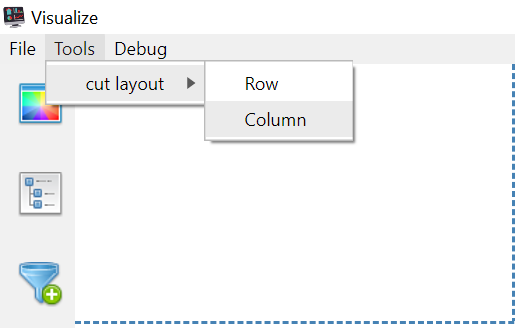
\includegraphics[width=.8\linewidth]{figures/divisor1.png}  
  \caption{seleção de modo de criação de divisões}
  \label{fig:sub-first}
\end{subfigure}
\begin{subfigure}{.5\textwidth}
  \centering
  % include second image
  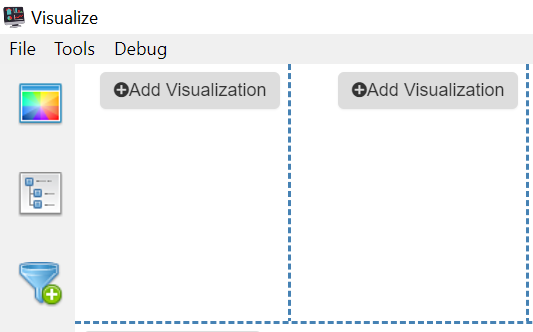
\includegraphics[width=.8\linewidth]{figures/divisor2.png}  
  \caption{criação de divisão horizontal após selecionar o método de divisão}
  \label{fig:sub-second}
\end{subfigure}
\caption{Ferramenta para criação de divisões para novas visualizações orientado por linhas e colunas}
\label{fig_layout}
\end{figure}



Cada espaço do layout pode ser incluída uma visualização e as visualizações podem ser customizadas com dados, além disso, após criado um layout de posições de tela o mesmo pode ser salvo, redimensionado, exportado e importado em um arquivo formato JSON pela ferramenta para utilizações posteriores e novas customizações, esse fluxo é apresentado na \autoref{fig_fluxo}.

\begin{figure}[h]
	\caption{\label{fig_fluxo} Fluxo de criação de \textit{dashboard} na aplicação desenvolvida}
	\begin{center}
	    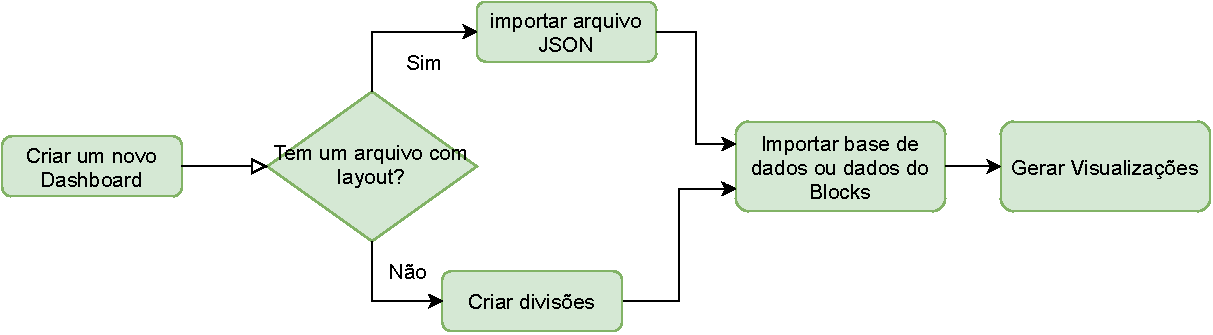
\includegraphics[width=\textwidth,scale=1]{figures/Diagrama de fluxo tcc.pdf}
	\end{center}
	\legend{Fonte: O autor}
\end{figure}

\section{Arquitetura}
A Arquitetura organizacional do projeto foi definida como um MVC (\textit{Model, View, Controller}) definido por \cite{deacon2009model}, como um modelo com três camadas: modelo, responsável pela estrutura de dados, visão, a interface gráfica disponibilizada para o usuário, e o controlador, responsável por conter a regra de negócio da aplicação. A arquitetura foi desenvolvida em um modelo incremental com constantes reuniões para discussão para propostas de melhorias e novas funcionalidades na ferramenta. 

No desenvolvimento foi selecionada a linguagem de programação \textit{javacript} ou \textit{Ecmascript 6} aproveitando de seus novos recursos como \textit{Arrow Functions}, \textit{Array Destructuring} e classes, em conjunto com o \textit{framework} \textit{Electron} \cite{electron} para criação de uma aplicação \textit{desktop} compatível com sistemas operacionais Windows, Linux e Mac, além disso, os gráficos disponíveis foram implementados no Vistechlib uma biblioteca de módulos reutilizáveis de visualização da informação \cite{Vistechlib}. Bem como, foi implementado um modulo de leitura das bases de dados para converter objetos CSV, JSON, TSV e tratar os dados categóricos e contínuos, e adicioná-los na ferramenta para filtros e seleções. Também foi criada uma estrutura de comunicação por \textit{sockets} para comunicar a aplicação desenvolvida com a ferramenta de geração de dados \textit{Blocks} \cite{blocks} que requisita esses dados para gerar visualizações.


A \autoref{mvc_app} contém uma representação do fluxo de troca de informações na ferramenta e sua estrutura MVC mencionada anteriormente e suas principais atividades de cada camada. No \textsf{model} como mostrado na \autoref{mvc_app} contém dois principais módulos, o de ''leitura de dados e conversão'' onde é feita a leitura da base de dados e sumarizado para ferramenta para serem interpretados pelas visualizações e interfaces, bem como o módulo de estrutura de \textsf{layout} onde pode ser carregado um arquivo JSON que contém as posições, divisões, tamanhos das estruturas de tela e visualizações que podem ser importadas e exportadas para utilizações posteriores.

\begin{figure}[h]
    
	\caption{Arquitetura MVC da ferramenta desenvolvida, seus principais componentes, trocas de informações disponíveis nos módulos do sistema. A camada \textit{model} onde contém as estruturas de dados, o \textit{controller} com as regras de criações de visualizações e criação de  \textit{layout} de tela, e a  \textit{view} com as interfaces para o usuário}
	\label{mvc_app}
	\begin{center}
	    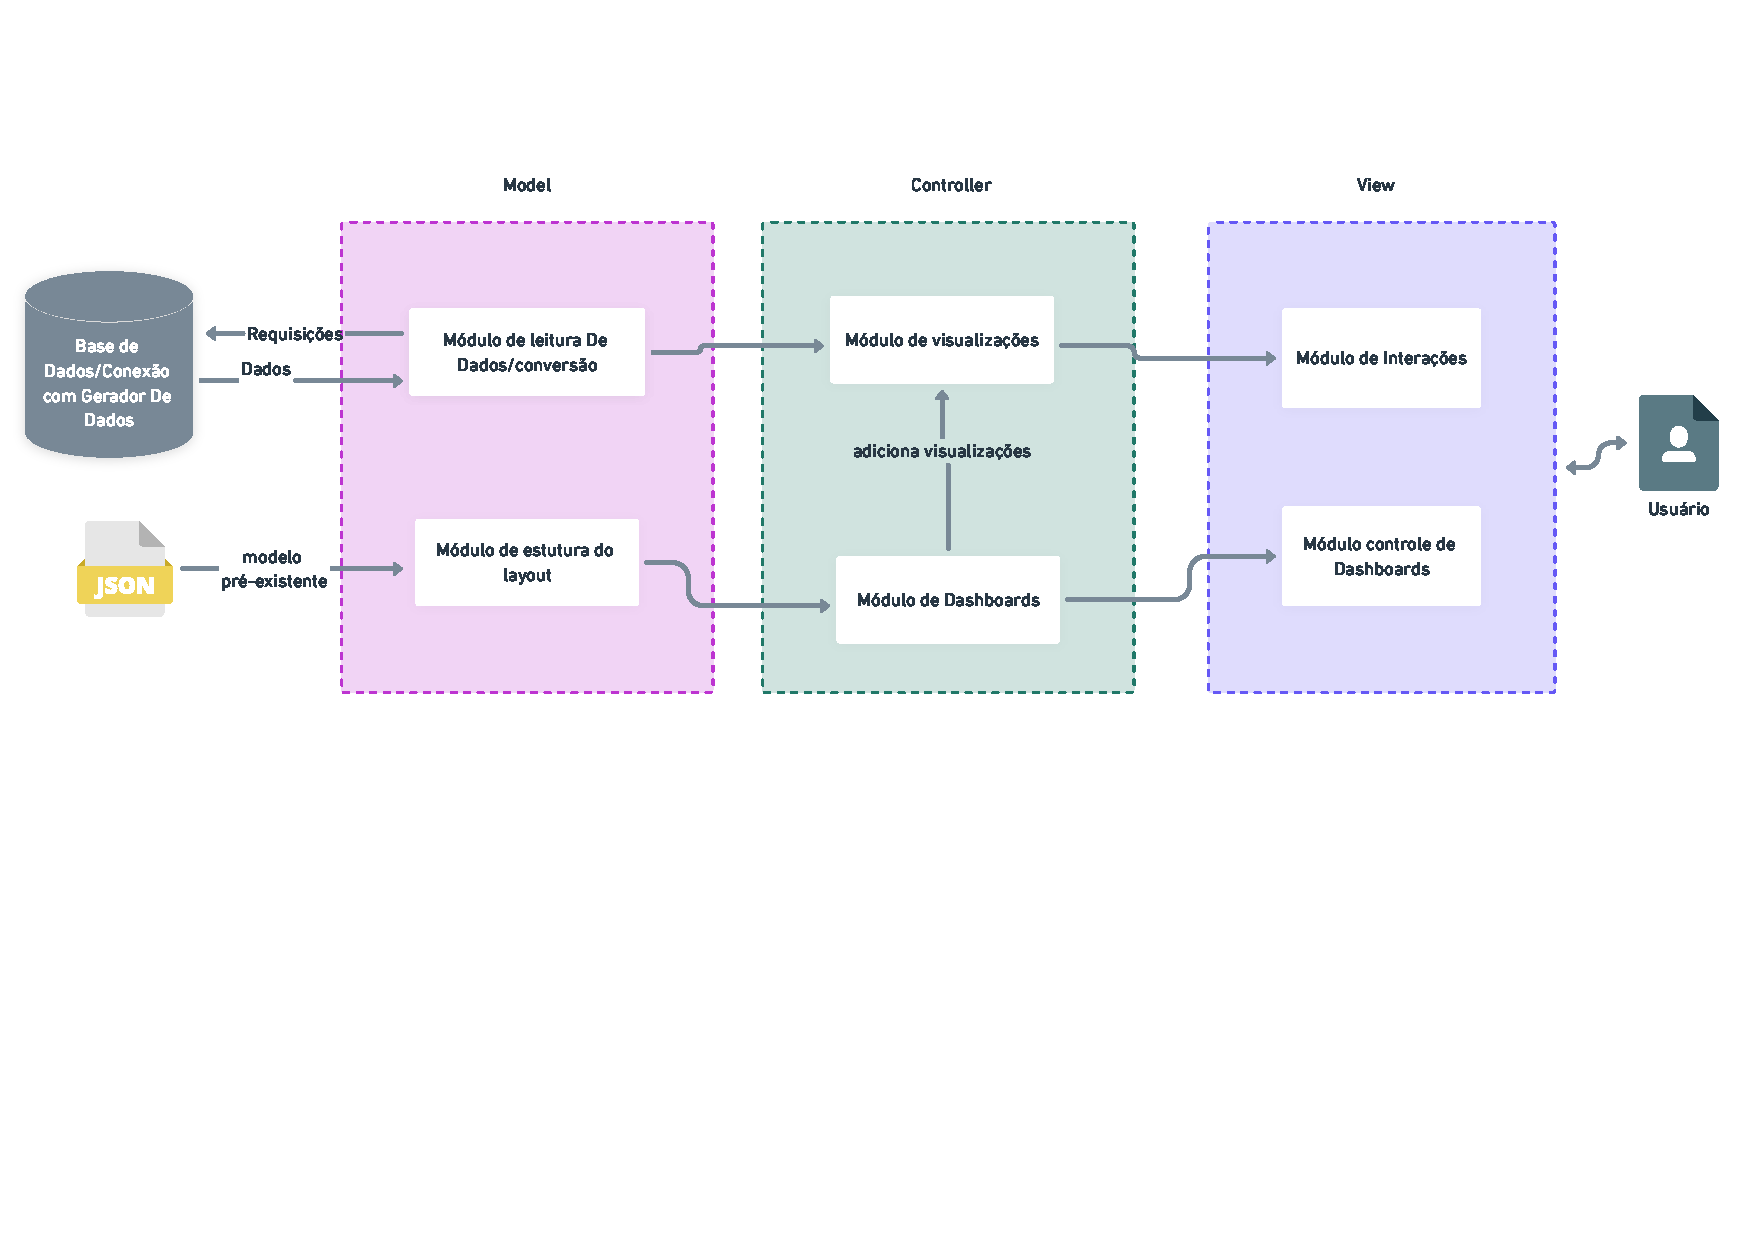
\includegraphics[width=30pc,trim={0 260 0 0}]{figures/mvc_diagrama.pdf}
	\end{center}
	\legend{Fonte: O autor}
\end{figure}


Já no \textit{controller} podemos ver os seguintes módulos que contém a regra de negócio se comunicando com os \textit{models} e \textit{view} que são respectivamente o módulo de visualizações responsável por criar, customizar, deletar e oferecer as interações das visualizações e o módulo de \textit{dashboards} que tem como finalidade a criação e customização das subdivisões para criação dos \textit{dashboards}.

Na \textit{view} contém o módulo de interações e o módulo controle de \textit{dashboards}, que são as interfaces gráficas onde o usuário realiza por meio do mouse suas interações para customizar gráficos e subdivisões de telas.



\section{Diagrama de casos de uso}
Nesta seção serão abordados os casos de uso da aplicação, os fluxos e as principais utilizações pelo usuário da ferramenta.

As possibilidades de uso da ferramenta pelo usuário estão descritas no diagrama de casos de uso na \autoref{casos_de_uso_uml}, onde nessa figura estão descritas as funcionalidades disponíveis da ferramenta.

O diagrama de casos de uso na \autoref{casos_de_uso_uml} ilustra os possíveis fluxos de criação de \textit{dashboard}, desde a criação do layout até a interação nas visualizações disponíveis ou, caso seja desejo do usuário, a criação de apenas uma visualização e exploração por meio de interações, bem como o carregamento de um \textit{dashboard} pré-existente gerado pela ferramenta também pode ser realizado.

\begin{figure}
	\caption{\label{casos_de_uso_uml}Diagrama de casos de uso da ferramenta para criação de um novo \textit{dashboard} ou visualização }
	\begin{center}
	    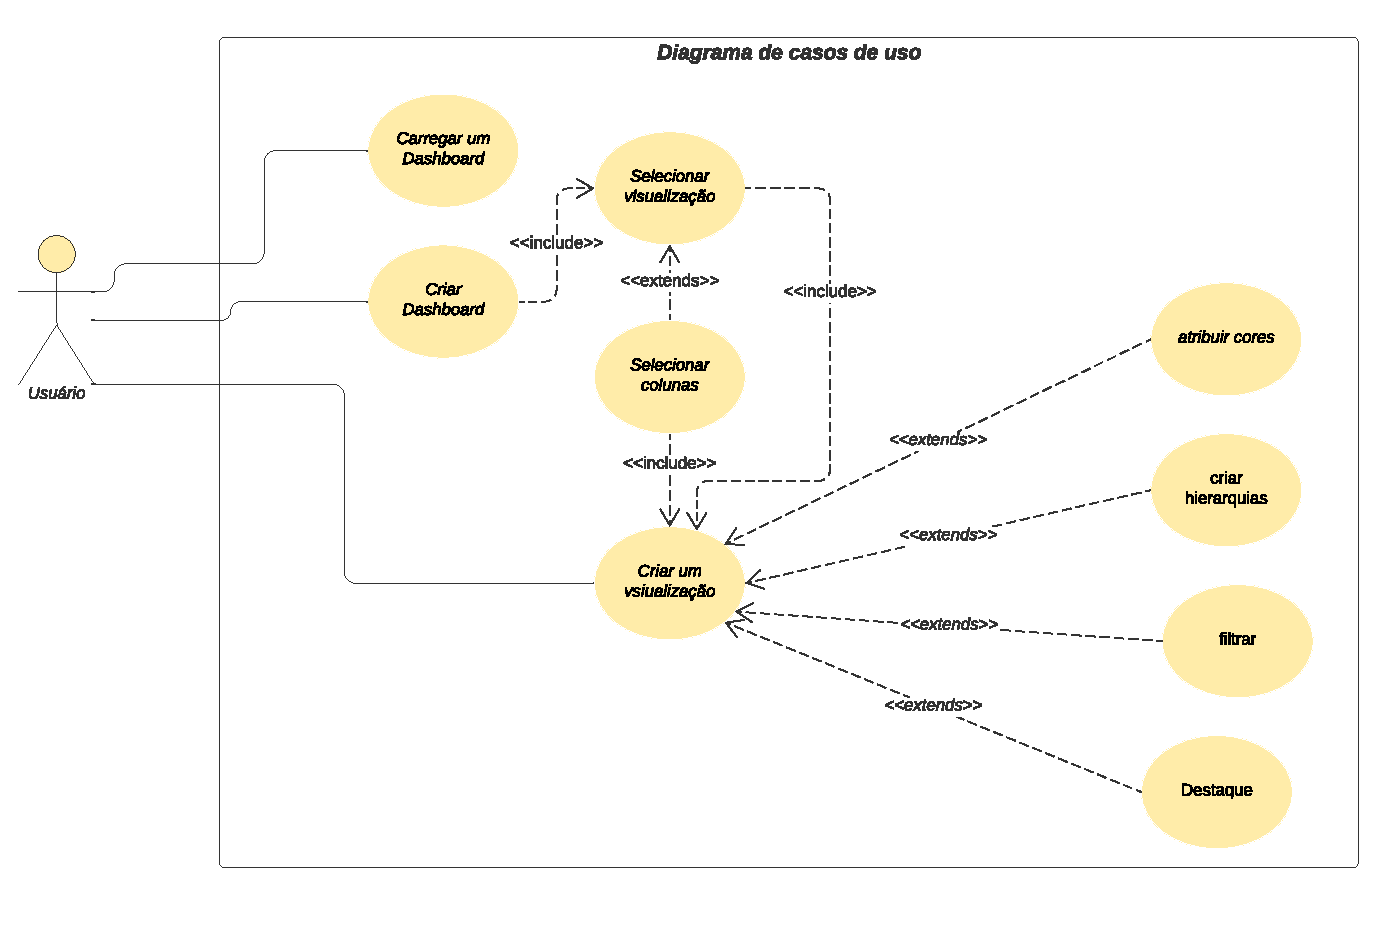
\includegraphics[width=35pc]{figures/Diagrama de casos de uso.pdf}
	\end{center}
	\legend{Fonte: O autor}
\end{figure}

\section{Diagrama de classes}
O diagrama de classes demonstrado na \autoref{classe_uml} exemplifica a estrutura de classes resumida para a geração dos gráficos. A classe abstrata \textit{Visualization}  possui os métodos e atributos onde cada subclasse de gráfico irá sobrescrever e herdar os comportamentos da classe abstrata. Os principais métodos disponíveis na classe abstrata compartilhada com as subclasses são  \textit{data()},  \textit{redraw()},  \textit{resize()}, e \textit{bindMouseEvents()}. Esses métodos respectivamente são responsáveis por \textit{data()} processar e atribuir os dados para um objeto, \textit{redraw()} é o método onde contém a lógica de desenho para cada gráfico utilizando d3.js, o método \textit{resize()} tem a responsabilidade de redimensionar o tamanho do gráfico conforme o tamanho disponível em tela ou subdivisão de tela, já o método \textit{bindMouseEvents()} visa permitir a interação com o mouse nos componentes equivalentes aos dados.

A segunda parte da \autoref{classe_uml} demonstra o controlador de interações para cada visualização seguindo o padrão clássico \textit{Strategy} catalogado no trabalho de \cite{gamma1995design}. A classe \textit{Interaction Mananger} tem o objetivo de fornecer os métodos para que as interações possam ser selecionadas \textit{select()}, desselecionadas \textit{unselected()}, e desativadas \textit{disable()}, a importância desse método é permitir que, em tempo de execução, as interações sejam trocadas rapidamente e não gerem conflitos para o usuário final.

O Diagrama na \autoref{classe_uml_layout}  representa as classes responsáveis pela geração do layout customizável para criação de novas divisões, onde serão organizados as visualizações, criando um \textit{dashboard} ao final, essa geração pode ser feita em tempo real com cliques no \textit{mouse} ou realizada com base em um arquivo JSON. No diagrama de classe da \autoref{classe_uml_layout} podemos ver a relação de composição do layout dinâmico de \textit{dashboards} onde temos as classes \textit{PartitionLayout} que contém os elementos redimensionáveis e que podem ser divididos, a classe \textit{Partition} onde é criada uma partição horizontal ou vertical, criando uma nova divisão no HTML, e a classe \textit{Divisor} que representa a linha divisória e redimensionável do layout com uma composição da classe \textit{PlaceHolderDivisor} para verificar cálculos e mostrar a interação de redimensionamento das divisões na tela.


\begin{figure}
	\caption{\label{classe_uml}Diagrama de classes para a geração das visualizações e seus métodos em conjunto com as classes para controlar as interações.}
	\begin{center}
	    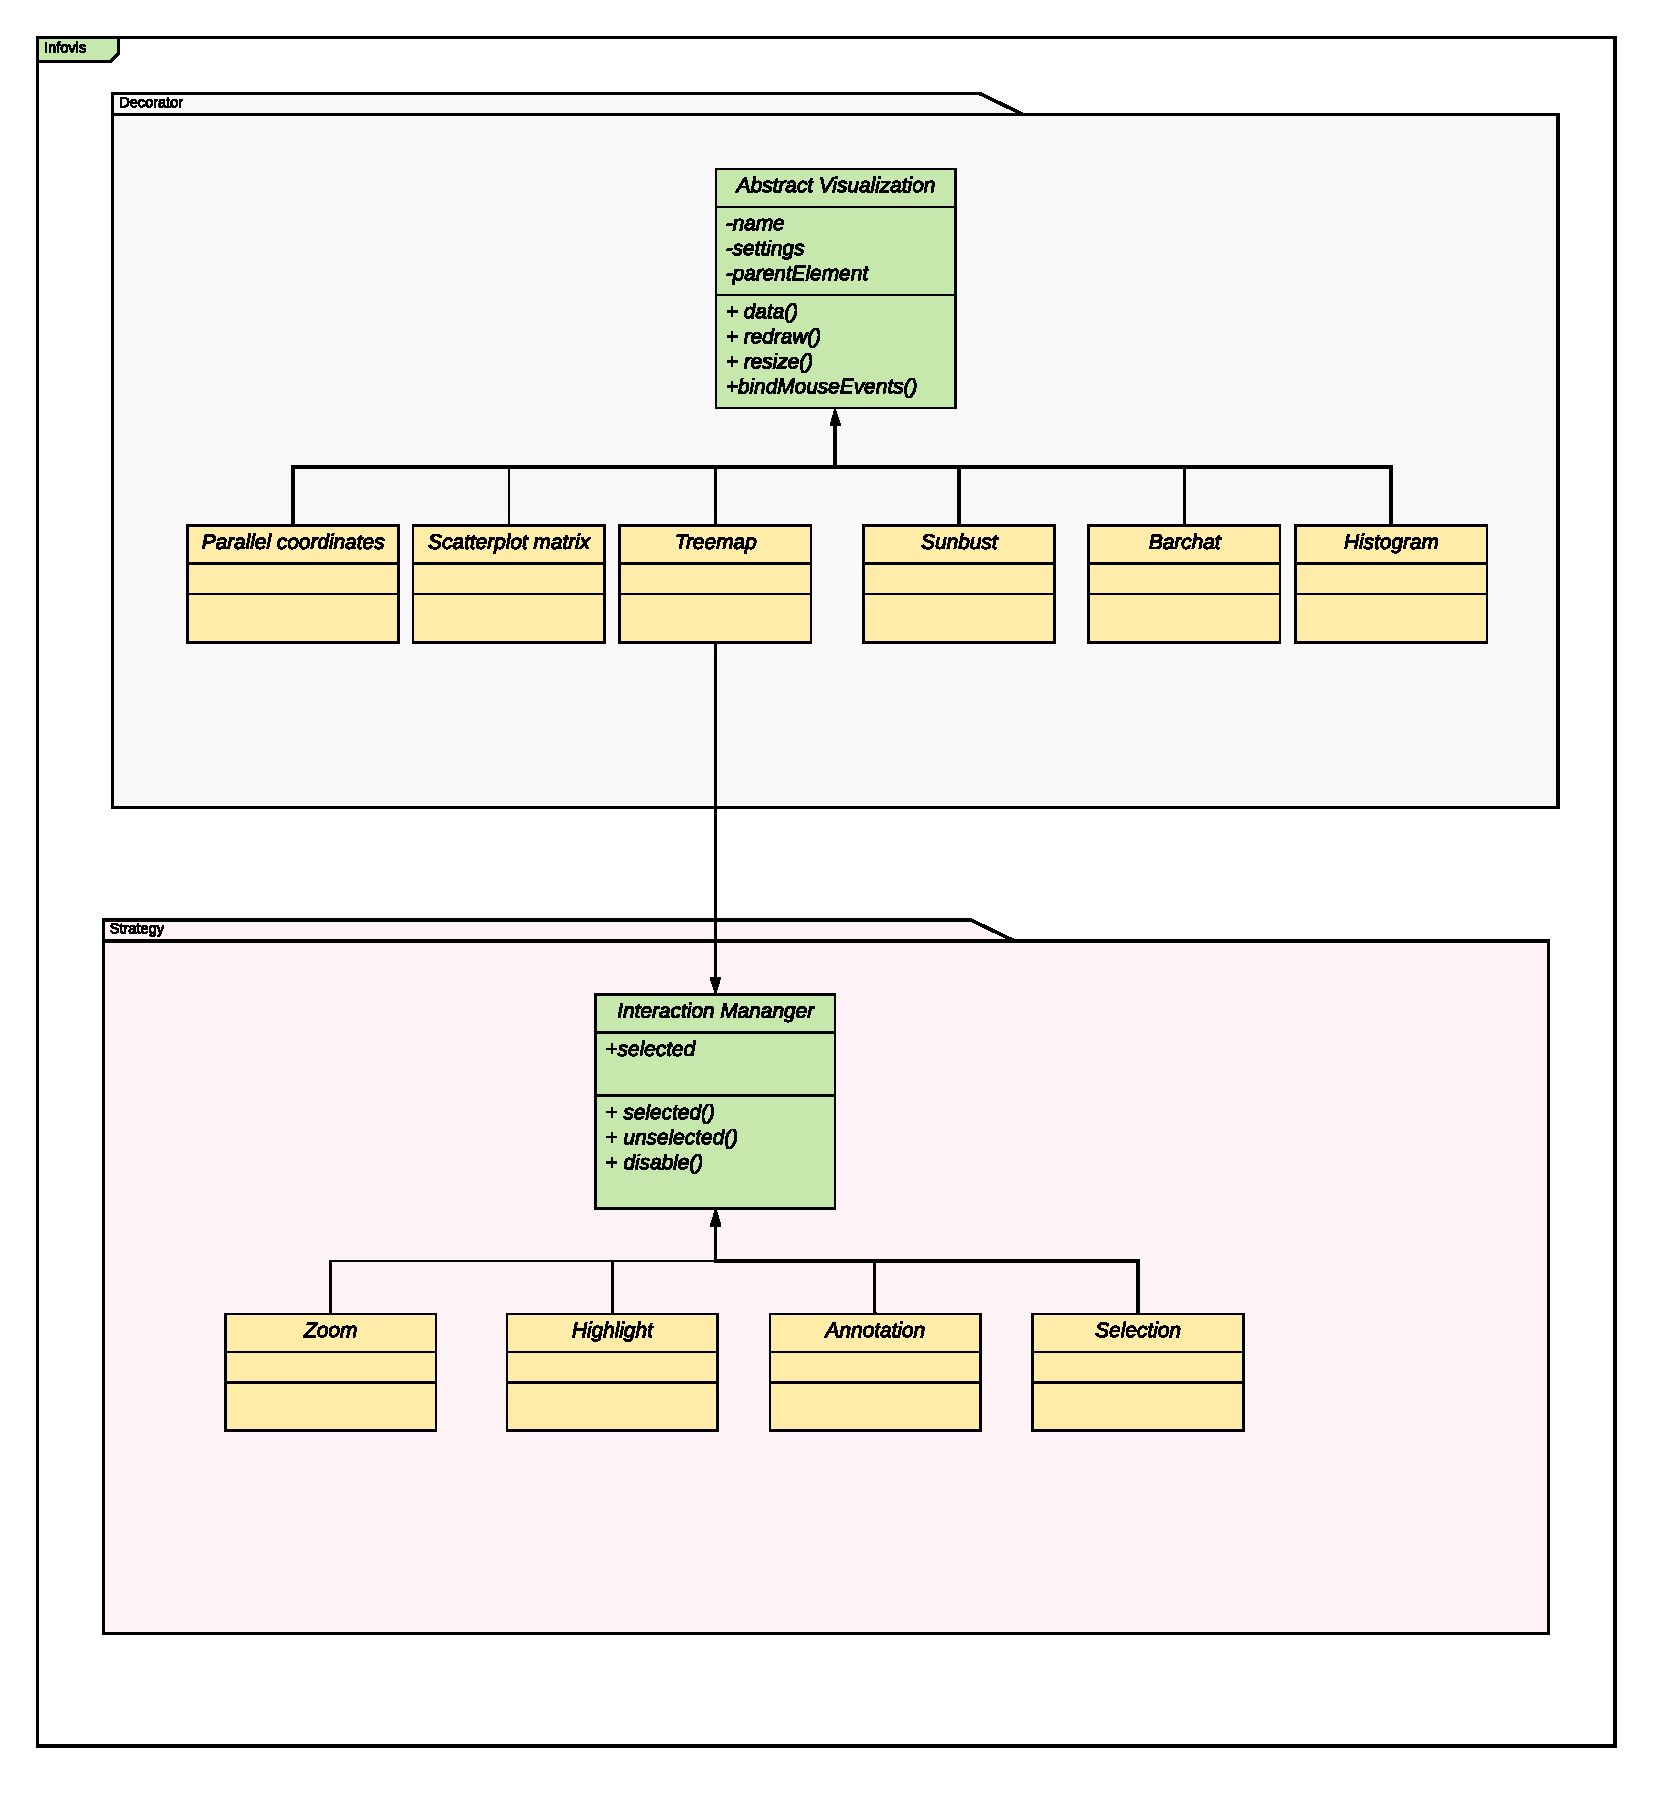
\includegraphics[width=35pc,height=35pc]{figures/visApplication uml(1).pdf}
	\end{center}
	\legend{Fonte: O autor}
\end{figure}

\begin{figure}
	\caption{\label{classe_uml_layout}Diagrama de classes para a geração dos layout interativos para criação dos \textit{dashboards} onde as classes \textit{PartitionLayout}, \textit{Partion}, \textit{Divisor}, \textit{PlaceHolderDivisor}, tem uma relação de composição na qual são dependentes para existirem.}
	\begin{center}
	    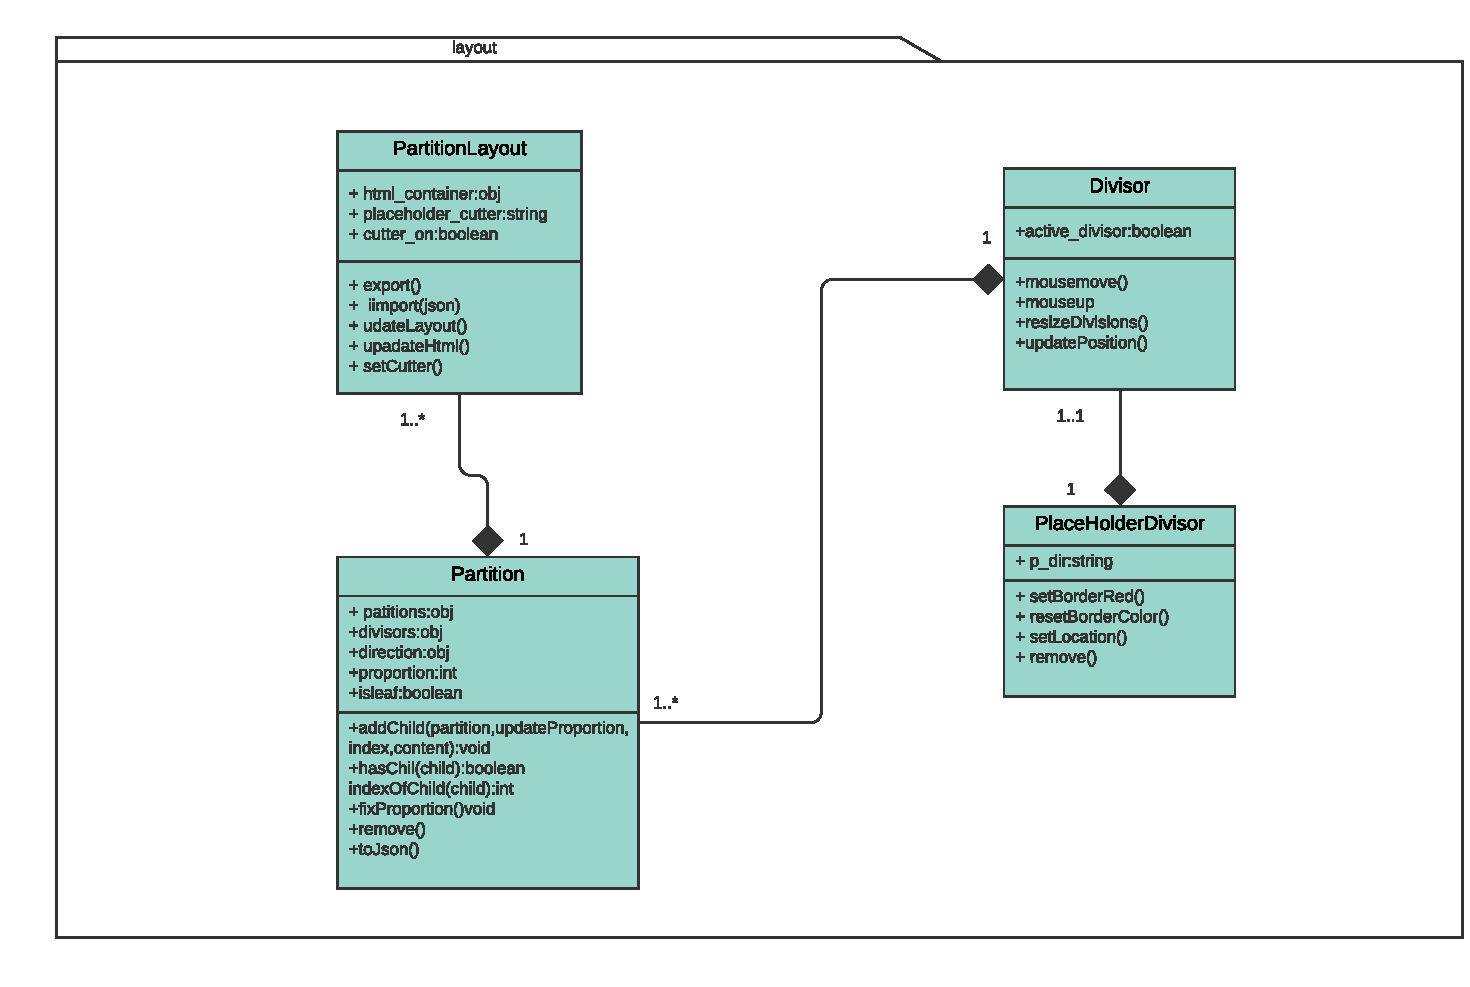
\includegraphics[width=\textwidth,height=30pc]{figures/Diagrama layout parrtition.pdf}
	\end{center}
	\legend{Fonte: O autor}
\end{figure}




\section{Protótipo}
O Protótipo é responsável pela construção das visualizações de dados, assim como pela criação dos layouts de  \textit{dashboards}, sendo assim, é possível utilizar visualizações únicas seguindo o \textit{pipeline} clássico de visualização de dados, transformando os dados em dados tabulares e convertendo as estruturas em variáveis visuais que compõem uma visualização completa com interações fornecidas ao usuário final.  

Nas funcionalidades do protótipo, um dos principais destaques é a criação de \textit{dashboards} dinâmicos provenientes de divisões horizontais e verticais onde, a tela pode ser subdividida em uma dessas divisões, pode ser selecionada qual visualização ficará nesse local dependendo da vontade do usuário.
As interações ocorrem por meio do mouse, onde é possível subdividir a tela, a partir das posições do mouse, bem como, também é possível carregar um arquivo JSON com o formato gerado pela ferramenta com um layout de tela já pré-existente.  

\subsection{Visualizações Disponíveis}
Nesta seção serão apresentas as visualizações disponíveis no protótipo desenvolvido, diversas visualizações foram implementadas com diferentes objetivos, como visualizações multidimensionais, unidimensionais, hierárquicas, árvores, e visualizações de linha. As visualizações disponíveis são \textit{Beeswarm Plot}, textit{Circle Packing}, \textit{Coordenadas Paralelas}, Gráfico de Barras,\textit{Histograma}, Matriz de \textit{Scatter Plot},coordenadas paralelas, \textit{Sunburst} e \textit{Treemap}, abordadas abaixo: 

\textbf{\textit{Beeswarm Plot}}:
    Pode ser descrito como um gráfico de dispersão unidimensional semelhante a um enxame de abelhas onde os pontos não se sobrepõem e cada item representa uma posição em relação ao eixo de valor, além do posicionamento, os pontos podem conter um valor atribuído a uma cor, como exemplo \autoref{fig_dash_bars}.
    
\textbf{Gráfico de Barras}:
    O gráfico de barras verticais pode ser descrito como um conjunto de barras retangulares onde o comprimento é proporcional aos valores que estão sendo representados. Os eixos demonstram o que está sendo comparado nas barras, sendo que a ilustração de um gráfico de barras gerado pela aplicação pode ser visualizada na \autoref{fig_dash_bars}
    
\textbf{Histograma}:
    O gráfico de histograma é composto por barras sequenciais em sua versão implementada na ferramenta disponível na \autoref{fig_dash_bars} onde representam a distribuição de frequência, no histograma cada barra representa um registro ou dado, bem como a altura representa o valor desse registro utilizado para dados contínuos, o histograma tem como objetivo observar a distribuição da amostragem selecionada.
    
\begin{figure}[h]
	\caption{\label{fig_dash_bars} Exemplo de gráficos implementados e disponíveis na aplicação \textit{Beeswarm plot}, Gráfico de Barras, e Histograma.}
	\begin{center}
	    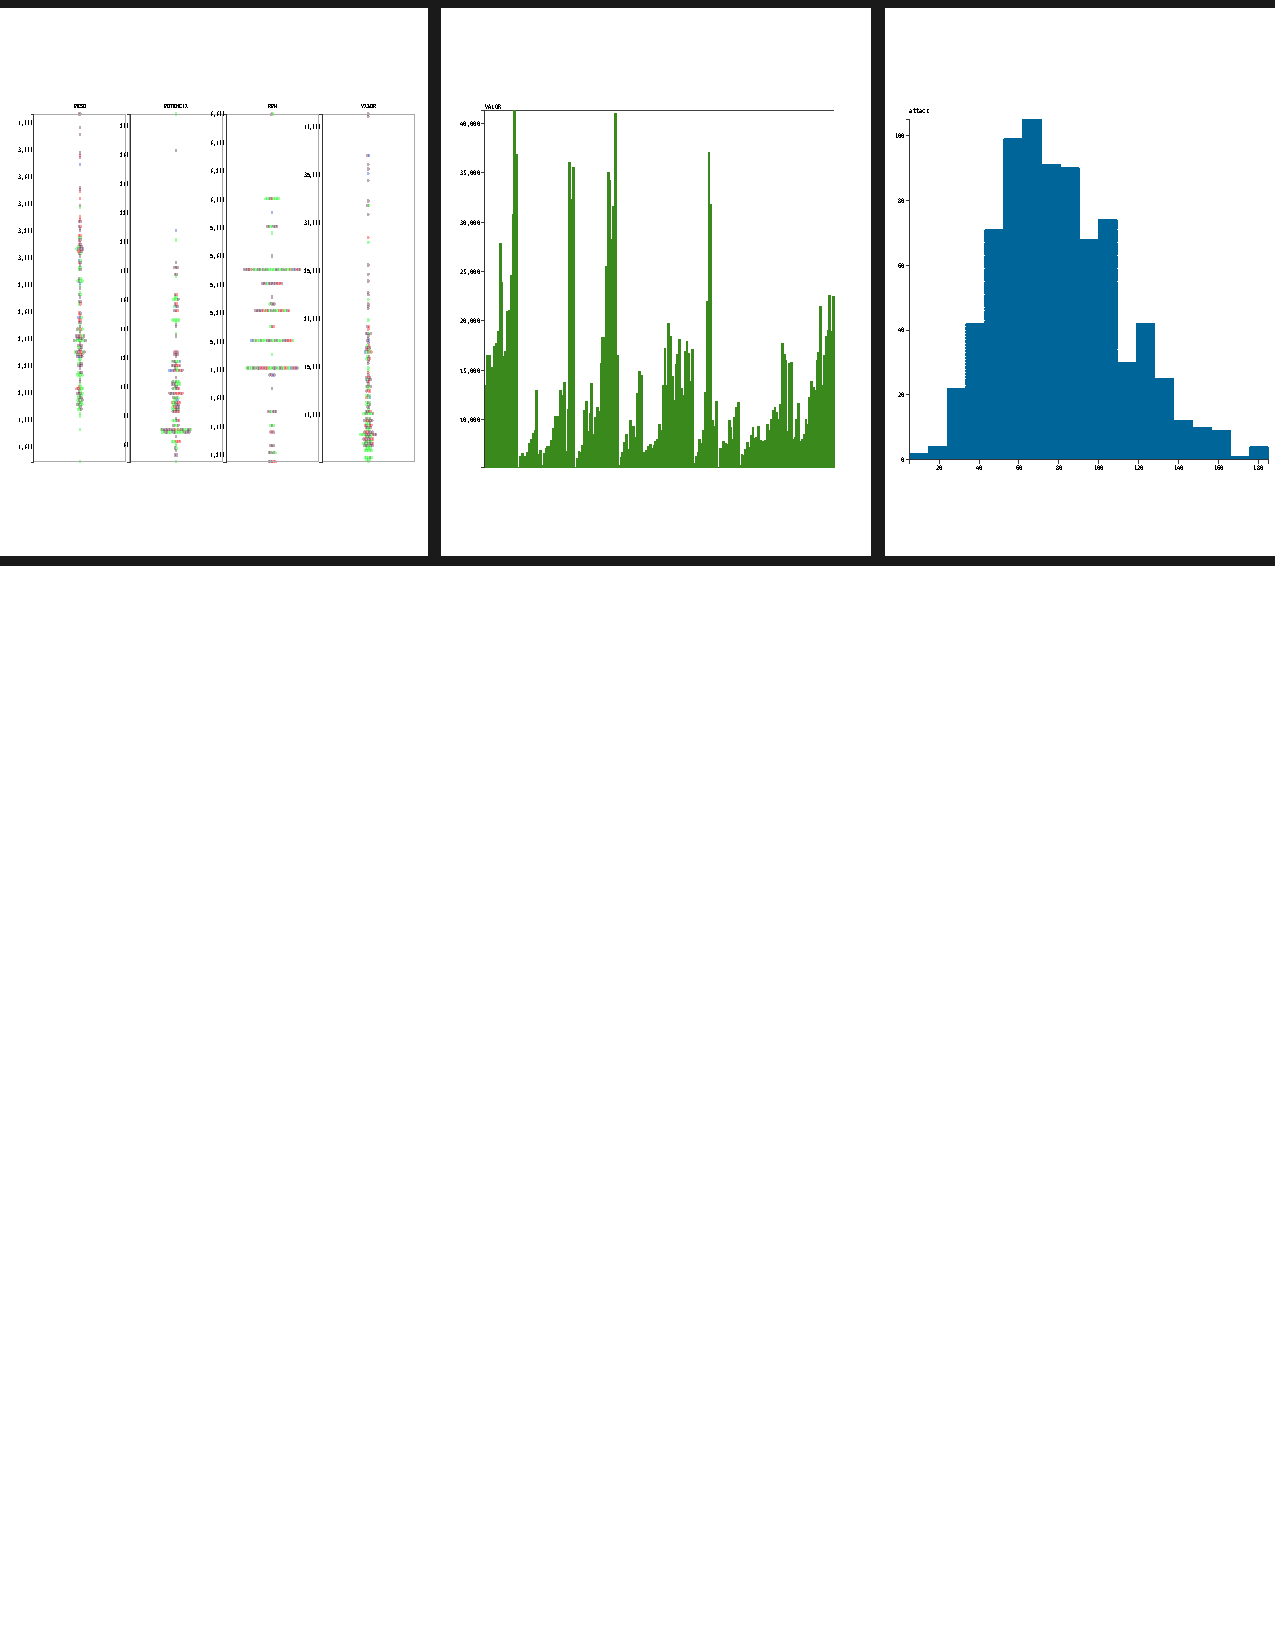
\includegraphics[width=\textwidth,size=1, trim={0mm 180mm, 0mm 0mm},clip]{figures/garficos_2.pdf}
	\end{center}
	\legend{Fonte: O autor}
\end{figure}

\textbf{\textit{Treemap}}: A técnica  \textit{Treemap} foi desenvolvida por \cite{johnson1999tree} e visa representar dados hierárquicos com uma proposta de preenchimento de espaços com itens retangulares. Nessa variação da técnica \textit{treemap} selecionada foi o \textit{treemap squarified} a qual os itens tentam manter uma estrutura aproximadamente quadrada, onde as visualizações se adaptam ao espaço disponível e ocupam completamente o espaço. O \textit{treemap} pode conter organizações de hierarquias, serem atribuídas as cores, rótulos nos registros retangulares folhas ilustradas na \autoref{graficos_hie}. 

\textbf{\textit{Circle Packing}}:
    Pode ser descrito como uma técnica de visualização de empacotamento de círculos na qual, pode ou não existir hierarquia. Aos itens podem ser atribuídas cores, enquanto os tamanhos podem codificar uma variável da base de dados, por exemplo, na \autoref{graficos_hie} onde são ilustradas as hierarquias, cores e tamanhos representando valores da base de dados.
    
\textbf{\textit{Sunburst}}:
    A técnica \textit{Sunburst} é uma visualização de dados em formato radial hierárquica, descrito por \cite{Stasko}  como uma árvore radial, ilustrada na \autoref{graficos_hie}, onde cada anel simboliza um nível de hierarquia tendo como centro o nó raiz, e os demais itens dos anéis podem ser divididos conforme os valores daquele nível, nas extremidades podemos ver nos respectivos nós folhas os dados de cada item como uma fatia.
    
    
\begin{figure}[h]
	\caption{\label{graficos_hie} Exemplo de gráficos implementados e disponíveis na aplicação \textit{Treemap},  \textit{Circle Packing}, e  \textit{Sunburst}. }
	\begin{center}
	    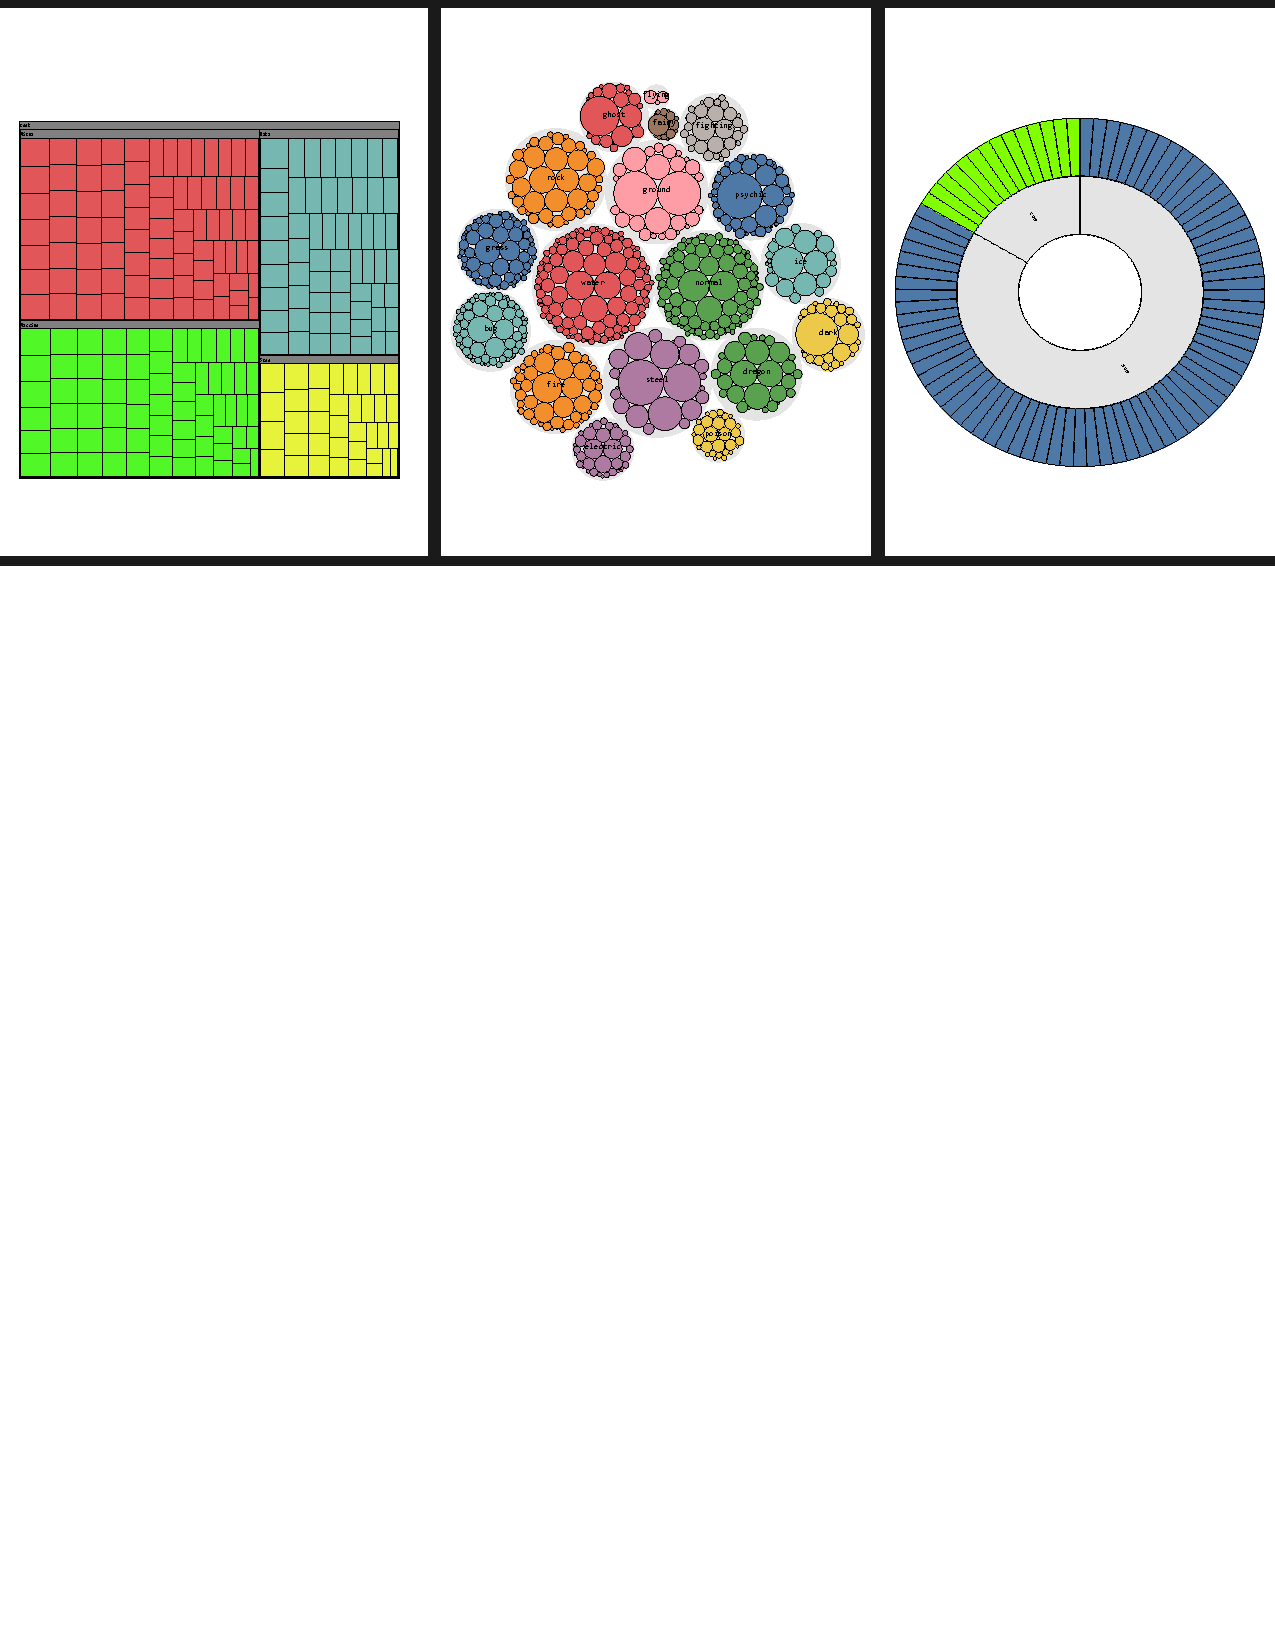
\includegraphics[width=\textwidth,size=1, trim={0mm 180mm, 0mm 0mm},clip]{figures/garficos_1.pdf}
	\end{center}
	\legend{Fonte: O autor}
\end{figure}

\textbf{Matriz de \textit{Scatter Plot}}:
    É uma técnica 2D onde reúne uma grade de gráficos de dispersão com valores que podem ser codificados para eixo X, eixo Y, cor e forma, sendo demonstrado sua implementação na ferramenta na \autoref{graf_3}.
    
\textbf{Coordenadas Paralelas}:
    A técnica de coordenadas paralelas ilustrada na \autoref{graf_3}, desenvolvida por \cite{inselberg1985plane} apresenta uma visualização para dados multidimensionais, onde eixos paralelos verticais ou horizontais são exibidos na tela para representar as dimensões e linha ou polígonos que atravessam esses eixos em uma posição delimitando os valores dos registros nessa dimensão. Eixos podem ser reordenados e as cores também podem representar uma dimensão.

\textbf{\textit{Parallel Bundling}}: É uma técnica de visualização baseada na técnica de coordenadas paralelas elaborada por \cite{divino2017visual} com as características de eixos e linhas semelhantes às coordenadas paralelas em união com a técnica \cite{zhou2013edge} de agrupamento de arestas, agrupando informações em um eixo onde pode conter características das informações do agrupamento dependendo da curva disposta para cada agrupamento ilustrado na \autoref{graf_3}.
    
    
 \begin{figure}[h]
	\caption{\label{graf_3} Exemplo de gráficos implementados e disponíveis na aplicação respectivamente Matriz de \textit{Scatter Plot}, Coordenadas Paralelas, e \textit{Parallel Bundling}}
	\begin{center}
	    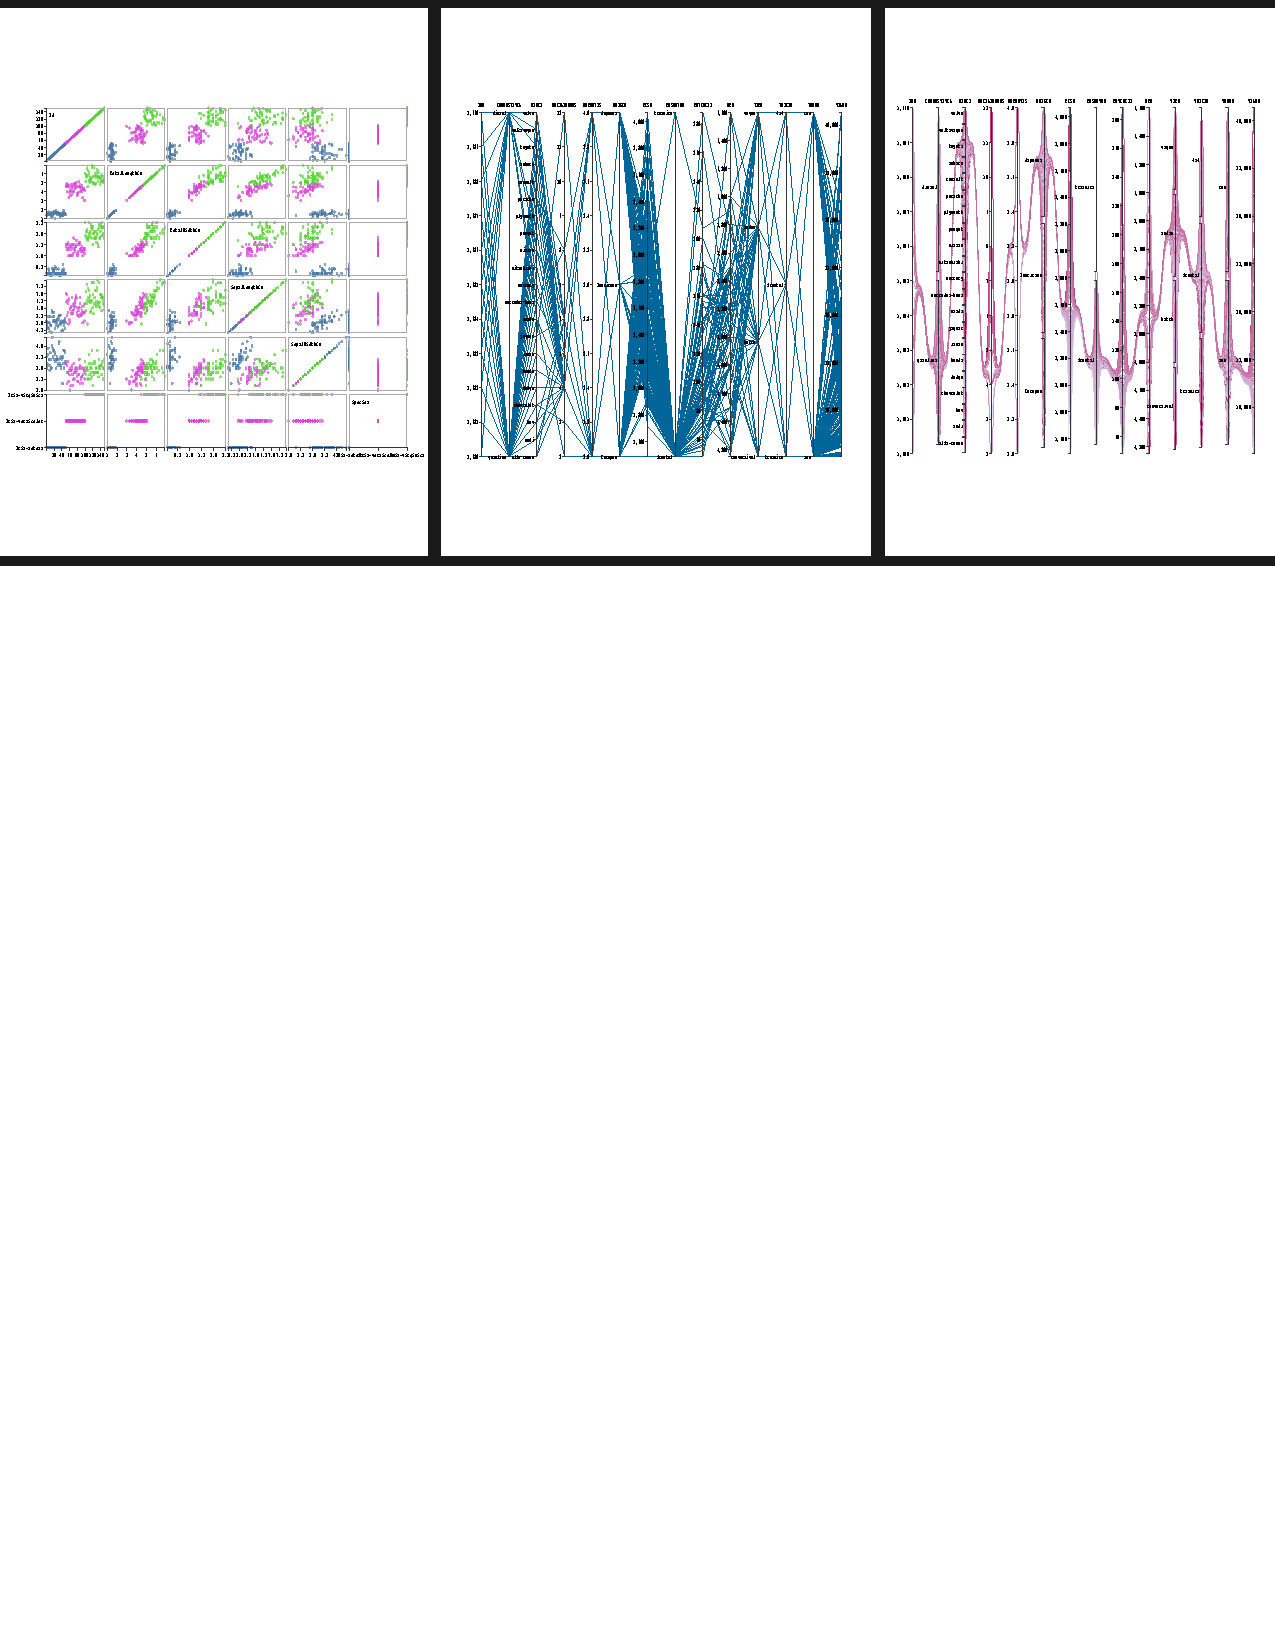
\includegraphics[width=\textwidth,size=1, trim={0mm 180mm, 0mm 0mm},clip]{figures/garficos_3.pdf}
	\end{center}
	\legend{Fonte: O autor}
\end{figure}
    


\section{Funcionalidades}

O ambiente de criação das visualizações da ferramenta é um layout de partições redimensionáveis, demonstrado na \autoref{layout_resize}, onde ficarão as visualizações, sendo possível configurar livremente o tamanho das visualizações, quais serão redimensionadas conforme o tamanho disponível, além disso, é possível utilizar as visualizações em ambientes de múltiplas telas e \textit{large display}, desse modo é  possível coordenar diferentes visualizações simultaneamente como ilustrado na \autoref{visualizations}.

\begin{figure}[!htb]
	\caption{\label{visualizations} Telas da aplicação com todas as visualizações disponíveis
}
	\begin{center}
	    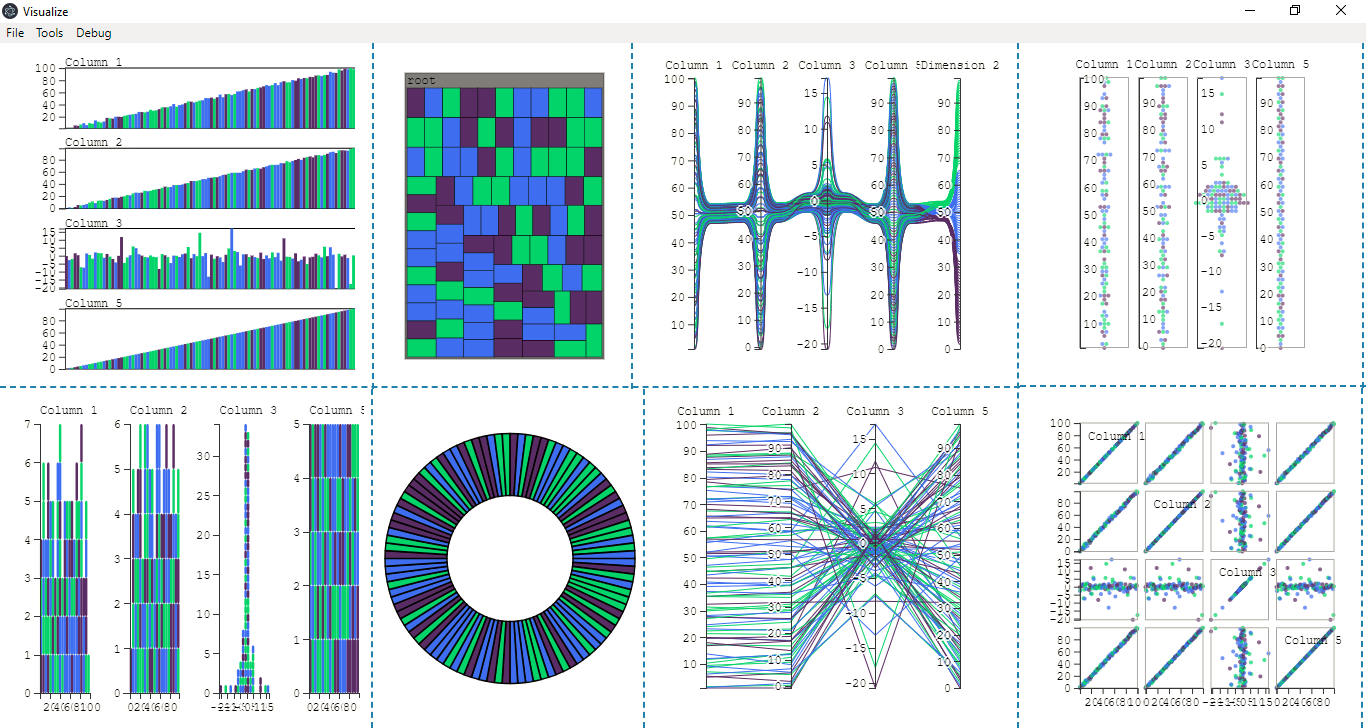
\includegraphics[width=\textwidth,size=1]{figures/Capturar1.PNG}
	\end{center}
	\legend{Fonte: O autor}
\end{figure}


\begin{figure}[!htb]
	\caption{\label{layout_resize} Telas de layout dinâmicos, as áreas destacadas representam: (1)- pontos representação redimensionar a tela, (2)- botão de criação das visualizações,(3) – criação de uma nova partição para visualizações.
}
	\begin{center}
	    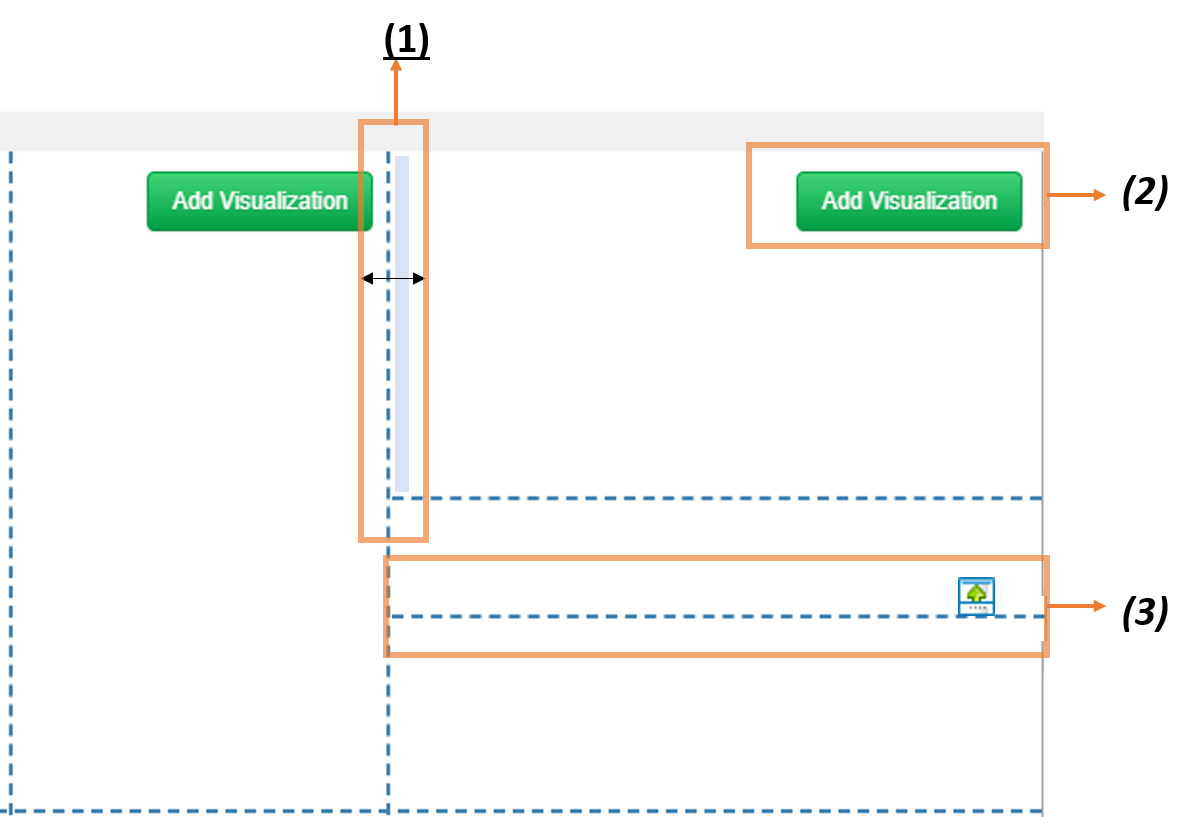
\includegraphics[width=30pc,scale=1]{figures/layouts.png}
	\end{center}
	\legend{Fonte: O autor}
\end{figure}

\section{Interações}
Segundo \cite{ward2010interactive} interações, no contexto de visualização de dados, são mecanismos disponíveis para modificar o que é visível pelo usuário. Existem diversas técnicas de interação como seleção, filtro, navegação, zoom, reconfigurar os dados e hierarquias, conectar dados em diferentes visualizações e objetos, e destaque. 

A ferramenta oferece interações e configurações, assim os usuários, seguindo os princípios de exploração visual:  \textit{“overview, first zoom and filter, then details-on-demand”} e seguindo os princípios principais de uma ferramenta de \textit{INFOVIS} definidos por \cite{Shneiderman1996},
Esses princípios têm como objetivo proporcionar aos usuários o \textit{overview} uma visão geral dos dados e problema apresentado, como primeiras interações um zoom proporcionando a entrada em detalhes e o filtro permitindo tirar informações dependendo da problemática e por último os detalhes sobre demanda permitindo observar particularidades de uma determinado item. A aplicação proporciona uma fácil manipulação e configuração das visualizações, com alta flexibilidade, permitindo filtros e seleções, sendo possível criar seleções, filtros, seleção de cor por atributo, hierarquias nas diversas visualizações. Sendo possível definir por meio das configurações de interfaces pelo usuário as interações e suas funcionalidades por meio dos ícones exemplificados na \autoref{img_icones}, no qual explica cada ícone de interação e suas respectivas funcionalidades.


\begin{figure}[ht]
	\caption{\label{img_icones} Explicação do significado dos ícones de interação para as visualizações disponíveis.
}
	\begin{center}
	    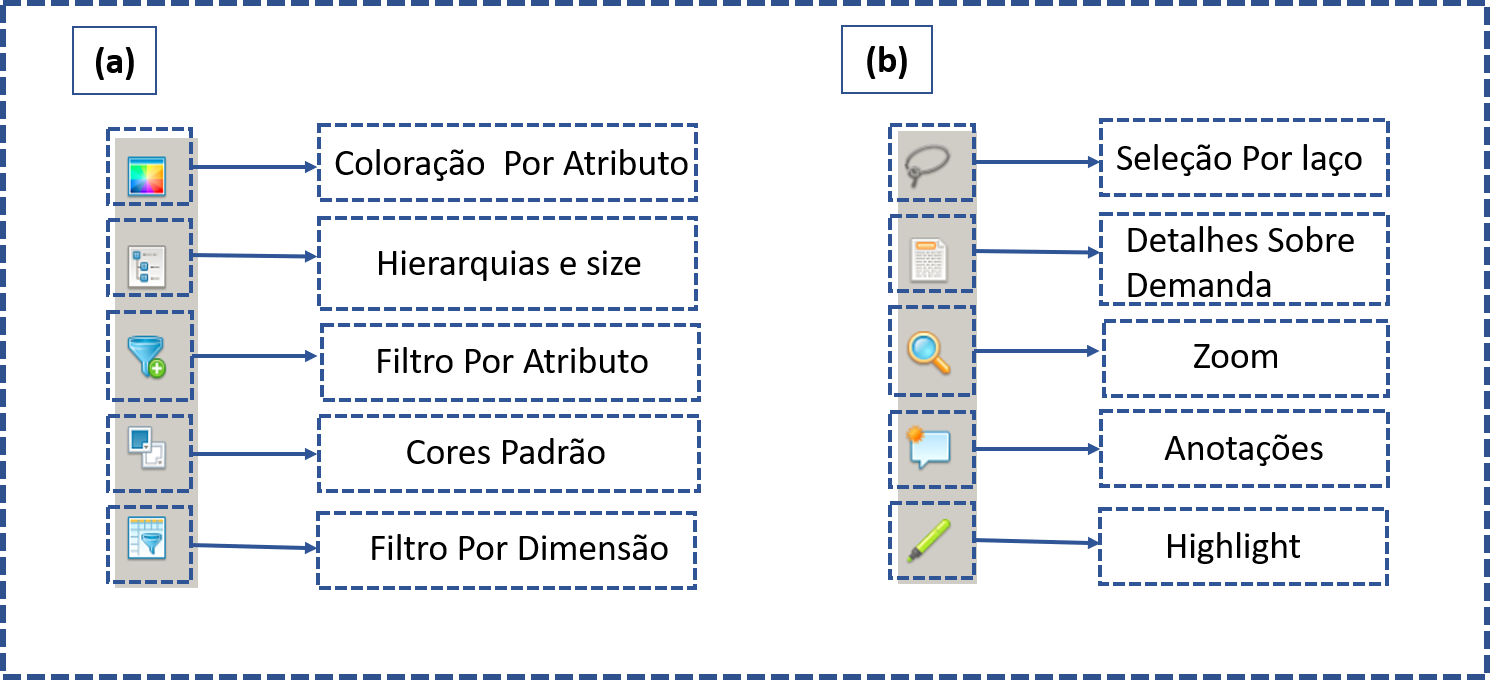
\includegraphics[width=30pc]{figures/img_icones.png}
	\end{center}
	\legend{Fonte: O autor}
\end{figure}

     

\subsection{Coloração por atributo}
Nessa funcionalidade é possível selecionar atributos categóricos e contínuos, caso os atributos sejam categóricos a ferramenta permite a personalização de cor para cada atributo, caso sejam contínuos é possível escolher as cores do intervalo entre o valor mínimo e máximo. Bem como, cada visualização também vai seguir o padrão de cores selecionado para cada atributo.


\begin{figure}[!ht]
	\caption{\label{fig_color_visualization} Exemplo de visualizações com coloração por um atributo contínuo e menu de interações para seleção de cores para atributos categóricos e contínuos.
}
	\begin{center}
	    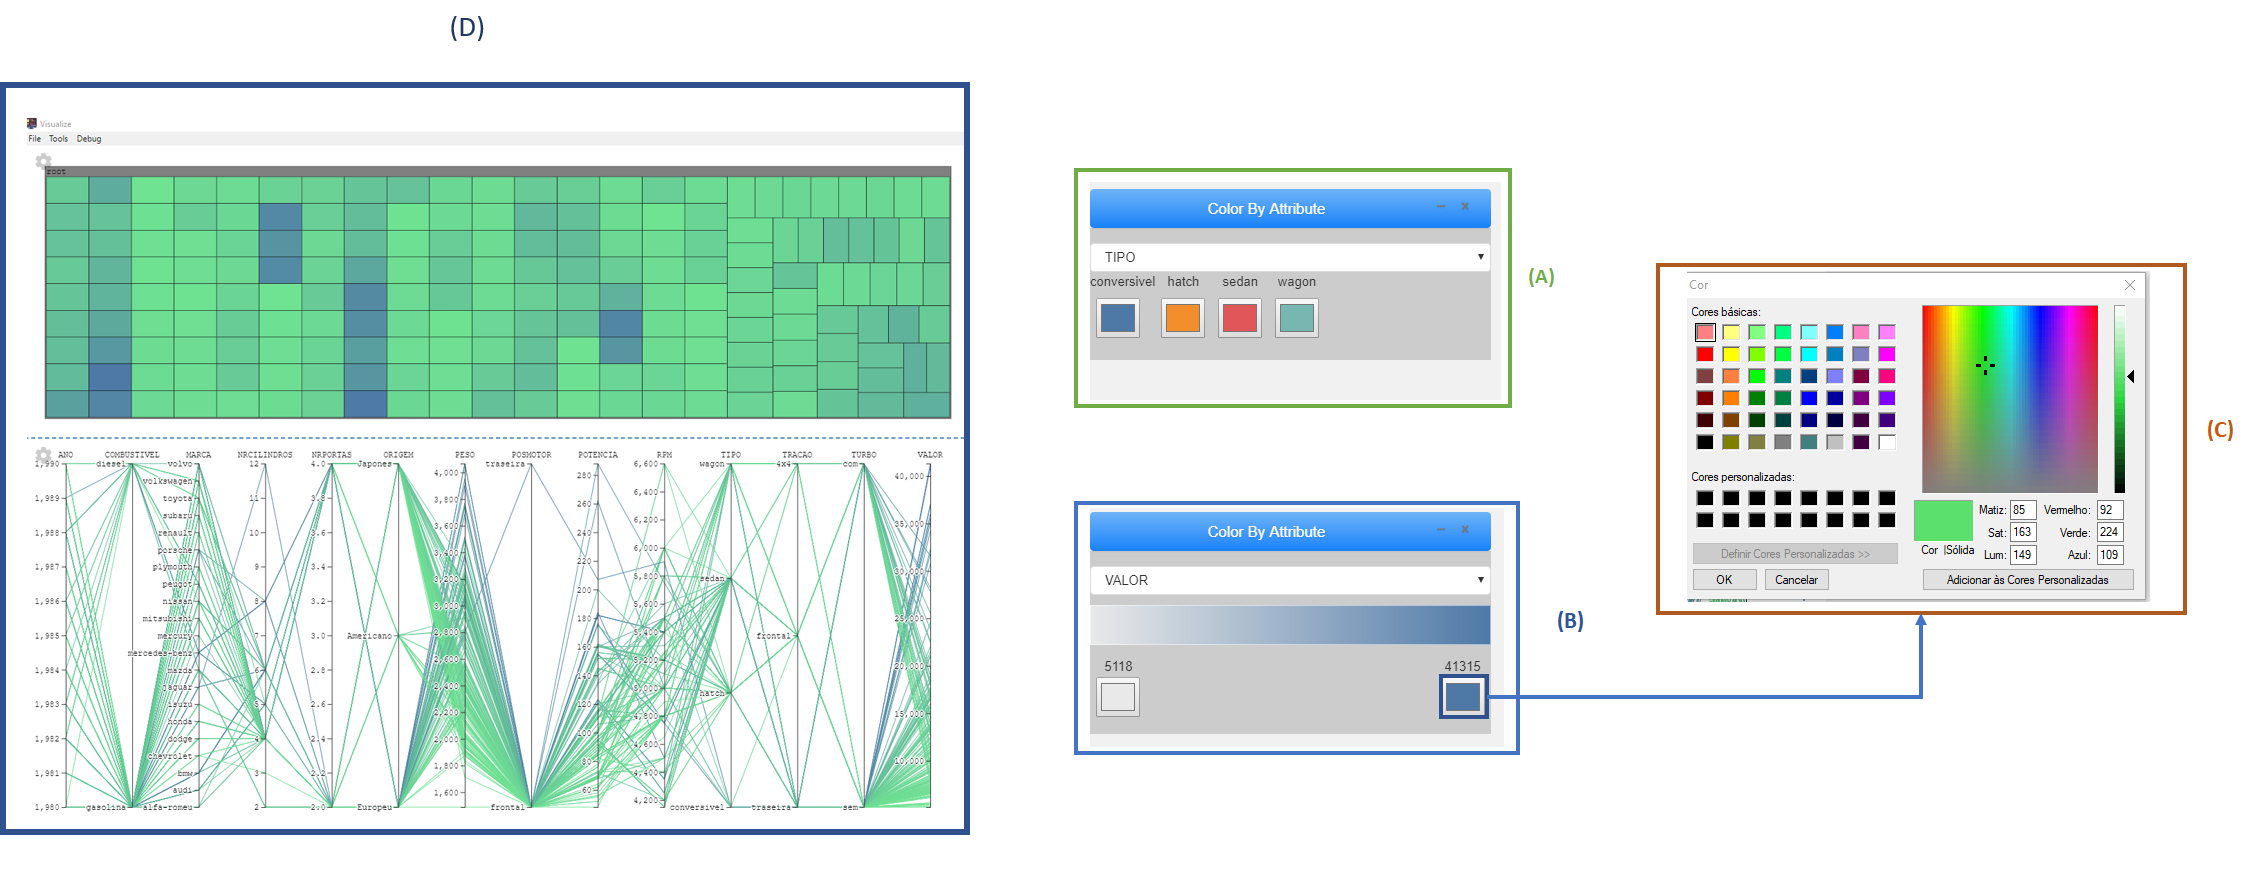
\includegraphics[width=\textwidth,scale=1]{figures/duas visualizações_2.png}
	\end{center}
	\legend{Fonte: O autor}
\end{figure}

A \autoref{fig_color_visualization} ilustra os menus de seleção de cor por atributo, onde no ponto ''(a)'' podemos ver uma seleção por atributos categóricos, na parte ''(b)'' é demonstrado o menu para atributos contínuos, e ''(c)'' o menu seletor de cores quando é selecionado um atributo. Do mesmo modo, ainda na \autoref{fig_color_visualization} no item ''(d)'' podemos ver duas visualizações utilizando o mesmo padrão de cores em um determinado atributo.

\subsection{Filtros e Seleção}
Na ferramenta existem dois tipos de filtros e seleções por atributo e por dimensão. Seleção e filtro por meio dos atributos tanto categóricos como contínuos. Caso seja escolhido um atributo categórico é disponibilizado um botão de seleção com as opções de cada atributo, caso o atributo seja contínuo é disponibilizado um \textit{slider} com o range entre o valor máximo e o mínimo como o exemplo da figura \autoref{fig_filtro_visualization}.

\begin{figure}[h]
	\caption{\label{fig_filtro_visualization} Exemplos do menu de filtro, (A) filtro menu de filtro contínuos e com um exemplo de visualização, (B) filtro menu categórico e visualização, (C) legenda menu de legenda de cores.
}
	\begin{center}
	    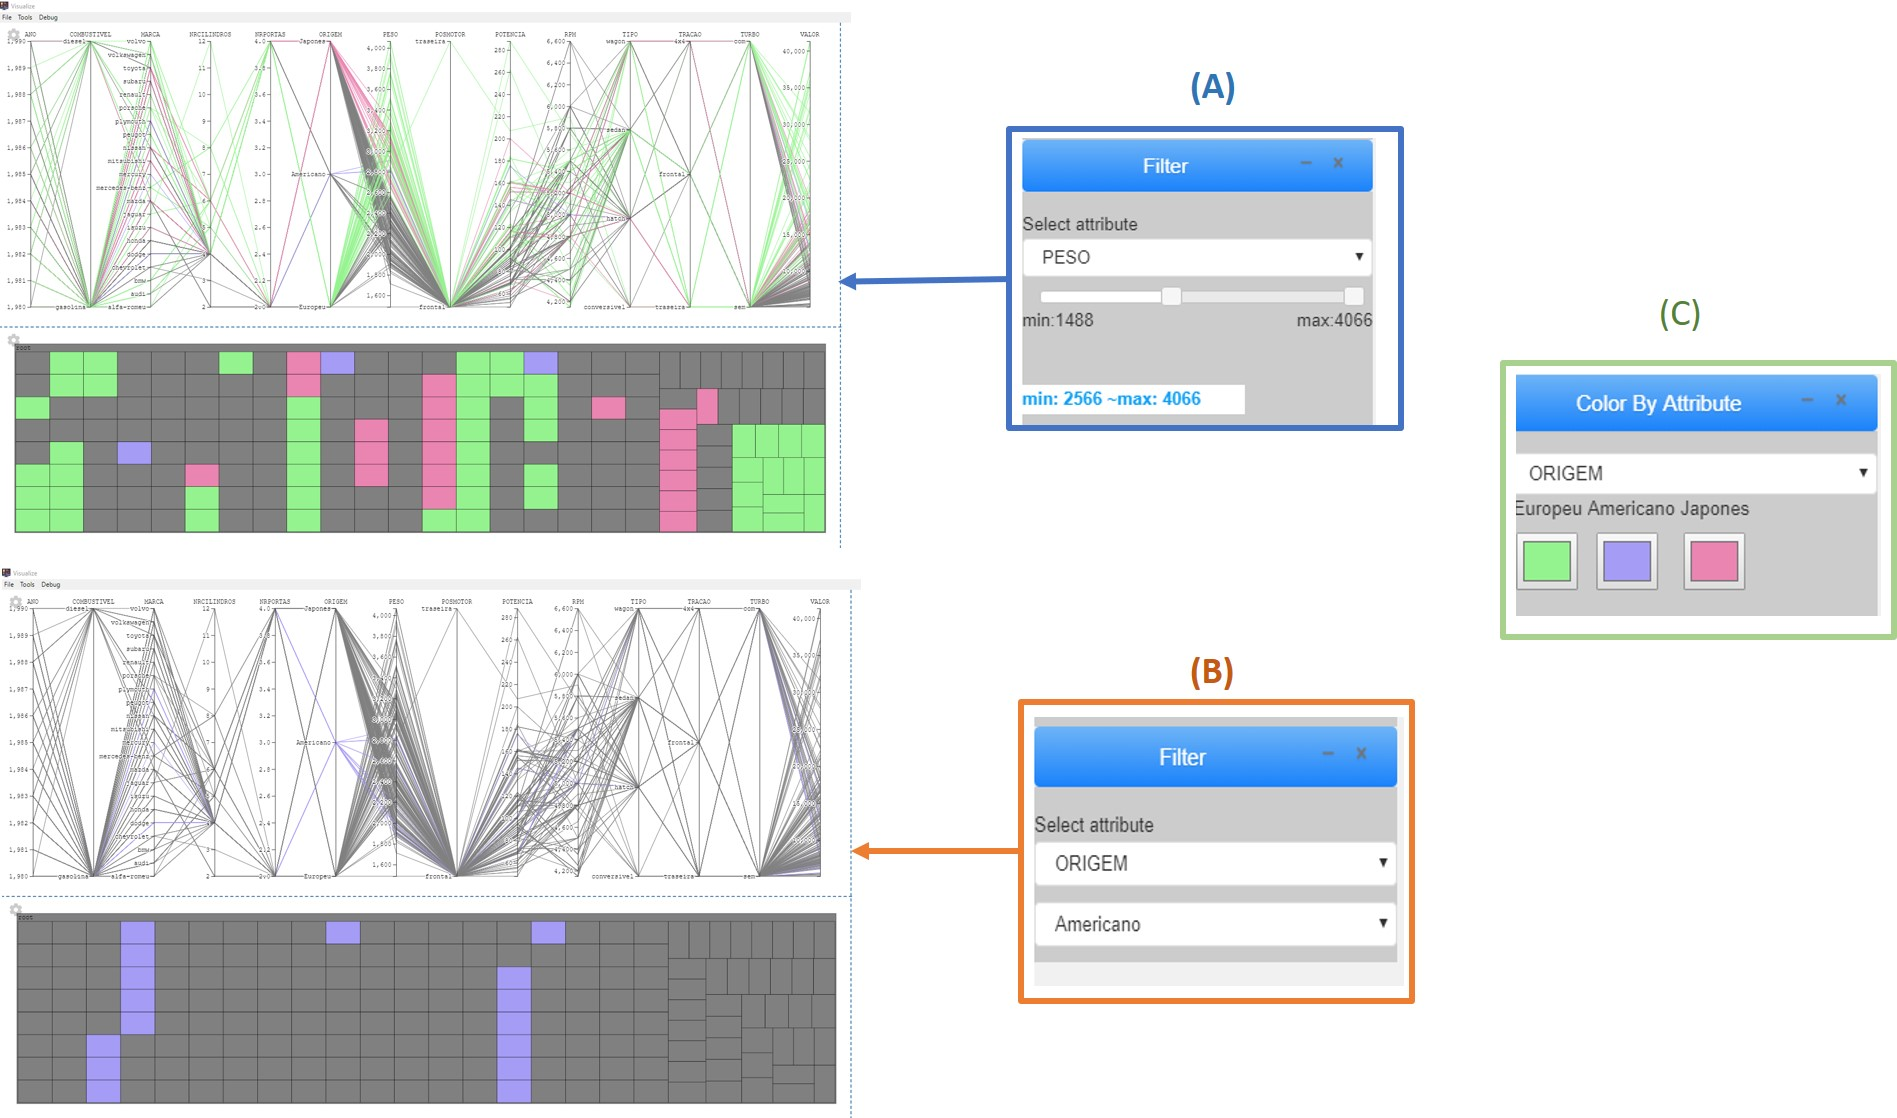
\includegraphics[width=\textwidth]{figures/filtro.jpg}
	\end{center}
	\legend{Fonte: O autor}
\end{figure}

O filtro por dimensão dos dados pode ser utilizado em visualizações como \textit{scatterplot}, \textit{barchart}, \textit{histograma}, para dados multivariados foi implementado um filtro em uma dimensão de dados; no caso reduzindo um eixo ou parte da visualização correspondente a respectiva coluna da base de dados, reduzindo a visualização e dando maior ênfase nas partes de interesse como ilustrado na \autoref{fig_filtro_dimension_visualization}.

\begin{figure}[h]
	\caption{\label{fig_filtro_dimension_visualization} Exemplos do menu de filtro, (A) menu de filtro por dimensões e fluxo com filtro realizado nas visualizações deixando apenas 4 dimensões.
}
	\begin{center}
	    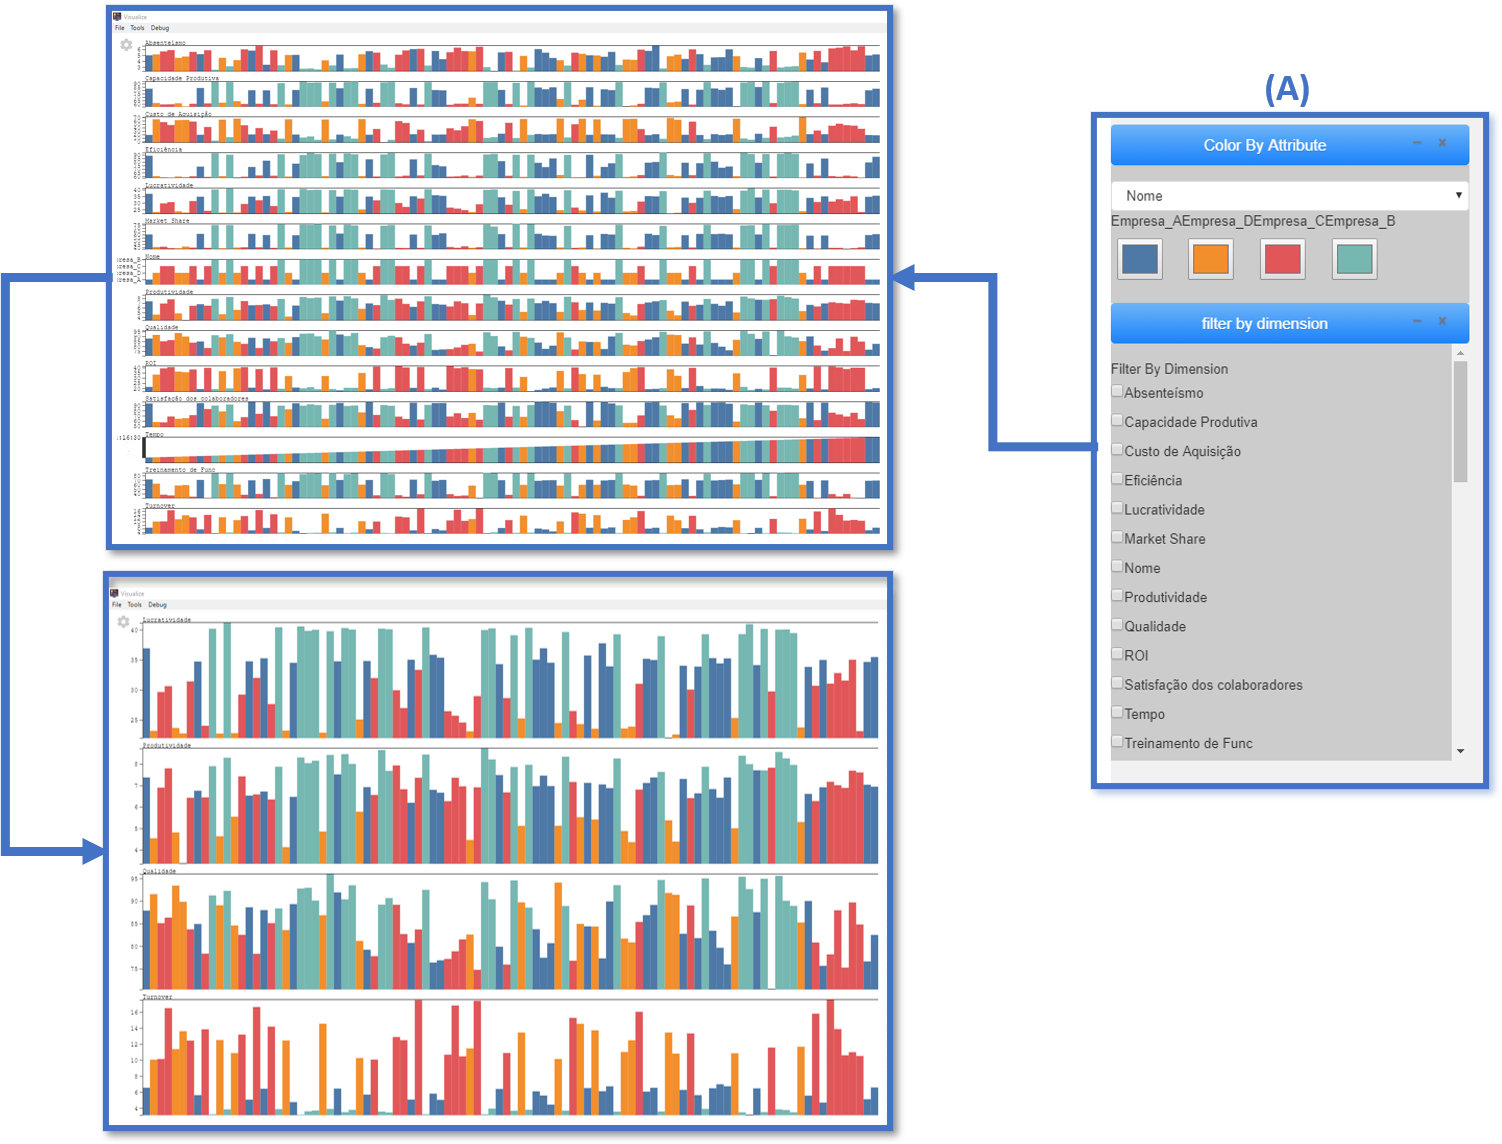
\includegraphics[width=\textwidth]{figures/filtro_dimensao.png}
	\end{center}
	\legend{Fonte: O autor}
\end{figure}


\subsection{Criação de Hierarquias}
O Controle de hierarquias pode ser feito em visualizações hierárquicas como \textit{treemap}, \textit{cicle packing}, e \textit{sunburst}, a ferramenta permite adicionar, remover estruturas hierárquicas nos dados, e decidir a ordem das hierarquias e também decidir qual atributo definirá o tamanho de cada item, como pode ser visualizado na figura \autoref{vis_hierarquies}. 


\begin{figure}[h]
	\caption{\label{vis_hierarquies} Exemplo de visualizações hierárquicas na ferramenta. (A) representa menu de hierarquias onde podem ser selecionadas conforme os dados e definida a ordem, e o \textit{size} onde se define o tamanho dos itens nas visualizações. (B) representa o atributo selecionado para as core na visualização.
}
	\begin{center}
	    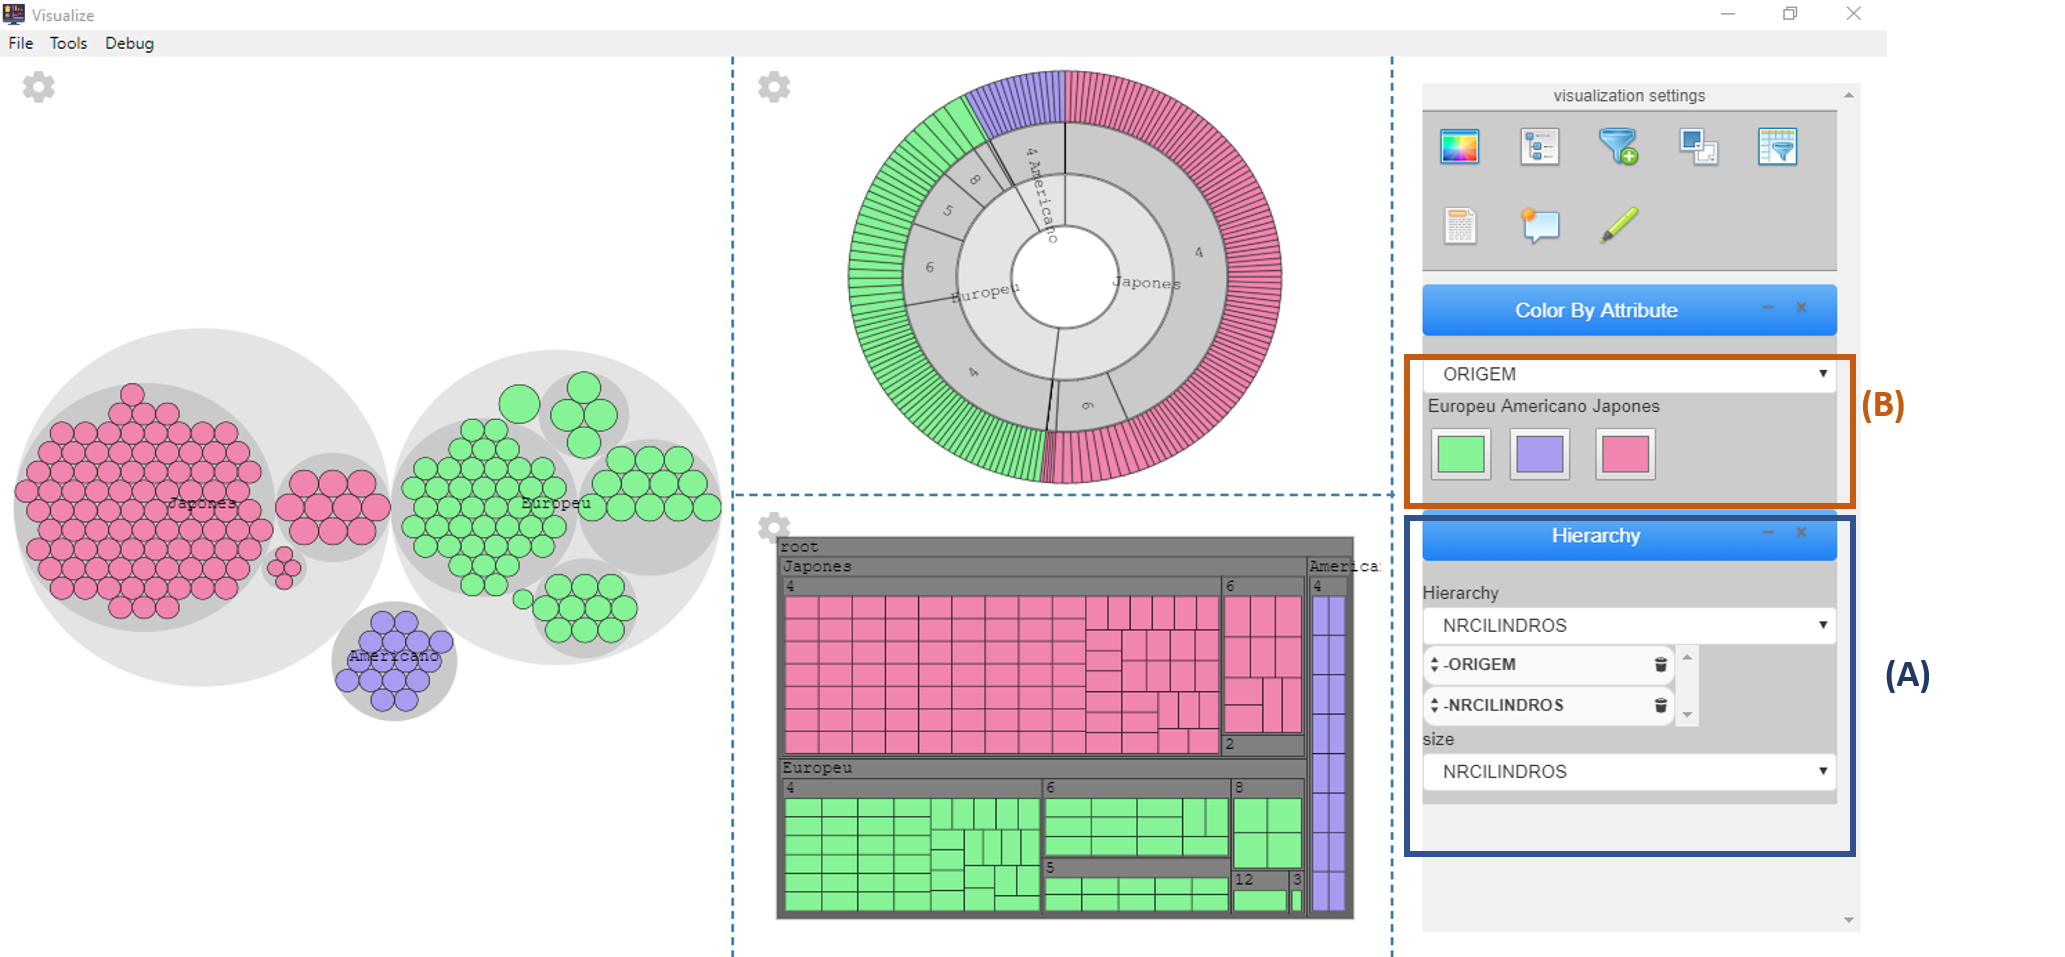
\includegraphics[width=\textwidth,scale=1]{figures/hierarquias.png}
	\end{center}
	\legend{Fonte: O autor}
\end{figure}

\subsection{Detalhes sobre Demanda}
Interação de detalhes sobre demanda configurável quando mouse é passado sobre o item, a ferramenta permite selecionar quais dimensões serão visualizadas no \textit{tooltip} de detalhes sobre demanda.

\subsection{Destaque}
Por meio de seleção do mouse e clique ou passagem do mouse de maneira coordenadas nas visualizações, por exemplo, em caso de várias visualizações no \textit{dashboard}, o mesmo item será destacado nos diferentes a gráficos. A \autoref{vis_destaque} ilustra essa situação.
\begin{figure}[h]
	\caption{\label{vis_destaque} Exemplo de duas visualizações com destaque no item de maneira coordenada.
}
	\begin{center}
	    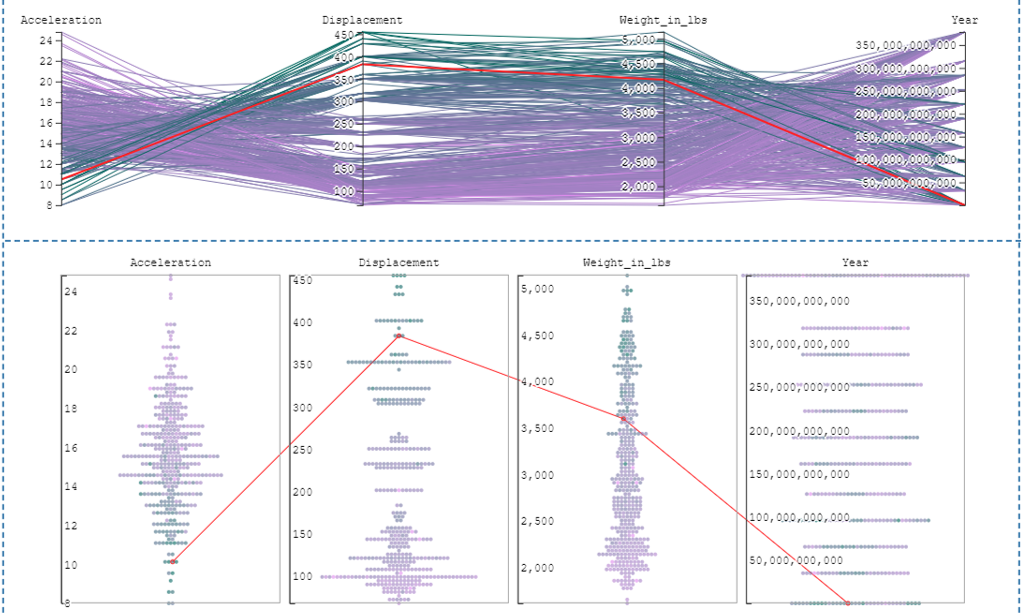
\includegraphics[width=35pc,scale=1]{figures/cordinate_highliht.png}
	\end{center}
	\legend{Fonte: O autor}
\end{figure}

\subsection{Anotações}
Interação de anotações sobre os itens da base de dados, podendo ser personalizadas, exemplo \autoref{vis_anotacao}.

\begin{figure}[h]
	\caption{\label{vis_anotacao} Exemplo de anotações no beeswarmplot.
}
	\begin{center}
	    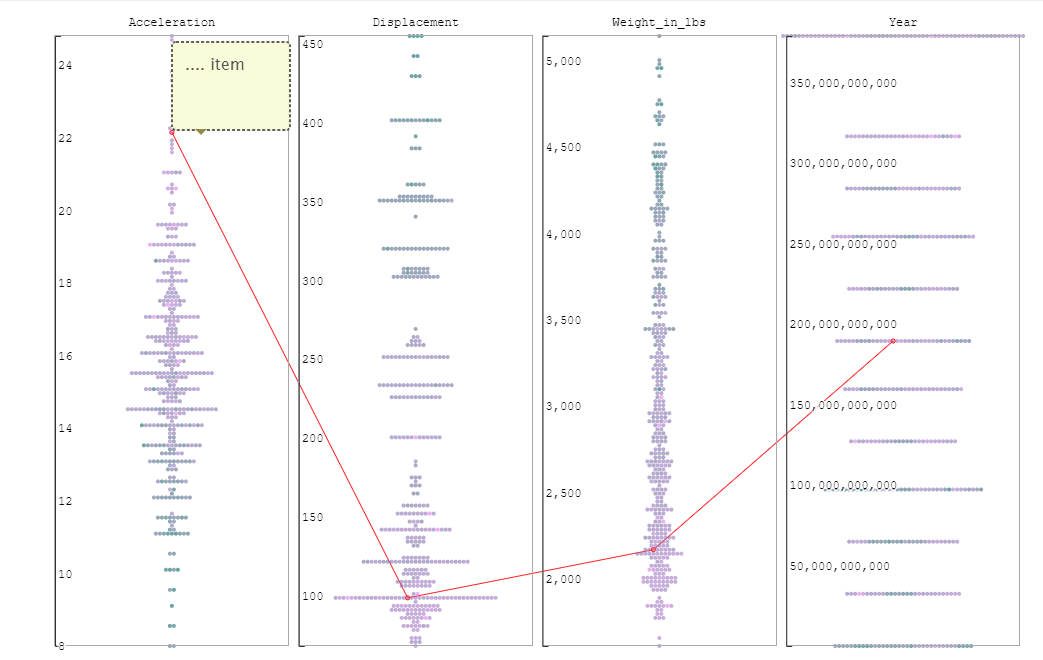
\includegraphics[width=35pc,scale=1]{figures/anottation.png}
	\end{center}
	\legend{Fonte: O autor}
\end{figure}
\chapter{Criação de \textit{dashboards} flexíveis} 
\label{ch:dashboardsflexíveis}
A criação das divisões de tela para a geração das dos \textit{dashboards} são feitas com base no \textit{layout flex-box} definido em \cite{w3c}
como um modulo de criação de \textit{layout} disponível no CSS permitindo, flexibilidade facilitando a criação uma estrutura responsiva baseada em direcionamentos de linhas e colunas, sem utilizar os de outras propriedades de posicionamento ou definir o posicionamento manualmente.
Utilizando esse objeto JSON é possível gerar as divisões de telas e armazenar a informação das visualizações já presentes na \autoref{exemplo_json} segue um exemplo resumido do objeto JSON desenvolvido.

\begin{figure}
	\caption{\label{exemplo_json}
	Estrutura de dados presente nos arquivos JSON para criação das divisões de tela. O trecho de código contém as propriedades \textit{id} , \textit{direction}  \textit{proportion},  \textit{isLeaf} , \textit{children} , \textit{content} disponíveis nos layouts de tela.
	}
	\begin{center}
	    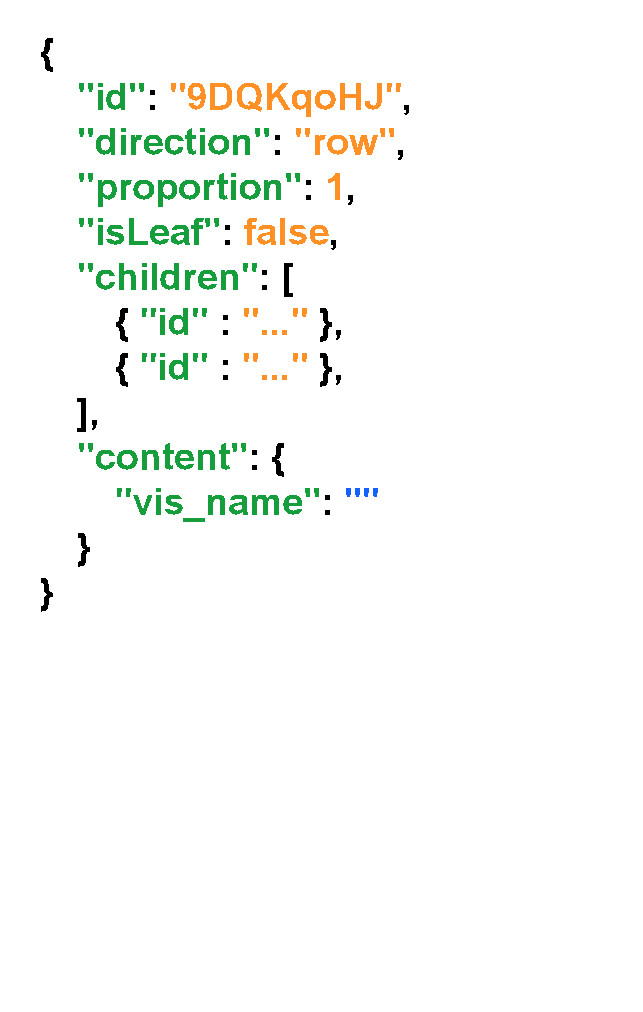
\includegraphics[width=\textwidth/3,size=0.5,trim={0mm 65mm, 20mm 0mm}]{figures/jsonFormat.pdf}
	\end{center}
	\legend{Fonte: O autor}
\end{figure}

Os seguintes atributos descritos  no arquivo JSON na \autoref{exemplo_json} servem como base para a criação dos \textit{dashboards}, o atributo (\textit{id}) é a indicação de referência para o HTML, o atributo (\textit{parent}) se refere a partição para pai e apenas se for \textit{root} não e referenciada, o atributo (\textit{proportion}) tem como objetivo armazenar a proporção da partição em relação ao total variando em número entre 0 e 1, o atributo (\textit{isLeaf}) é um booleano indicando se é folha ou não na árvore de estrutura JSON, o atributo (\textit{html}) referência do elemento HTML renderizado em tela, o atributo (\textit{content}) representa o conteúdo contido nessa divisão, e o atributo (\textit{vis-name}) contém o nome do da visualização que será gerada pelo protótipo.

Outro atributo importante é o (\textit{direction}) a direção que pode ser referenciada como linha \textit{row} para divisões horizontais ou colunas \textit{column} para divisões verticais. O atributo (\textit{children}) visa criar as subdivisões tanto verticais quanto horizontais, adicionando um novo objeto com todos os atributos de partições e dentro dessas partições podem conter o atributo \textit{children} com novas hierarquias de subdivisões. segue abaixo alguns trechos de código e das partições e suas respectivas telas geradas pela aplicação. 

Para realizar a geração das visualizações caso a partição seja um nó folha pode ser adicionada um conteúdo HTML por padrão e colocado um \textit{button} HTML para adicionar uma nova visualização ou no caso já esteja adicionado um conteúdo e selecionada o nome da visualização gerada pela biblioteca de gráficos quando importado a base de dados.

\section{ \textit{Layouts} de tela} 
Nesta seção serão exemplificados alguns arquivos JSON para criação te telas os quais são gerados por uma ferramenta de recorte na aplicação sem necessidade de trabalhar diretamente no arquivo JSON, com base nesse arquivo a mesma estrutura pode ser utilizada para salvar o estado do \textit{dasboard} na aplicação e também pode servir como um layout para diferentes bases de dados.

\section{Exemplo de \textit{layout horizontal} com hierarquias internas}
No trecho de código disponível na \autoref{jsonLayout} podemos ver um JSON resumido das partições e o resultado renderizado na tela ao lado. Pode observado no arquivo JSON, o objeto principal com o \textit{id} onde em seu atributo \textit{children} existem três objetos com as direções atribuídas como linhas (\textit{row}) formado divisões horizontais que são renderizadas na tela a primeira em destaque em azul, a segunda em destaque em vermelho, e a terceira em destaque verde as mesmas cores estão respectivamente em destaque na tela ao lado do código com uma barra da com mesma cor na \autoref{jsonLayout}.
\begin{figure}[h]
	\caption{\label{jsonLayout} tela com divisões horizontais renderizadas pelo arquivo JSON. No arquivo JSON resumido e visualização da tela gerada pelo arquivo, o código tem cores para exemplificar as partições que estão presentes nos layouts e na tela uma barra da mesma cor}
	\begin{center}
	    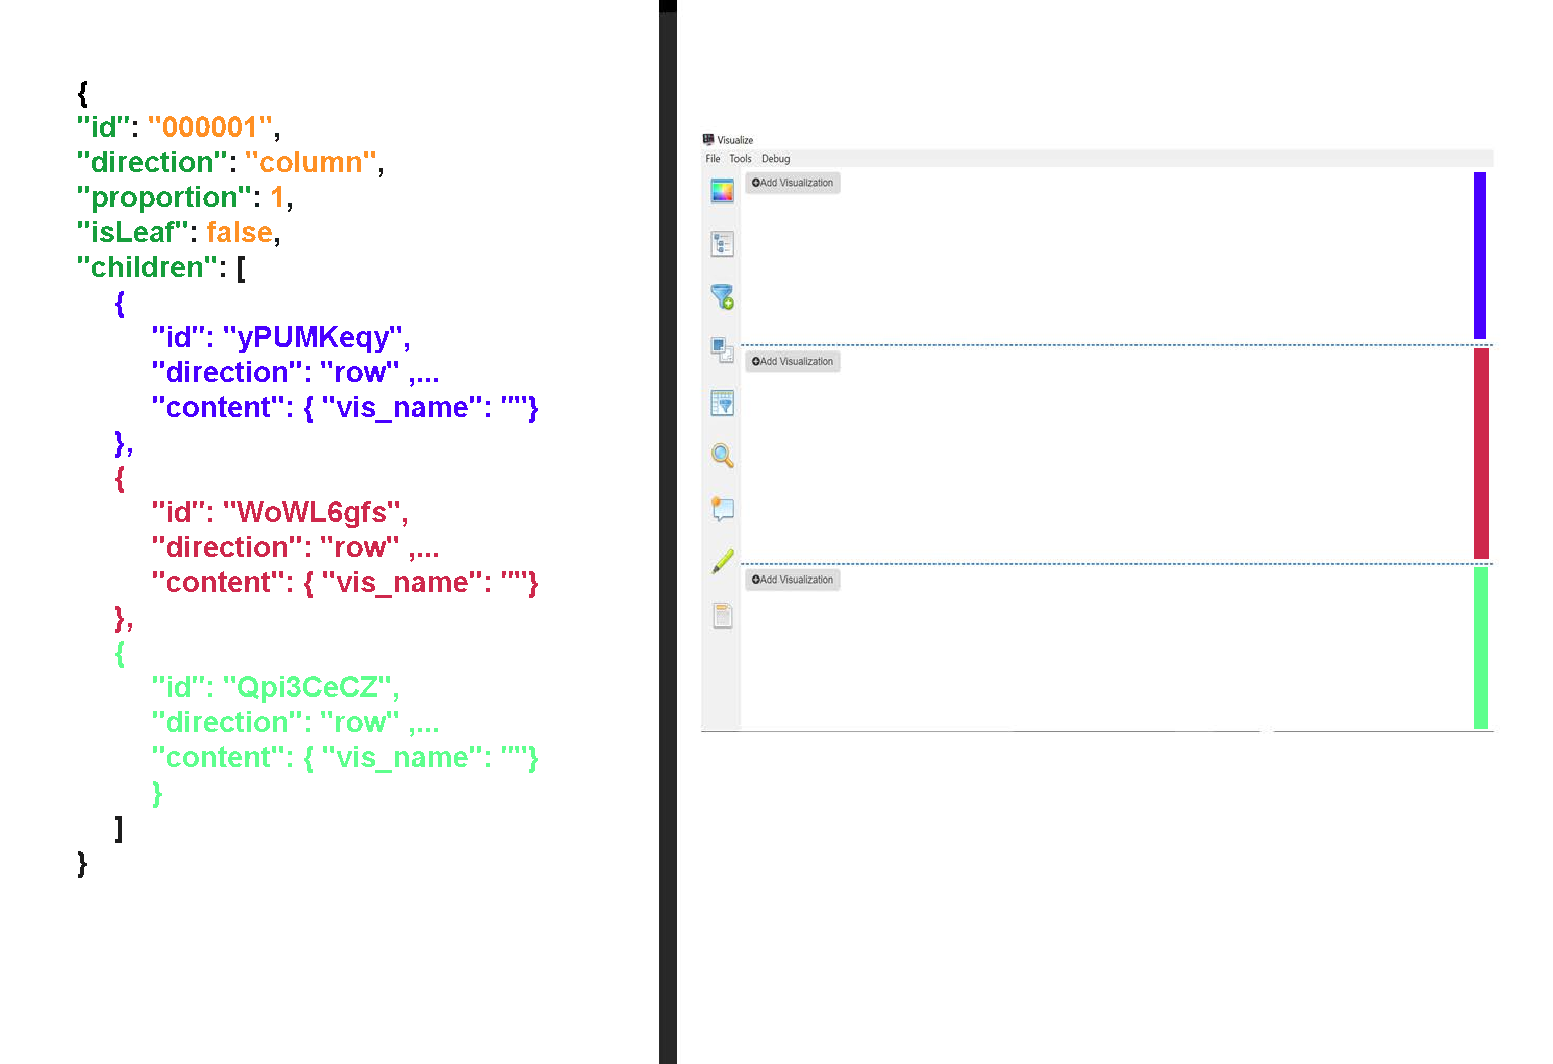
\includegraphics[width=\textwidth,trim={0mm 30mm, 0mm 0mm} ,clip]{figures/dash1_tcc.pdf}
	\end{center}
	\legend{Fonte: O autor}
\end{figure}

\section{Exemplo com divisões verticais e horizontais com 
hierarquias internas}
No trecho de código a exemplificado na \autoref{jsonLayout2} podemos ver o código resumido das partições e o resultado demonstrado em tela. No arquivo JSON resumido podemos ver o código onde existem as divisões de tela o objeto principal com (\textit{id}": ''9DQKqoHj'') contém três objetos principais os dois primeiros em cinza e vermelho são as divisões verticais com as mesmas cores respectivas nas barras da tela renderizada, o terceiro objeto contém divisões horizontais com as respectivas cores verde, azul e rosa também destacados na tela renderizada com barras na mesma cor.

\begin{figure}[h]
	\caption{\label{jsonLayout2} tela com divisões horizontais proveniente do arquivo JSON, arquivo JSON resumido e visualização da tela gerada pelo arquivo, o código tem cores para exemplificar as partições que estão presentes nos layouts e na tela uma barra da mesma cor }
	\begin{center}
	    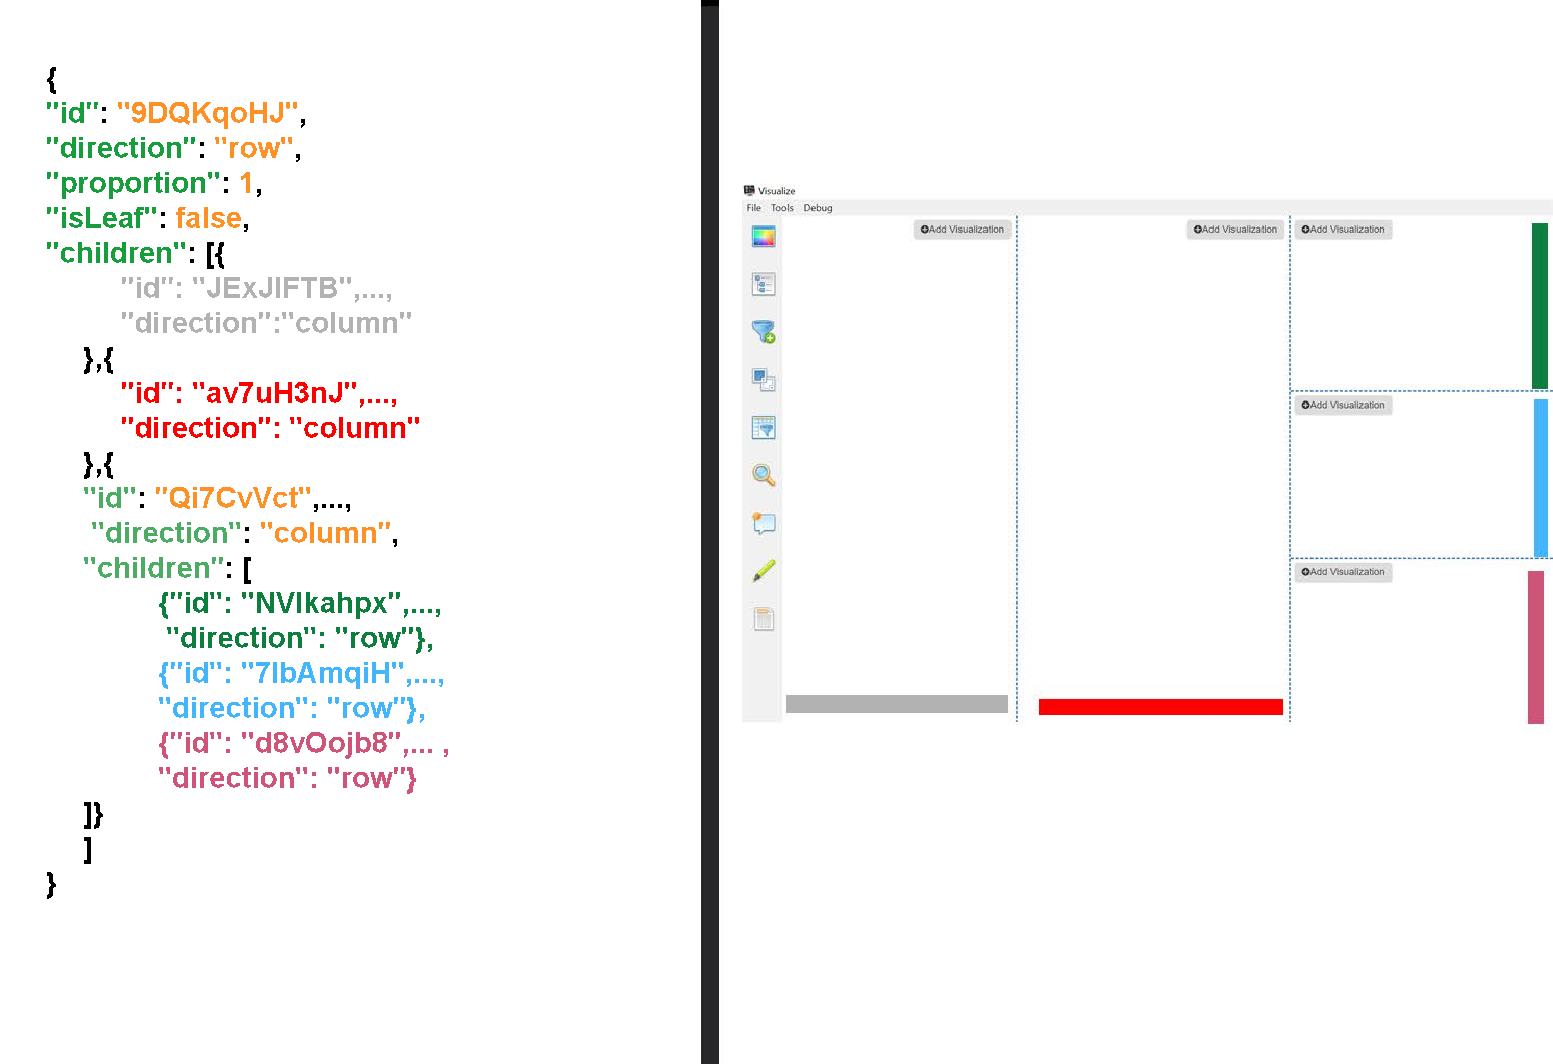
\includegraphics[width=\textwidth,trim={0mm 25mm, 0mm 0mm} ,clip]{figures/dash2_tcc.pdf}
	\end{center}
	\legend{Fonte: O autor}
\end{figure}

\section{Exemplo de \textit{dashboard} com divisões horizontais e verticais}
\begin{figure}[h]
	\caption{\label{jsonLayout3} tela com divisões e visualizações proveniente do arquivo JSON. As cores dos objetos principais em destaque no objeto JSON tem seus correspondentes na colorida na tela renderizada}
	\begin{center}
	    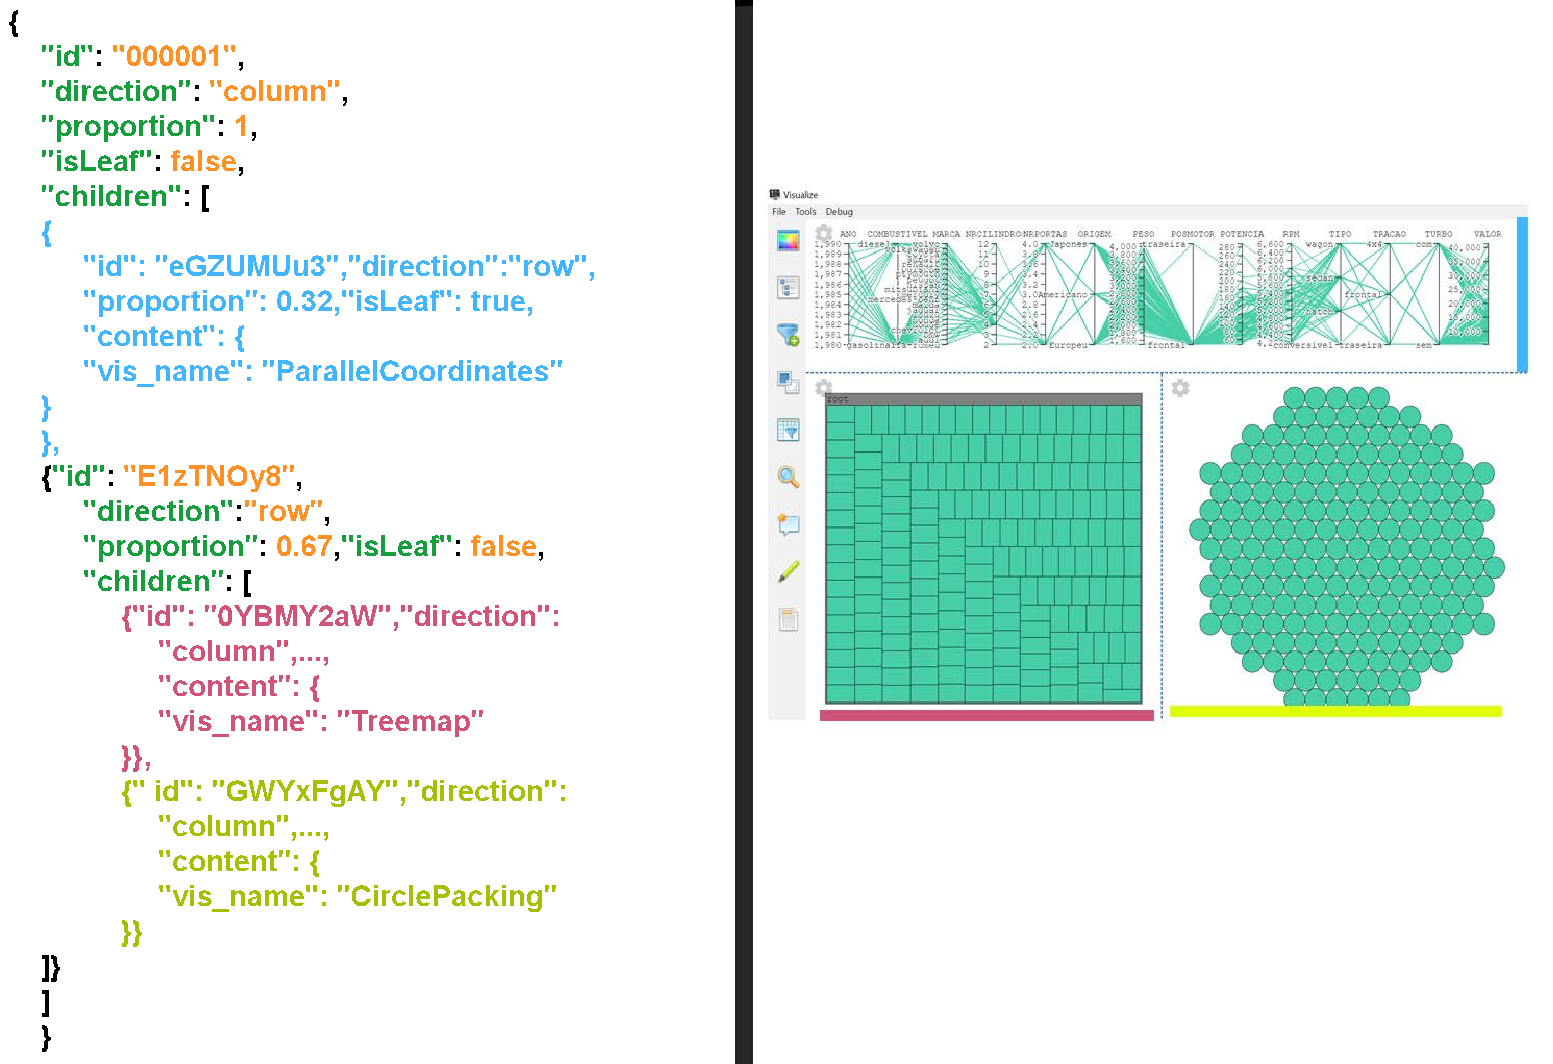
\includegraphics[width=\textwidth]{figures/dash3_tcc.pdf}
	\end{center}
	\legend{Fonte: O autor}
\end{figure}

    
Na \autoref{jsonLayout3} contém o código para geração de um \textit{dashboard} o resultado renderizado em tela do outro lado. Nesse exemplo de código JSON possui dois objetos principais, contida no objeto principal (\textit{id}:"000001") em azul temos a divisão horizontal com um gráfico de coordenas paralelas e no segundo objeto (\textit{id}:"E1zTNOy8") possui em seu atributo \textit{children} dois filhos a primeira em rosa com um \textit{treemap} e a segunda e verde com uma \textit{circle packing}.


\chapter{Caso de uso}
\label{ch:base}
Nessa seção será realizado um caso de uso utilizando a ferramenta proposta e abordando a elaboração e construção da base de dados, as perguntas a serem respondias, e as propostas de \textit{dashboards} elaboradas.


\section{Indicador-chave de desempenho - KPI}
Mckie et al. \cite{mckie2009introduction} em seu trabalho definem um indicador de desempenho como medidas quantitativas que refletem fatores sobre os objetivos da empresa, sendo pontos chaves para o sucesso organizacional. Além disso, existem diversos tipos de KPI nas empresas, como medidas de para aumentar o lucro, lucro antes de impostos, lucro por funcionário. Como benefício, esses indicadores, fornecem informações para saber o estado da empresa e focar no que realmente importa na organização.

\section{Descrição da Base}
A geração de uma base de dados sintética foi realizada na ferramenta Blocks \cite{blocks}, simulando um cenário de 4 empresas fictícias em situação de competição. Seguindo os KPI's selecionados para criação da base sintética, os atributos podem ser vistos na \autoref{tabela_indicadores}.

\begin{figure}[h]
	\caption{\label{tabela_indicadores} Indicadores Baseados nos Quadrantes do BSC (Balanced scorecard).
}
	\begin{center}
	    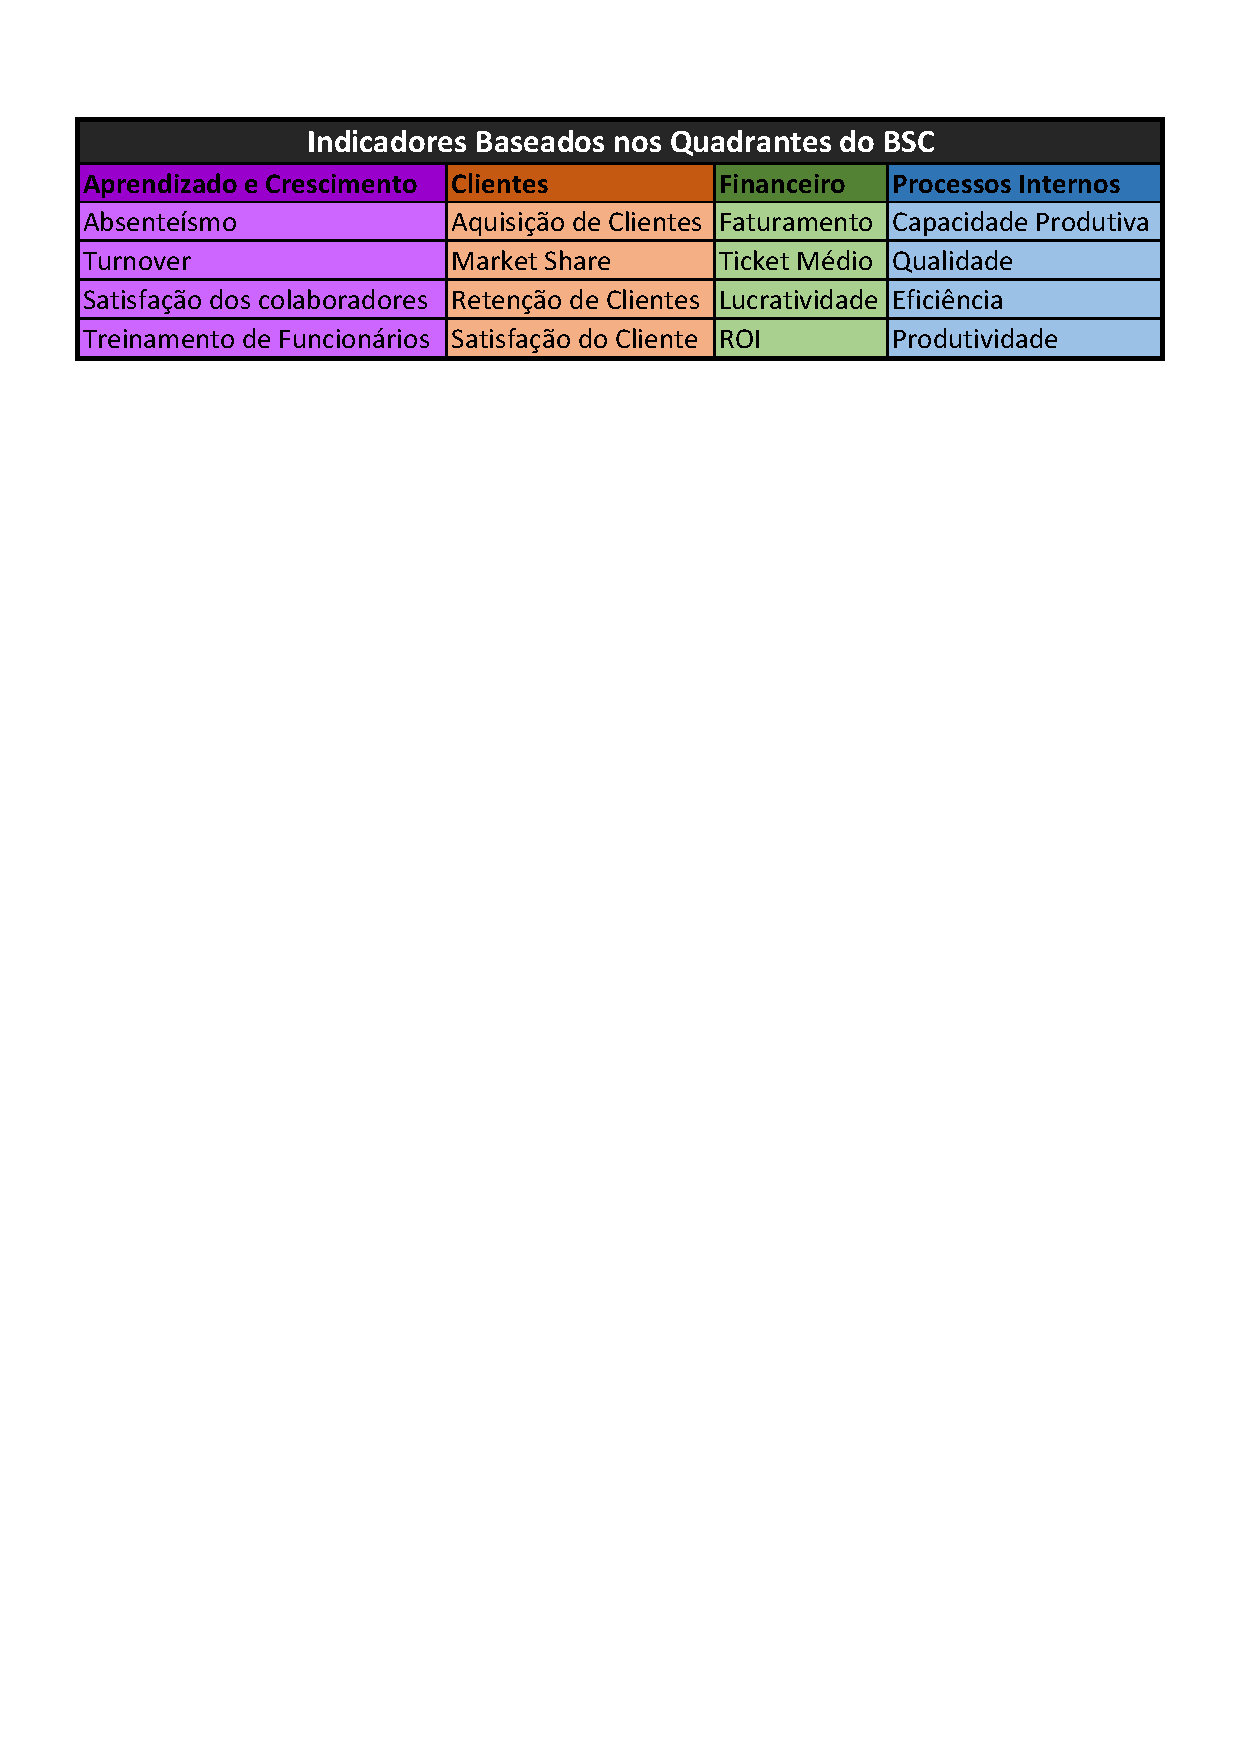
\includegraphics[width=\textwidth,scale=1,trim={0cm 230mm, 0mm 20mm},clip]
	    {figures/Indicadores - BSC.pdf}
	\end{center}
	\legend{Fonte: O autor}
\end{figure}


A elaboração da base de dados foi realizada com base no \textit{Balanced Score Card} (BSC) proposto por \cite{kaplan2000balanced}, um método feito para implementar e gerenciar organizações, com perspectivas nos seguintes setores aprendizado e crescimento, clientes , financeiro ,  processos internos , a  fornecendo medidas que permitam as organizações alcancem seus objetivos.

Dentro dos indicadores dos Processos Internos, temos a Produtividade (PRO). Este indicador representa a produtividade da equipe medida a partir das horas trabalhadas e o tamanho da atividade ou do produto desenvolvido. Como o próprio nome informa, o objetivo estratégico associado a este indicador é o aumento da produtividade da equipe. As metas e limites utilizados como métrica de medição foram:

\begin{itemize}
\item  \textbf{\textit{OK}}: acima de 8Pts/H;
\item  \textbf{\textit{Alerta}}: entre 6 e 8Pts/H;
\item  \textbf{\textit{Crítico}}: abaixo de 6Pts/H.
\end{itemize}

Neste caso, utilizaram-se Pontos (Pts) para representar o tamanho de atividades ou produtos, mas isso deve ser adaptado para realidade de cada organização. Pensou-se em um contexto em que a produtividade máxima seria representada por 10pts produzidos em uma hora. A fórmula que melhor representa a medida é: $PRO = Pts/H$. Onde (Pts) são os pontos da tarefa e (H) as horas utilizadas para executar a tarefa, utilizando decimal como unidade de medida.

A Capacidade Produtiva (CAP) é o próximo indicador nos Processos Internos. Onde representa a capacidade máxima que a organização pode produzir em um período com os recursos que tiver à sua disposição. O objetivo estratégico associado é saber se a empresa consegue atender adequadamente à demanda solicitada por seus clientes. Ou ainda, se precisará realizar algum ajuste. Seja no quadro de funcionários ou processos, caso a capacidade esteja muito acima ou abaixo em relação à demanda. As metas e limites utilizados como métrica serão:
\begin{itemize}
\item  \textbf{\textit{OK}}: acima de 90\%;
\item  \textbf{\textit{Alerta}}: entre 80\% e 90\%;
\item  \textbf{\textit{Crítico}}: abaixo de 80\%.
\end{itemize}

A fórmula para representar essas metas e limites pode ser melhor descrita como CAP = (PDA/PDT), onde (PDA) é a produção atual e (PDT) a produção total, utilizando percentual como unidade de medida.

O próximo indicador apresentado nos Processos Internos é a Eficiência (EFC). Representa a capacidade de produzir mais consumindo menos recursos. Onde o seu objetivo estratégico associado é conseguir o melhor rendimento com o mínimo de erros e/ou dispêndios. As metas e limites indicados são:
\begin{itemize}
\item  \textbf{\textit{OK}}: acima de 85\%;
\item  \textbf{\textit{Alerta}}: entre 70\% e 85\%;
\item  \textbf{\textit{Crítico}}: abaixo de 70\%.
\end{itemize}

A fórmula apresentada é $EFC = PDE/PDP$, onde (PDE) é a produção efetiva e (PDP) é a produção planejada, utilizando também o percentual como unidade de medida.

Por fim, temos a Qualidade (QUA) como o último indicador dos Processos Internos. Onde apresenta um conceito subjetivo, porém de maneira geral é o grau de excelência do que é entregue como produto ou serviço, estando conforme e consistente com as expectativas dos clientes e em conformidade com normas e requisitos funcionais, adequado à finalidade para a qual foi projetado. Tendo como foco do objetivo estratégico aumentar a qualidade dos produtos/serviços entregues. As metas e limites serão representados por: 
\begin{itemize}
\item  \textbf{\textit{OK}}: maior ou igual a 95\% dos defeitos identificados antes de o projeto ser entregue ao cliente;
\item  \textbf{\textit{Alerta}}: entre 80\% e 94,9\% dos defeitos identificados antes de o projeto ser entregue ao cliente;
\item  \textbf{\textit{Crítico}}: abaixo de 79,9\% dos defeitos identificados antes do projeto ser entregue ao cliente.
\end{itemize}

A fórmula que melhor representa essas medidas é $QUA = TDI/(TDI+TDE) \times 100$. Onde (TDI) é o total de defeitos internos e (TDE) o total de defeitos externos. Utilizando percentual como unidade de medida.

O primeiro indicador apresentado para o quadrante Financeiro é a Lucratividade (LUC). Este indicador mede a capacidade operacional do empreendimento em gerar lucros a partir de um projeto desenvolvido. Tendo como objetivo estratégico aumentar o lucro da organização. As metas e limites definidos como métricas são representadas por:
\begin{itemize}
\item  \textbf{\textit{OK}}: acima de 25\%;
\item  \textbf{\textit{Alerta}}: entre 10\% e 25\%;
\item  \textbf{\textit{Crítico}}: abaixo de 25\%.
\end{itemize}

A fórmula que descreve essas metas e limites é LUC = (LUL/REC) \times  100. 

Onde (LUL) é o lucro líquido  e (REC) a receita total, utilizando percentual como unidade de medida.O segundo indicador do quadrante Financeiro é o Faturamento(FAT). Onde representa a soma de todas as vendas realizadas ou serviços prestados em um determinado período. Onde seu objetivo estratégico é determinar a performance de vendas, entendendo-se se o preço cobrado está dentro da expectativa dos consumidores. Apresentando as metas e limites abaixo:

\begin{itemize}
\item  \textbf{\textit{OK}}: acima de 60\% do limite de faturamento do porte da empresa;
\item  \textbf{\textit{Alerta}}: entre 40\% e 60\% do limite de faturamento do porte da empresa;
\item  \textbf{\textit{Crítico}}: abaixo de 40\% do limite de faturamento do porte da empresa.
\end{itemize}

A fórmula apresentada para descrever essas métricas é $FAT = (SVE/FPE) 	\times 100$. Onde (SVE) é a soma do valor de entrada e (FPE) o faturamento da porta da empresa. Sendo o percentual utilizado como unidade de medida.

O terceiro indicador do quadrante Financeiro é o Ticket Médio (TME). Indicando o valor gasto, em média, por cada cliente no negócio. Tendo como objetivo estratégico melhorar a performance de vendas e adequar o valor do produto/serviço fornecido. As metas e limites são apresentados por:
\begin{itemize}
\item  \textbf{\textit{OK}}: acima de 300\% do custo da aquisição por cliente;
\item  \textbf{\textit{Alerta}}: entre 150\% e 300\% do custo da aquisição por cliente;
\item  \textbf{\textit{Crítico}}: abaixo de 150\% do custo da aquisição por cliente.
\end{itemize}

A fórmula utilizadas para representar essas metas e limite é $TME = (FTP/NPP) \times 100$. Onde (FTP) é o faturamento total no período e (NPP) é o número de pedidos no período. Utilizando também o percentual como unidade de medida.

Finalizando temos com o Retorno sobre Investimento(ROI) como quarto indicador do quadrante Financeiro. Retorno sobre investimento (em inglês, return on investment ou ROI), também chamado taxa de retorno, taxa de lucro ou simplesmente retorno, é a relação entre a quantidade de dinheiro ganho (ou perdido) como resultado de um investimento e a quantidade de dinheiro investido. Seu objetivo estratégico é aumentar o retorno em relação ao investimento. As metas e limites são apresentados por:
\begin{itemize}
\item  \textbf{\textit{OK}}: acima de 20\%;
\item  \textbf{\textit{Alerta}}: entre 30\% e 40\%;
\item  \textbf{\textit{Crítico}}: abaixo de 40\%.
\end{itemize}

A fórmula que representa as métricas apresentadas acima é $ROI = (REC - CUS) CUS	\times 100$. Onde (REC) é a receita e (CUS) o custo. O percentual também é unidade de medida utilizada. 

O primeiro indicador do quadrante Clientes é a Satisfação do Cliente(SCL). Apresentando o sentimento de prazer ou de desapontamento resultante da comparação do desempenho esperado pelo produto (ou resultado) em relação às expectativas da pessoa. O objetivo estratégico associado a esse indicador foca em aumentar a satisfação dos clientes. As metas e limites podem ser medidos como:
\begin{itemize}
\item  \textbf{\textit{OK}}: acima de 90\%;
\item  \textbf{\textit{Alerta}}: entre 70\% e 90\%;
\item  \textbf{\textit{Crítico}}: abaixo de 70\%.
\end{itemize}

A fórmula que melhor descreve essas métricas é $SCL = SPS/NPR$. Onde (SPR) é o somatório do percentual de satisfação e (NPR) o número de pesquisas respondidas. Utilizando o percentual como unidade de medida.

O segundo indicador do quadrante Clientes é o Custo de Aquisição por Clientes(CAC). O Custo de Aquisição de Clientes (CAC) é um dos principais indicadores de vendas usado por empresas para medir o quanto custa conquistar um cliente. O CAC inclui desde custos de marketing até os salários e comissões dos vendedores que atuam ativamente na venda de uma solução, produto ou serviço. O objetivo estratégico é otimizar a relação custo benefício de aquisição e retorno de clientes. As metas e limites podem ser apresentados por:
\begin{itemize}
\item  \textbf{\textit{OK}}: abaixo de 33\% do valor do ticket médio;
\item  \textbf{\textit{Alerta}}: entre 33\% e 66\% do valor do ticket médio;
\item  \textbf{\textit{Crítico}}: acima de 66\% do valor do ticket médio.
\end{itemize}

Essas metas e limites são representadas pela fórmula $CAC = (SOI/NCA) 	\times 100$. Onde (SOI) é a soma dos investimentos e (NCA) o número de clientes adquiridos. A unidade de medida utilizada também pelo percentual.

O terceiro indicador do quadrante Clientes é a Retenção de Clientes (RTC). Onde se caracteriza pelas ações relacionadas para reduzir o número de perdas de clientes. Visa manter o máximo de clientes ativos. As metas e limites são definidos como:
\begin{itemize}
\item  \textbf{\textit{OK}}: acima de 65\%;
\item  \textbf{\textit{Alerta}}: entre 40\% e 65\%;
\item  \textbf{\textit{Crítico}}: abaixo de 40\%.
\end{itemize}

A fórmula que melhor representa essas métricas é $RTC = (CLA/TOC) 	\times 100$. Onde (CLA) são os clientes ativos e o (TOC) o total de clientes. Utilizando também o percentual como unidade de medida.

O quarto e último indicador do quadrante Clientes é o Market Share (MKS). Este indicador se refere à participação no mercado em relação a aspectos como volume de vendas, faturamento, quantidade de clientes, lucratividade, etc. Seu objetivo estratégico é intensificar a participação no mercado. Podemos definir as metas e limites como:
\begin{itemize}
\item  \textbf{\textit{OK}}: acima de 20\%;
\item  \textbf{\textit{Alerta}}: entre 8\% e 20\%;
\item  \textbf{\textit{Crítico}}: abaixo de 8\%.
\end{itemize}

A fórmula para representar as métricas declaradas é $MKS = (REO/RTM) \times 100$. Onde (REO) é o resultado específico da organização e (RTM) o resultado total do mercado. Utilizando o percentual como unidade de medida.

O primeiro indicador do quadrante Aprendizado e Crescimento é o Turnover (TUR). Este indicador é responsável por medir a quantidade de colaboradores desligados/admitidos de uma empresa em relação ao número de colaboradores no quadro funcional. Seu objetivo estratégico associado é reter talentos a fim de manter o capital intelectual na organização. As metas e limites foram definidos por:
\begin{itemize}
\item  \textbf{\textit{OK}}: abaixo de 5\%;
\item  \textbf{\textit{Alerta}}: entre 5\% e 10\%;
\item  \textbf{\textit{Crítico}}: acima de 20\%.
\end{itemize}

Sua fórmula pode ser representada por $TUR = (MAD/NFI) 	\times 100$. Onde (MAD) é a média de admissões e desligamentos e (NFP) o número de funcionários do início do período. Percentual também é sua unidade de medida.

O segundo indicador do quadrante Aprendizado e Crescimento é o Treinamento de Funcionários (TRF). O indicador visa medir a eficiência da educação corporativa. Seu objetivo estratégico é melhorar a capacitação dos colaboradores da organização. Suas metas e limites foram representados por:
\begin{itemize}
\item  \textbf{\textit{OK}}: acima de 70\%;
\item  \textbf{\textit{Alerta}}: entre 50\% e 70\%;
\item  \textbf{\textit{Crítico}}: abaixo de 50\%.
\end{itemize}
 
A fórmula que representa os valores das metas e limites é $TRF = (TRR/TRP) 	\times 100$. Onde (TRR) são os treinamentos realizados e o (TRP) os treinamentos planejados. Utilizando o percentual como unidade de medida.

O terceiro indicador do quadrante Aprendizado e Crescimento é a Satisfação dos Colaboradores (SCO). Tal indicador refere-se ao nível de felicidade, satisfação e motivação dos colaboradores em seus trabalhos. Seu objetivo estratégico é aumentar a satisfação e motivação dos colaboradores em trabalhar na organização. Suas metas e limites são definidos por: 
\begin{itemize}
\item  \textbf{\textit{OK}}: acima de 90\%;
\item  \textbf{\textit{Alerta}}: entre 70\% e 90\%;
\item  \textbf{\textit{Crítico}}: abaixo de 70\%.
\end{itemize}

A fórmula que melhor representa essas métricas é $SCO = SPS/NPR$. Onde (SPR) é o somatório do percentual de satisfação e (NPR) o número de pesquisas respondidas. Utilizando o percentual como unidade de medida.

O quarto e último indicador do quadrante Aprendizado e Crescimento é o Absenteísmo (ABS). Absenteísmo no trabalho ou ausentismo é um padrão de falta dos funcionários por motivos que não doenças, desemprego ou licença. Seu objetivo estratégico é eliminar e/ou manter baixo o índice de absenteísmo na organização. As metas e limites definidos são:
\begin{itemize}
\item  \textbf{\textit{OK}}: até 5\%;
\item  \textbf{\textit{Alerta}}: entre 5\% e 10\%;
\item  \textbf{\textit{Crítico}}: acima de 10\%.
\end{itemize}

A fórmula que representa os valores obtidos para essas métricas é $ABS = (NHP/THT) 	\times 100$. Onde (NHP) é o número de horas perdidas e o (THT) o número de horas totais que deveriam ser executadas. Utilizando também o percentual como unidade de medida.
\autoref{resumo_Indicadores}

\begin{figure}[h]
	\caption{\label{resumo_Indicadores} Tabela de resumo de indicadores selecionados para a base de dados com as colunas KPI, as colunas de delimitações de OK, Alerta, Critíco e Unidade média
}
	\begin{center}
	    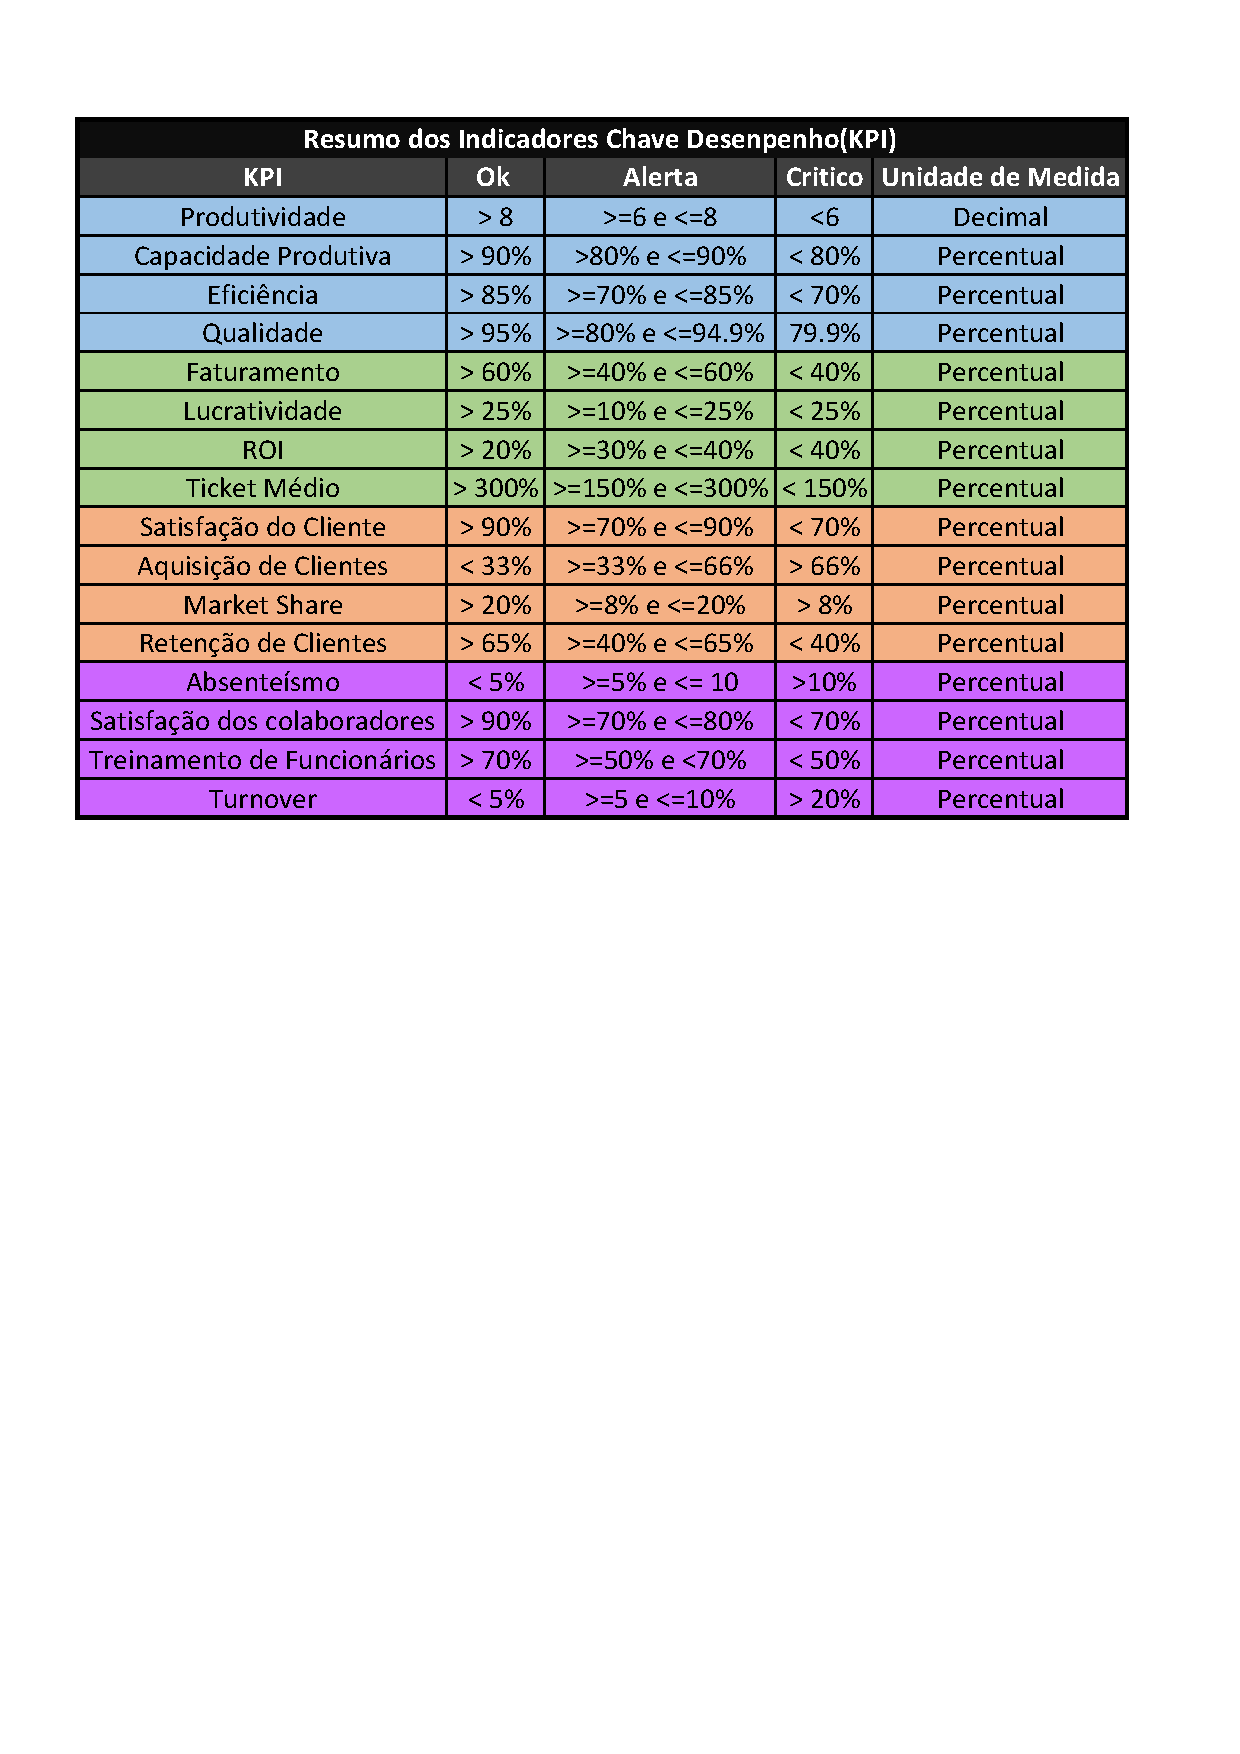
\includegraphics[width=\textwidth,trim={0cm 155mm, 0mm 20mm},clip]{figures/resumoIndicadores- BSC.pdf}
	\end{center}
	\legend{Fonte: O autor}
\end{figure}


\section{Construção da Base}
A construção de uma base de dados sintética foi realizada para o caso e gerar visualizações na ferramenta, no contexto de empresas em concorrência. 
Os geradores de dados para criação da base sintética de dados selecionados no Blocks foram divididos em 4 tipos, Processos Internos, Financeiro, Clientes, Aprendizado e Crescimento.
O atributo “nome” foi selecionado do tipo ''categorical'' criando uma coluna para definir qual a empresa pertencente, no caso foram definidas como \textbf{''empresaA''}, \textbf{''empresaB''},  \textbf{''empresaC''}, \textbf{''empresaD''}.

Os demais atributos numéricos foram gerados seguindo mesmo padrão, foi selecionado o gerador \textit{''categorical Function''} onde permite selecionar um atributo categórico e para cada tipo de valor categórico contido nessa coluna gerar um numérico diferente variando entre \textit{''Gaussian Generator''} um gerador que cria valores em uma gaussiana entre um determinado intervalo e \textit{''Uniform Generator''} que gera valores uniformes aleatoriamente entre determinados valores. 

A \autoref{fig_blocks_gerador} exemplifica a coluna de “Produtividade” e seus geradores selecionados. Esse mesmo processo foi replicado nas outras colunas numéricas descritas na tabela da \autoref{tabela_indicadores}, o arquivo completo das da geração de base de dados encontra se disponível no anexo.\ref{ch:anexo}.

\begin{figure}[!htb]
	\caption{\label{fig_blocks_gerador} Imagem da ferramenta Blocks com um exemplo de gerador para criação da base de dados.
}
	\begin{center}
	    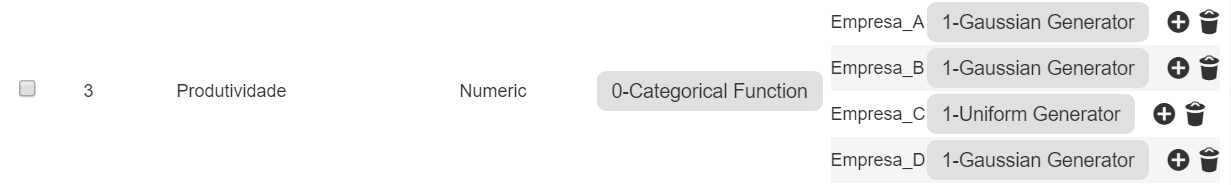
\includegraphics[width=\textwidth]{figures/geradorBlocks.png}
	\end{center}
	\legend{Fonte: O autor}
\end{figure}

\subsection{Perguntas a serem respondidas}
\begin{enumerate}
    \item Qual empresa apresenta os melhores indicadores em relação ao Faturamento de Lucratividade?
    

    \item Qual empresa tem pior taxa de satisfação dos colaboradores, e qual tem a melhor?
    

    \item Qual empresa tem os melhores indicadores de produtividade e quais são é sua concorrente mais próxima?

    
    \item Em relação a ''capacidade produtiva'' quais são as qual é a ordem das empresas do melhor para o pior?
    

    \item Qual empresa tem os piores indicadores em relação a retenção de talentos e capital intelectual “Turnover” e qual os melhores?
    
    
    
    
\end{enumerate}



\section{Visualização da Base}
Nesta seção será abordado as visualizações da base de dados sintética gerada foram elaborados alguns \textit{dashboard} com objetivo de extrair informações e visualizar os indicadores das empresas fictícias da base de dados e demonstrar a flexibilidade do protótipo.

\subsection{Propostas de \textit{Dashboards}}
\begin{itemize}
    \item \textbf{Proposta de Dashboard 1}:
    Na \autoref{vis_dashboard_empresas} é ilustrado a primeira proposta de \textit{dashboard}, a proposta elaborada tem como objetivo proporcionar a visualização de todos os KPIs presentes na base de dados para exploração e entendimento. A proposta é composta por 4 divisões as visualizações selecionas foram as seguintes matriz de \textit{scatterplot} para os KPIs do Financeiro,\textit{barchart} para os KPIs Clientes, coordenadas paralelas para os KPIs de Processos Internos, \textit{beeswarmplot} para os KPIs  de Aprendizado e Crescimento, esses respectivos KPIs estão descritos na \autoref{tabela_indicadores}
    
    \begin{figure}[h]
	    \caption{\label{vis_dashboard_empresas}
	    \textbf{Proposta de \textit{dashboard} 1}: \textit{dashboard} gerado com a base de dados sintética criada.
        }
	\begin{center}
	    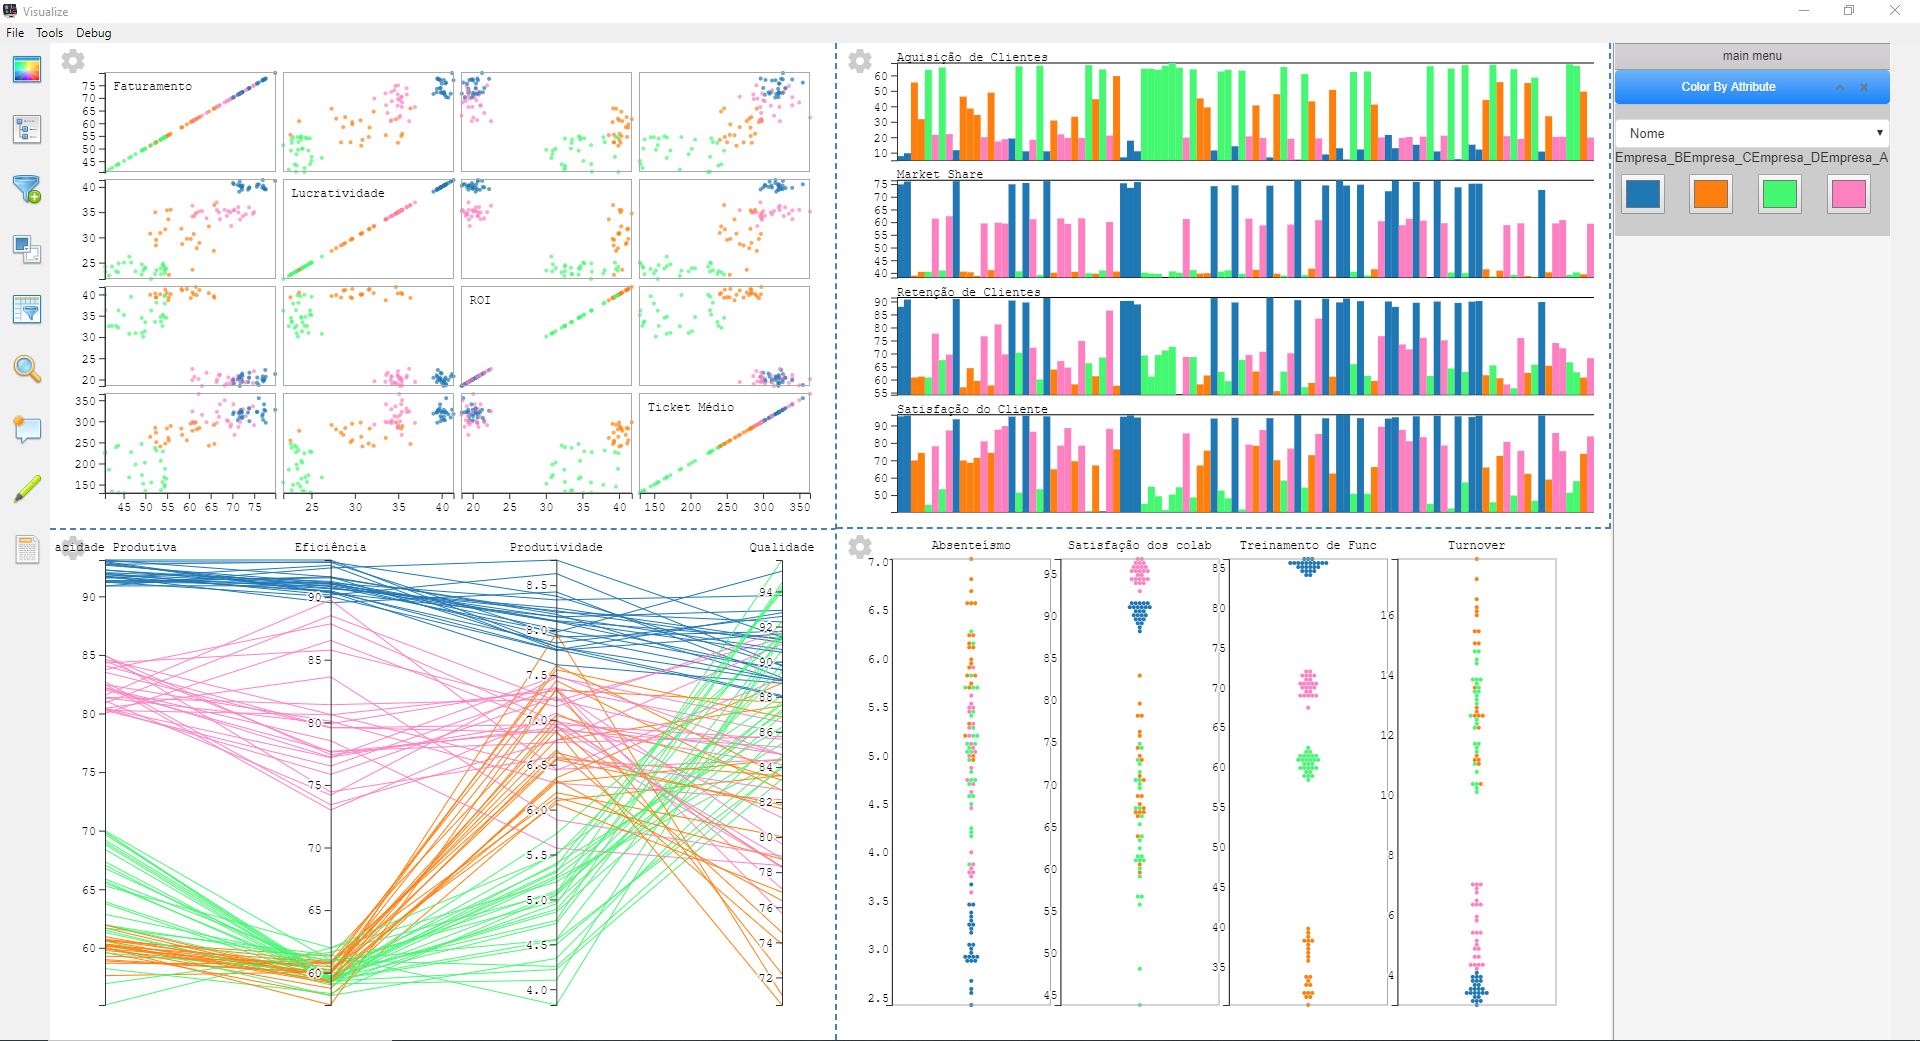
\includegraphics[width=\textwidth]{figures/dash1.png}
	\end{center}
	\legend{Fonte: O autor}
    \end{figure}

    \item \textbf{Proposta de  \textit{Dashboard} 2}:
     Na \autoref{fig_dash2} pode ser verificado a segunda proposta de \textit{dashboard} gerado na ferramenta, a proposta elaborada contém duas visualizações, diferente da proposta anterior essa propõe visualizações com menos dimensões para focar em atributos específicos, fornecendo uma proposta simplificada de \textit{dashboard}, os gráficos em tela tem mesmas cores nos itens, selecionados pelo atributo ''nome'', a primeira visualização é um \textit{treemap} com hierarquias pelo atributo ''nome'' e os tamanhos organizados pela ''produtividade''. A segunda visualização é uma matriz \textit{scatterplot} relacionado as colunas da base de dados sintética ''eficiência'' e ''lucratividade''.
    
    \begin{figure}[h]
	    \caption{\label{fig_dash2} \textbf{Proposta de \textit{dashboard} 2}: \textit{dashboard} gerado com a base de dados sintética criada.
        }
	\begin{center}
	    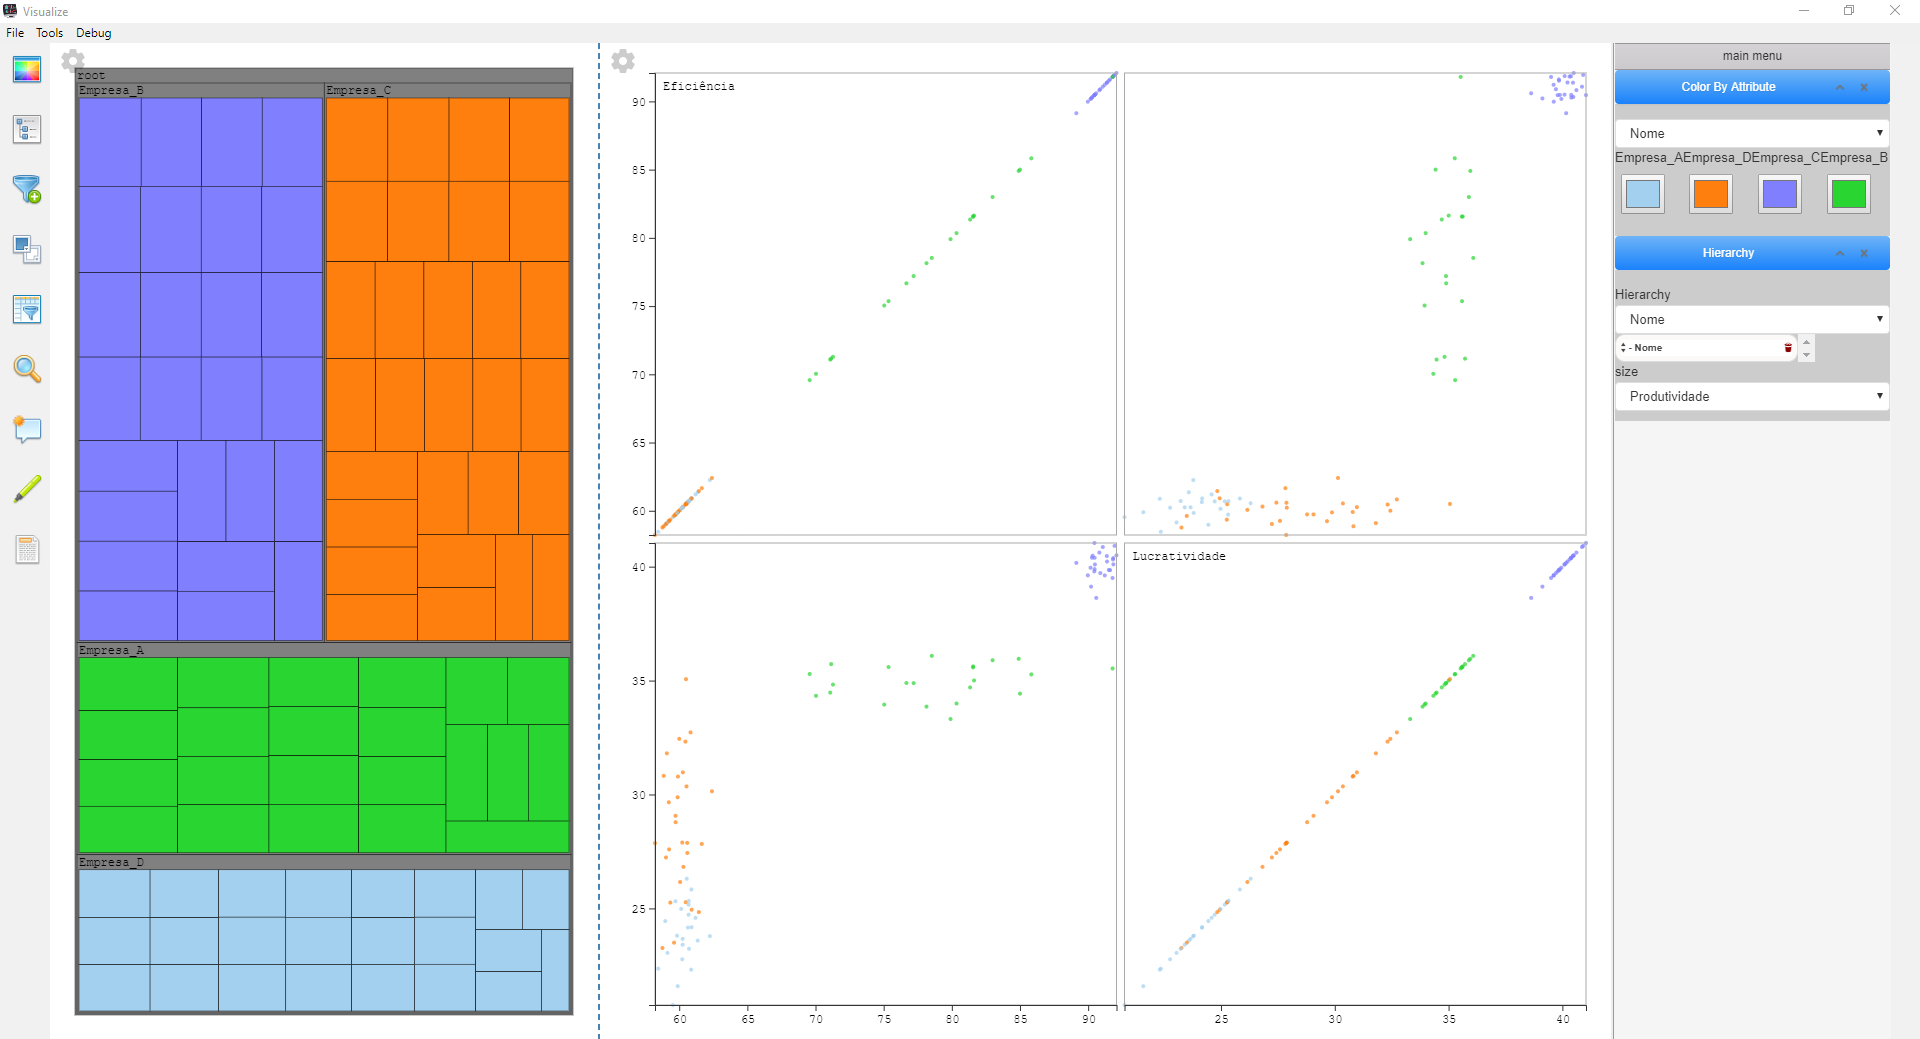
\includegraphics[width=\textwidth]{figures/dash2.png}
	\end{center}
	\legend{Fonte: O autor}
    \end{figure}

    \item \textbf{Proposta de \textit{Dashboard} 3}: Na \autoref{fig_dash3} é apresentado a terceira proposta de \textit{dashboard} gerada na ferramenta, essa proposta contém 4 visualizações com seus itens atribuídos com a mesma cor pelo atributo ''nome''. A primeira um gráfico de coordenadas paralelas contendo todas as dimensões da base de dados, isso para dar um visão geral dos dados, a segunda um \textit{sunburst} com hierarquias no nome e o tamanho dos item configurado para o atributo ''treinamento de funcionários'', um gráfico de barras indicando a coluna ''qualidade'' da base de dado, e por último um \textit{beeswarm plot} com na coluna de ''capacidade produtiva''. Essa proposta de \textit{dashboard} tem uma visão geral da base de dados, e em alguns pontos o foco em dimensões específicas como no \textit{beeswarm plot} e no gráfico de barras.
    
      \begin{figure}[h]
	    \caption{\label{fig_dash3} \textbf{Proposta de \textit{dashboard} 3}:\textit{dashboard} gerado com a base de dados sintética criada.
        }
	\begin{center}
	    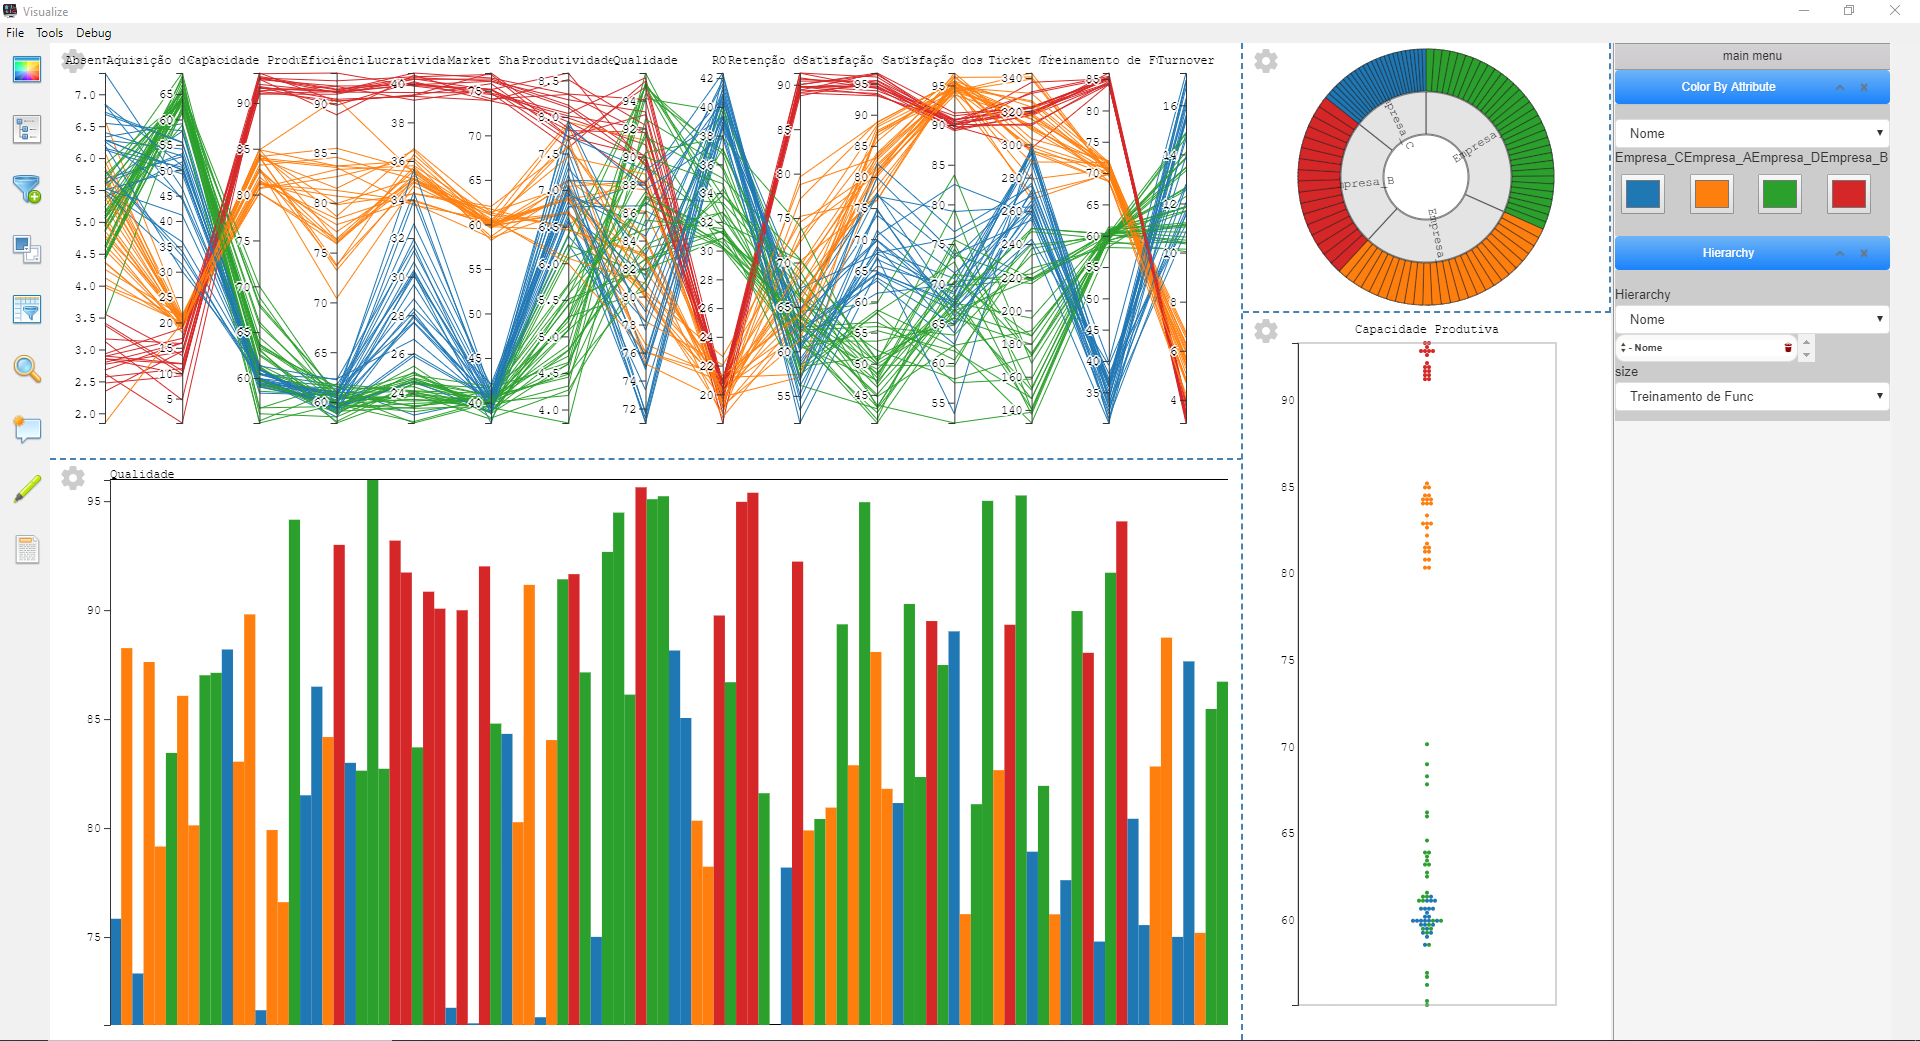
\includegraphics[width=\textwidth]{figures/dash3.png}
	\end{center}
	\legend{Fonte: O autor}
    \end{figure}


\end{itemize}

\chapter{Discussão e Resultados}
\label{ch:resultados}
Esta seção aborda os resultados e respostas do experimento de casos de uso e ao final uma discussão mais detalhada sobre a proposta de \textit{dashboard} e respostas obtidas sera desenvolvida nessa seção.

\section{Respostas Obtidas}
Das propostas de \textit{dashboards} para realização das avaliações e investigação das respostas, foi selecionado a proposta de \textit{dashboard} 1 pois suas quatro visualizações permitem a visualização de todas as dimensões da base de dados permitindo obter a resolução das perguntas levantadas.
As respostas das questões propostas sobre a base de dados podem ser visualizadas com mais detalhes na figura \autoref{fig_respostas} onde é destacado em cada resposta bem como resumo dos critérios de classificação desses indicadores podem ser observados na \autoref{resumo_Indicadores}.

\subsection{Questão 1}
 Na primeira pergunta em relação a quais empresas tem os melhores indicadores nas dimensões de ''faturamento'' e ''lucratividade'', observando a \autoref{fig_respostas} na matriz de \textit{scatterplot} em destaque temos dois círculos onde os itens de ''faturamento'' do maior para o menor seguem respectivamente a ''Empresa B'' e a ''Empresa A''. Na dimensão de ''lucratividade'' temos respectivamente a ''Empresa B'' e ''Empresa A'' levemente melhores, sendo essas duas que possuem os melhores indicadores nessa dimensão.

\subsection{Questão 2}
Na segunda questão é ilustrado a resposta \autoref{fig_respostas} observando o \textit{beeswarm plot} no item 2 pode ser percebido que a ''Empresa C'' tem os piores dados de indicadores em relação a ''satisfação dos colaboradores'' e a ''Empresa A'' tem os melhores indicadores para esse KPI, destacados nos círculos na \autoref{fig_respostas}.

\subsection{Questão 3} 
Na terceira questão a localização da resposta, pode ser obtida visualizando a \autoref{fig_respostas}. No gráfico coordenadas paralelas no item 3 a dimensão ''produtividade'' nessa dimensão dos itens mais alto para os mais baixos, temos respectivamente no primeiro lugar a ''Empresa B'' em segundo lugar a ''Empresa C'' mesmo essa empresa tendo uma dispersão maior dos dados que a ''Empresa A'' os maiores indicadores para segundo lugar pertencem a ''Empresa C''.

\subsection{Questão 4}
A quarta questão observando o item 4 no gráfico de paralelas coordenas respectivamente na dimensão de ''capacidade produtiva'' do maior para o menor ilustrado na \autoref{resumo_Indicadores} as empresas em relação a capacidade produtiva seguem a ordem da melhor para o pior empresa no caso respectivamente a ''Empresa B'', ''Empresa A'', ''Empresa C'' , e ''Empresa D''. Analisando a ''Empresa C'' temos uma dispersão média do dados menor que a ''Empresa D'' porém a ''Empresa D'' contém melhores dados com menores itens em relação nessa dimensão a colocando como última da lista. 

\subsection{Questão 5}
Na quinta questão o item 5 no gráfico \textit{beeswarm plot}, na \autoref{fig_respostas}, pode ser localizada desde a pior até a melhor empresa em relação ao  índice de ''Turnover''. O pior desempenho nesse indicador encontra-se na ''Empresa C'' entre 5\% e 10\% indicado como pior em situação de ''Alerta'', e a ''Empresa B'' tem a melhor classificação menor que 5\% definido como ''OK''.

\section{Avaliações}

A proposta de \textit{dashboard} 1 foi elaborada e seleciona para resolução dessas questões, a pois a separação das 4 visualizações permite um \textit{overview} completo da base de dados, utilizando o gráfico de coordenadas paralelas é possível visualizar todas as colunas da base de dados com ilustrado na \autoref{fig_dash3} na proposta de \textit{dashboard} 3, porém uma divisão e dos tipos de KPI's podem facilitar a localização e análise das informações. Bem como, a possibilidade de ter uma visão focalizado em apenas uma dimensão ilustrado na \autoref{fig_dash3} em diferentes casos em que as demais colunas não seriam necessárias permitiria melhora aproveitamento do espaço em tela para criação para criação de outras visualizações.

A proposta de \textit{dashboard} 2 não possibilita a resolução de todas as questões propostas, porém uma visualização reduzida com apenas algumas colunas pode ser um caso de uso necessários em diferentes situações de uma empresa de uma maneira mais eficiente. O gráfico de \textit{treemap} permite a separação por meio das hierarquias dividindo as 4 empresas de observando as dimensões, porém caso os itens tenham uma proximidade é possível que ocasione dúvidas com esse gráfico, além disso com alguns tratamentos na base de dados é possível criar outra sub hierarquias com base na tabela na \autoref{resumo_Indicadores}

Desse modo explorando as outras propostas de \textit{dashboards} podem responder algumas das questões levantas com eficiência porém conforme analise das questões o mais indicado para conseguir responder com eficiência e eficácia nesse trabalho é o \textit{ dashboard} 1.

   \begin{figure}[h]
	    \caption{\label{fig_respostas} \textit{Dashboard} proposto com as respostas das questões, em destaque temos o item 1 a primeira resposta e seus dois itens em destaque a melhor e pior empresa, o item 2 a melhor e pior empresa na dimensão, o item 3 as duas primeiras na dimensão, o item 4 a ordem das empresas na dimensão, o item 5 a resposta do melhor e pior na dimensão.
        }
	\begin{center}
	    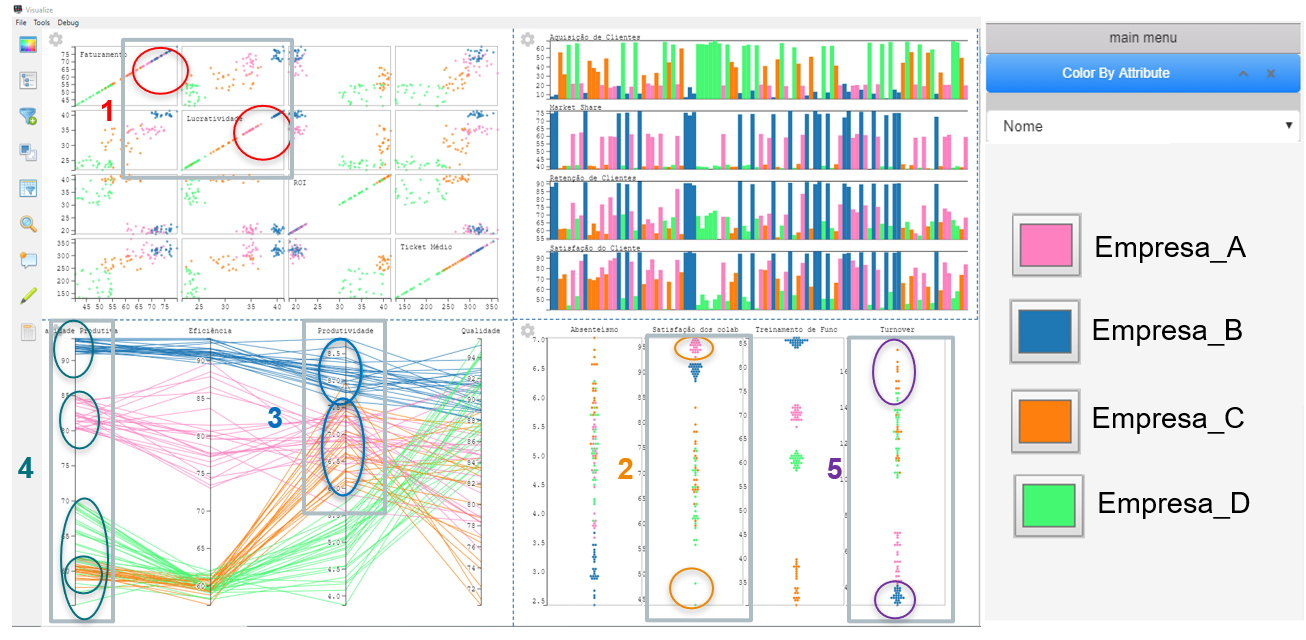
\includegraphics[width=\textwidth,height=22pc]{figures/respostas.png}
	\end{center}
	\legend{Fonte: O autor}
    \end{figure}



\chapter{Considerações Finais e Trabalhos Futuros}
\label{ch:conclusao}

Nesse trabalho de conclusão de curso foi desenvolvido uma ferramenta capaz de criar \textit{dashboards} de forma interativa e incremental, desde a definição do layout das divisões até a seleção de quais visualizações estarão nas respectivas divisões. A aplicação pode gerar um conjunto de técnicas de \textit{Infovis} e fornece interações para trabalhar essas técnicas de maneira coordenada.  

A criação de \textit{layouts} de tela e definição de visualizações presentes em cada divisão por meio de um arquivo JSON, com a exportação e importação permite a comunicação com outras ferramentas. Desse modo, sendo possível em trabalhos futuros em conjunto com trabalho de aprendizagem de máquina definir qual layout seria ideal para cada base de dados, e esses layouts já serem importados pela aplicação automaticamente para o usuário. Bem como, seria possível definir ainda por meio de aprendizado de máquina quais as melhores visualizações dependendo da base de dados.

As visualizações selecionadas, carregam diferentes características com possibilidades diversas para criação de diferentes \textit{dashboards} com customizações e interações, bem como a possibilidade de exportar tanto os layouts quanto as visualizações \textit{dashboards} para uso posterior pela ferramenta.

Como uma proposta de trabalho futuro pretendemos criar uma funcionalidade envolvendo aprendizado de máquina onde seja possível o próprio sistema sugerir layout de \textit{dashboard} dependendo da base de dados, com um passo de validação pelo usuário de como ficarão exibidas em tela as visualizações disponíveis. Além disso, a implementação de outras visualizações pode ser realizadas para utilização em outros contextos como \textit{piechart}, \textit{wordcloud}, \textit{heatmap} e \textit{linechart}.

Outro trabalho futuro é a migração dessa aplicação \textit{desktop} para uma aplicação SPA disponível em um servidor online, ficando assim disponível em servidor com domínio para acesso dos usuários e também realizar integração com banco de dados SQL. Estando em um ambiente online a aplicação terá um novo leque de possibilidades como um módulo multiusuário, permitindo vários usuários acessarem um ambiente colaborativo online e reativo para modelagem de um \textit{dashboard} ou exploração e análise do mesmo. Para realização dessas propostas além da migração para deixar a aplicação online será necessário um módulo de gerenciamento e permissões de usuários em tempo real no ambiente online.

Finalizando é necessário avaliar a aplicação com usuários experientes e inexperientes, propondo tarefas de visualização de dados para avaliar a usabilidade da ferramenta e identificar novas necessidades em relação aos \textit{dashboards}, da mesma forma avaliar os pontos positivos e negativos.






% % ----------------------------------------------------------
% % Introdução (exemplo de capítulo sem numeração, mas presente no Sumário)
% % ----------------------------------------------------------
% \chapter{Introdução}
% % ----------------------------------------------------------



% \lipsum[31-33]

% ----------------------------------------------------------
% ELEMENTOS PÓS-TEXTUAIS
% ----------------------------------------------------------
\postextual
% ----------------------------------------------------------

% ----------------------------------------------------------
% Referências bibliográficas
% ----------------------------------------------------------
\bibliography{abntex2-modelo-references}

% ----------------------------------------------------------
% Glossário
% ----------------------------------------------------------
%
% Consulte o manual da classe abntex2 para orientações sobre o glossário.
%
%\glossary

% ----------------------------------------------------------
% Apêndices
% ----------------------------------------------------------

% ---
% Inicia os apêndices
% ---
% \begin{apendicesenv}

% Imprime uma página indicando o início dos apêndices
% \partapendices

% ----------------------------------------------------------
% \chapter{Quisque libero justo}
% ----------------------------------------------------------

% \lipsum[50]

% ----------------------------------------------------------
% \chapter{Nullam elementum urna vel imperdiet sodales elit ipsum pharetra ligula
% ac pretium ante justo a nulla curabitur tristique arcu eu metus}
% ----------------------------------------------------------
% \lipsum[55-57]

% \end{apendicesenv}
% ---


% ----------------------------------------------------------
% Anexos
% ----------------------------------------------------------

% ---
% Inicia os anexos
% ---
\begin{anexosenv}

% Imprime uma página indicando o início dos anexos
\partanexos

\chapter{Arquivo para realizar a geração da base de dados sintética na ferramenta Blocks\cite{blocks}. }
\label{ch:anexo}

\begin{minted}{json}
{
 "name": "empresas", "generator":[{
   "name": "Nome",
   "type": "Categorical","ID": "COL_8wf5geo35.sa","display": true,
   "generator": [{
     "name": "Categorical","order": 0,"ID":"GEN_fftdlaqg.9vc",
     "accessOperator": "sum",
     "array": ["Empresa_A","Empresa_B","Empresa_C","Empresa_D"
    ]}]}
  {
   "name": "Tempo","type": "Time","ID": "COL_2j5gu9uqd.65",
   "display": true,   "generator": [{
     "name": "Fixed Time Generator","order": 0,"ID": "GEN_c92ie91a.dys",
     "accessOperator": "sum",
     "begin": 0,"step": 1,"initTime": "08:00:00","strStep": "01:00:10",
     "timeMask": "HH:mm:ss"}]},
  {
   "name": "Produtividade","type": "Numeric","ID": "COL_3o5602aw.ira",
   "display": true,   "generator": [{
     "name": "CategoricalFunction","order": 0,"ID": "GEN_6w81na6y0.vs",
     "accessOperator": "none","inputGenIndex": 0,
     "listOfGenerators": {
      "Empresa_A": [{
        "name": "Gaussian Generator","order": 1,"ID":"GEN_2zgaweootl.2",
        "accessOperator": "sum",
        "mean": 7,"std": 0.5
       }],
      "Empresa_B": [{
        "name": "GaussianGenerator","order": 1,"ID": "GEN_1votnehwz.ct",
        "accessOperator": "sum","mean": 8,"std": 0.3
       }],
      "Empresa_C":[{
        "name": "Uniform Generator","order": 1,"ID": "GEN_9er8ugha.k5j",
        "accessOperator": "sum",
        "min": 6,"max": 8,"disc": false
       }],
      "Empresa_D":[{
        "name": "Gaussian Generator","order": 1,"ID": "GEN_hdw6ksy4.dja",
        "accessOperator": "sum",
        "mean": 5,"std": 0.6
       }]}},
    {
     "name": "Uniform Generator","order": 0,"ID": "GEN_4dytf260.xyx",
     "accessOperator": "sum",
     "min": 0,"max": 1,"disc": false
     "min": 0,"max": 1,"disc": false}]},
  {
   "name": "Lucratividade","type": "Numeric","ID": "COL_1rnhjl69u.yp",
   "display": true,   "generator": [{
     "name": "Categorical Function","order": 0,"ID": "GEN_mjpgzlzs.9oo",
     "accessOperator": "none",
     "inputGenIndex": 0,
     "listOfGenerators": {
      "Empresa_A": [{
        "name": "Gaussian Generator","order": 1,"ID": "GEN_fjx81zuz.zno",
        "accessOperator": "sum","mean": 35,"std": 0.9
       }],
      "Empresa_B": [{
        "name": "Gaussian Generator","order": 1,"ID": "GEN_1ymc7o7h55.q",
        "accessOperator": "sum","mean": 40,"std": 0.5
       }],
      "Empresa_C": [{
        "name": "Gaussian Generator","order": 1,"ID": "GEN_1ogw7cbni.7u",
        "accessOperator": "sum","mean": 30,"std": 3
       }],
      "Empresa_D": [{
        "name": "Gaussian Generator","order": 1,"ID": "GEN_1fnywz5av.yqg",
        "accessOperator": "sum","mean": 24,"std": 1
       }]}},{
     "name": "Uniform Generator","order": 0,"ID": "GEN_38wv08wgi.e",
     "accessOperator": "sum",
     "min": 0,"max": 1,"disc": false}]},
{
   "name": "Capacidade Produtiva",
   "type": "Numeric",
   "ID": "COL_24rl910y4.lf",
   "display": true,
   "generator": [{
     "name": "Categorical Function","order": 0,"ID": "GEN_j45v3bj6.kke",
     "accessOperator": "sum","inputGenIndex": 0,
     "listOfGenerators": {
      "Empresa_A": [{
        "name": "Uniform Generator","order": 0,"ID": "GEN_3q724b1.t1bf",
        "accessOperator": "sum",
        "min": 80,"max": 85,"disc": false
       }],
      "Empresa_B": [{
        "name": "Gaussian Generator","order": 0,"ID": "GEN_ml8l1t56.4h",
        "accessOperator": "sum","mean": 92,"std": 0.6
       }],
      "Empresa_C": [{
        "name": "Gaussian Generator","order": 0,"ID": "GEN_m1717hht.lfq",
        "accessOperator": "sum","mean": 60,"std": 0.8
       }],
      "Empresa_D": [{
        "name": "Uniform Generator","order": 0,"ID": "GEN_ojvwkzjt.xec",
        "accessOperator": "none","min": 55,"max": 70,
        "disc": false
      }]}},
    {
     "name": "Uniform Generator","order": 0,"ID": "GEN_8wl4xsxr.qs",
     "accessOperator": "sum","min": 0,"max": 1,"disc": false}]},
  {
   "name": "Qualidade",
   "type": "Numeric",
   "ID": "COL_1sjf53od2.zm",
   "display": true,
   "generator": [{
     "name": "Categorical Function","order": 0,"ID": "GEN_41i0qchj.cs",
     "accessOperator": "none","inputGenIndex": 0,
     "listOfGenerators": {
      "Empresa_A": [{
        "name": "Uniform Generator","order": 0,"ID": "GEN_9jm5ipeq.jcw",
        "accessOperator": "sum","min": 75,"max": 92,
        "disc": false
       }],
      "Empresa_B": [{
        "name": "Uniform Generator","order": 0,"ID": "GEN_9rkynjkr.cur",
        "accessOperator": "sum","min": 88,"max": 96,"disc": false
       }],
      "Empresa_C": [{
        "name": "Uniform Generator","order": 0,"ID": "GEN_21ozt6lcb.ow",
        "accessOperator": "sum","min": 70,"max": 90,
        "disc": false
       }],
      "Empresa_D": [{
        "name": "Uniform Generator","order": 0,"ID": "GEN_2a7mkr2v7.6r",
        "accessOperator": "sum","min": 80,"max": 96,
        "disc": false
      }]}},
    {
     "name": "Uniform Generator","order": 0,"ID": "GEN_dosysqex.0zr",
     "accessOperator": "sum",
     "min": 0,"max": 1,"disc": false}]},
  {
   "name": "Eficiência","type": "Numeric","ID": "COL_9gmi6dfn.32",
   "display": true,   "generator": [{
     "name": "Categorical Function","order": 0,"ID": "GEN_oie9sfy1.316",
     "accessOperator": "none","inputGenIndex": 0,
     "listOfGenerators": {
      "Empresa_A": [{
        "name": "Gaussian Generator","order": 0,"ID": "GEN_t5nvn76h.cf",
        "accessOperator": "sum","mean": 80,"std": 5
       }],
      "Empresa_B": [{
        "name": "Gaussian Generator","order": 0,"ID": "GEN_wqs875in.t",
        "accessOperator": "sum","mean": 91,"std": 0.8
       }],
      "Empresa_C": [{
        "name": "Gaussian Generator","order": 0,"ID": "GEN_13qwzdsu4.va",
        "accessOperator": "sum","mean": 60,"std": 1
       }],
      "Empresa_D": [{
        "name": "Gaussian Generator","order": 0,"ID": "GEN_v8njd213.nl",
        "accessOperator": "sum","mean": 60,"std": 1
     }]}},
    {
     "name": "Uniform Generator","order": 0,"ID": "GEN_a14jg52p.kda",
     "accessOperator": "sum",
     "min": 0,"max": 1,"disc": false}]},
  {
   "name": "Satisfação do Cliente",
   "type": "Numeric",
   "ID": "COL_zm8rjon9.sb",
   "display": true,   "generator": [{
     "name": "Categorical Function","order": 0,"ID": "GEN_wrvewm3k.gqg",
     "accessOperator": "none","inputGenIndex": 0,
     "listOfGenerators": {
      "Empresa_A": [{
        "name": "Uniform Generator","order": 0,"ID": "GEN_1mss5p7d.kkzf",
        "accessOperator": "sum","min": 75,"max": 90,"disc": false
       }],
      "Empresa_B": [{
        "name": "Gaussian Generator","order": 0,"ID": "GEN_6bfphuad7.yw",
        "accessOperator": "sum","mean": 95,"std": 1
       }],
      "Empresa_C": [{
        "name": "Gaussian Generator","order": 0,"ID": "GEN_ly243vaw.zk6",
        "accessOperator": "sum","mean": 70,"std": 5
       }],
      "Empresa_D": [{
        "name": "Uniform Generator","order": 0,"ID": "GEN_jdslm5xz.yre",
        "accessOperator": "sum",
        "min": 60,"max": 40,"disc": false
     }]}},
    {
     "name": "Uniform Generator","order": 0,"ID": "GEN_fqwjeiif.y2p",
     "accessOperator": "sum","min": 0,"max": 1,"disc": false}]},
  {
   "name": "Retenção de Clientes",
   "type": "Numeric",
   "ID": "COL_27hi19bie.mw",
   "display": true,   "generator": [{
     "name": "Categorical Function","order": 0,"ID": "GEN_me1ygb06.d9",
     "accessOperator": "none","inputGenIndex": 0,
     "listOfGenerators": {
      "Empresa_A": [{
        "name": "Gaussian Generator","order": 0,"ID": "GEN_acrkceq2.bja",
        "accessOperator": "sum","mean": 70,"std": 6
       }],
      "Empresa_B": [{
        "name": "Gaussian Generator","order": 0,"ID": "GEN_29v66xta.v11",
        "accessOperator": "sum","mean": 90,"std": 1
       }],
      "Empresa_C": [{
        "name": "Gaussian Generator","order": 0,"ID": "GEN_1ctthqzhb.3kh",
        "accessOperator": "sum","mean": 60,"std": 3
       }],
      "Empresa_D": [{
        "name": "Gaussian Generator","order": 0,"ID":"GEN_1dzfqw8qk.goj",
        "accessOperator": "sum","mean": 65,"std": 5
     }]}},
    {
     "name": "Uniform Generator","order": 0,"ID": "GEN_1061a1j2t.c8g",
     "accessOperator": "sum","min": 0,"max": 1,"disc": false}]},
  {
   "name": "Custo de Aquisição",
   "type": "Numeric",
   "ID": "COL_2wj5lmur.20c",
   "display": true,"generator": [{
     "name": "Categorical Function","order": 0,"ID": "GEN_g1e728mc.3zc",
     "accessOperator": "none","inputGenIndex": 0,
     "listOfGenerators": {
      "Empresa_A": [{
        "name": "Gaussian Generator","order": 0,"ID": "GEN_604jyw8m.w07",
        "accessOperator": "sum","mean": 20,"std": 1
       }],
      "Empresa_B": [{
        "name": "Gaussian Generator","order": 0,"ID": "GEN_8h5ffg15.tm",
        "accessOperator": "sum","mean": 10,"std": 5
       }],
      "Empresa_C": [{
        "name": "Uniform Generator","order": 0,"ID": "GEN_akoblpix.nlv",
        "accessOperator": "sum","min": 30,"max": 60,"disc": false
       }],
      "Empresa_D": [{
        "name": "Gaussian Generator","order": 0,"ID": "GEN_7sgppu4x.nt5",
        "accessOperator": "sum","mean": 65,"std": 2
     }]}},
    {
     "name": "Uniform Generator","order": 0,"ID": "GEN_69i9snrd.ya2",
     "accessOperator": "sum","min": 0,"max": 1,"disc": false}]},
  {
   "name": "Market Share","type": "Numeric","ID": "COL_217ieo4w.gma",
   "display": true,   "generator": [{
     "name": "Categorical Function","order": 0,"ID": "GEN_1e0jfdwrb.0p",
     "accessOperator": "none",
     "inputGenIndex": 0,
     "listOfGenerators": {
      "Empresa_A": [{
        "name": "Gaussian Generator","order": 0,"ID": "GEN_560b059ln.k1",
        "accessOperator": "sum","mean": 60,"std": 1
       }],
      "Empresa_B": [{
        "name": "Gaussian Generator","order": 0,"ID": "GEN_d8y359lt.24f",
        "accessOperator": "sum","mean": 75,"std": 1
       }],
      "Empresa_C": [{
        "name": "Gaussian Generator","order": 0,"ID": "GEN_200npht46.44",
        "accessOperator": "sum","mean": 40,"std": 1
       },
       {
        "name": "Get Extra Value","order": 1,"ID": "GEN_lu07qyod.m9sc",
        "accessOperator": "sum","extra_index": 1,
        "srcGen": ""
       }],
      "Empresa_D": [{
        "name": "Gaussian Generator","order": 0,"ID": "GEN_c2uk0jivz.7w",
        "accessOperator": "sum","mean": 40,"std": 1
     }]}},
    {
     "name": "Uniform Generator","order": 0,"ID": "GEN_l16bj400.jtt",
     "accessOperator": "sum","min": 0,"max": 1,"disc": false}]},
  {
   "name": "Turnover","type": "Numeric",
   "ID": "COL_pka70f43.tp","display": true,
   "generator": [{
     "name": "Categorical Function","order": 0,"ID": "GEN_f7d62r4hy.z6",
     "accessOperator": "none","inputGenIndex": 0,
     "listOfGenerators": {
      "Empresa_A": [{
        "name": "Uniform Generator","order": 0,"ID": "GEN_f2lrt2x5.ey",
        "accessOperator": "sum","min": 4,"max": 7,"disc": false
       }],
      "Empresa_B": [{
        "name": "Uniform Generator","order": 0,"ID": "GEN_30etsymo0.bm",
        "accessOperator": "sum","min": 3,"max": 4,"disc": false
       }],
      "Empresa_C": [{
        "name": "Uniform Generator","order": 0,"ID": "GEN_1uhl8tmqe.rj",
        "accessOperator": "sum","min": 10,"max": 18,"disc": false
       }],
      "Empresa_D": [{
        "name": "Uniform Generator","order": 0,"ID": "GEN_1ulic8sq3.tc",
        "accessOperator": "sum","min": 10,"max": 15,"disc": false
     }]}},
    {
     "name": "Uniform Generator","order": 0,"ID": "GEN_7omxqh3w.x78",
     "accessOperator": "sum","min": 0,"max": 1,"disc": false}]},
  {
   "name": "Treinamento de Func",
   "type": "Numeric","ID": "COL_9yswoimx.yp","display": true,
   "generator": [{
     "name": "Categorical Function","order": 0,"ID": "GEN_1427nenau.5y",
     "accessOperator": "none",
     "inputGenIndex": 0,"listOfGenerators": {
      "Empresa_A": [{
        "name": "Gaussian Generator","order": 0,"ID": "GEN_sthpx2d8.2k",
        "accessOperator": "sum","mean": 70,"std": 1
       }],
      "Empresa_B": [{
        "name": "Gaussian Generator","order": 0,"ID": "GEN_deoqsaj0.nrw",
        "accessOperator": "sum","mean": 85,"std": 0.7
       }],
      "Empresa_C": [{
        "name": "Uniform Generator","order": 0,"ID": "GEN_19oyw2cr3.aif",
        "accessOperator": "sum","min": 30,"max": 40,"disc": false
       }],
      "Empresa_D": [{
        "name": "Gaussian Generator","order": 0,"ID": "GEN_2ti8mplwp.p9",
        "accessOperator": "sum","mean": 60,"std": 1
     }]}},
    {
     "name": "Uniform Generator","order": 0,"ID": "GEN_23clohum.thi",
     "accessOperator": "sum","min": 0,"max": 1,"disc": false}]},
  {
   "name": "Satisfação dos colab","type": "Numeric",
   "ID": "COL_1mz4mzrq7.bn","display": true,
   "generator": [{
     "name": "Categorical Function","order": 0,"ID": "GEN_122n192xf.lv",
     "accessOperator": "none","inputGenIndex": 0,
     "listOfGenerators": {
      "Empresa_A": [{
        "name": "Gaussian Generator","order": 0,"ID": "GEN_2d953g0dk.a1",
        "accessOperator": "sum","mean": 95,"std": 1
       }],
      "Empresa_B": [{
        "name": "Gaussian Generator","order": 0,"ID": "GEN_lqhx9ydw.lyp",
        "accessOperator": "sum","mean": 90,"std": 1
       }],
      "Empresa_C": [{
        "name": "Gaussian Generator","order": 0,"ID": "GEN_cj3l3exa.a63",
        "accessOperator": "sum","mean": 70,"std": 7
       }],
      "Empresa_D": [{
        "name": "Gaussian Generator","order": 0,"ID": "GEN_6i5p9r0p.kf9",
        "accessOperator": "sum","mean": 65,"std": 8
}]}},
    {
     "name": "Uniform Generator","order": 0,"ID": "GEN_6ku24aka.lz",
     "accessOperator": "sum","min": 0,"max": 1,"disc": false}]},
  {"name": "Absenteísmo","type": "Numeric",
   "ID": "COL_t6tazorv.q2",
   "display": true,
   "generator": [{
     "name": "Categorical Function","order": 0,"ID": "GEN_oz5hhme2.i2j",
     "accessOperator": "none","inputGenIndex": 0,
     "listOfGenerators": {
      "Empresa_A": [{
        "name": "Gaussian Generator","order": 0,"ID": "GEN_apj0fovi.tzf",
        "accessOperator": "sum","mean": 5,"std": 0.8
       }],
      "Empresa_B": [{
        "name": "Gaussian Generator","order": 0,"ID": "GEN_3gc7d8nc.agj",
        "accessOperator": "sum","mean": 3,"std": 0.3
       }],
      "Empresa_C": [{
        "name": "Gaussian Generator","order": 0,"ID": "GEN_ogtqckyp.537",
        "accessOperator": "sum","mean": 6,"std": 0.5
       }],
      "Empresa_D": [{
        "name": "Gaussian Generator","order": 0,"ID": "GEN_1g2j0d4sl.nq",
        "accessOperator": "sum","mean": 5,"std": 0.5
}]}},
    {
     "name": "Uniform Generator","order": 0,"ID": "GEN_m6o0ujqe.c08",
     "accessOperator": "sum","min": 0,"max": 1,"disc": false}]},
  {
   "name": "ROI","type": "Numeric",
   "ID": "COL_q1jtxw7d.euq",
   "display": true,
   "generator": [{
     "name": "Categorical Function","order": 0,"ID": "GEN_i3rpyezy.v5o",
     "accessOperator": "none",
     "inputGenIndex": 0,
     "listOfGenerators": {
      "Empresa_A": [{
        "name": "Gaussian Generator","order": 0,"ID": "GEN_wtauagpc.82h",
        "accessOperator": "sum","mean": 20,"std": 1
       }],
      "Empresa_B": [{
        "name": "Gaussian Generator","order": 0,"ID": "GEN_7wjh23y7.kke",
        "accessOperator": "sum","mean": 20,"std": 1
       }],
      "Empresa_C": [{
        "name": "Gaussian Generator","order": 0,"ID": "GEN_v306zkbt.ymn",
        "accessOperator": "sum","mean": 40,"std": 1
       }],
      "Empresa_D": [{
        "name": "Uniform Generator","order": 0,"ID": "GEN_197r6al6q.1v",
        "accessOperator": "sum","min": 30,"max": 40,"disc": false
}]}},
    {
     "name": "Uniform Generator",
     "order": 0,"ID": "GEN_6wc6gkwy.hz8",
     "accessOperator": "sum",
     "min": 0,"max": 1,"disc": false}]},
  {
   "name": "Faturamento","type": "Numeric",
   "ID": "COL_bgq8csq2y.q6","display": true,
   "generator": [{
     "name": "Categorical Function","order": 0,"ID": "GEN_c3vc7br.k2hm",
     "accessOperator": "none","inputGenIndex": 0,
     "listOfGenerators": {
      "Empresa_A": [{
        "name": "Gaussian Generator","order": 0,"ID": "GEN_s1gmkok.b9d",
        "accessOperator": "sum","mean": 55,"std": 5
       }],
      "Empresa_B": [{
        "name": "Gaussian Generator","order": 0,"ID": "GEN_1tzn1nskz.ac",
        "accessOperator": "sum","mean": 77,"std": 10
       }],
      "Empresa_C": [{
        "name": "Gaussian Generator","order": 0,"ID": "GEN_5qhsjwh7.9or",
        "accessOperator": "sum","mean": 40,"std": 3
       }],
      "Empresa_D": [{
        "name": "Gaussian Generator","order": 0,"ID": "GEN_a0r6ej9t.rqr",
        "accessOperator": "sum","mean": 40,"std": 3
}]}},
    {
     "name": "Uniform Generator","order": 0,"ID": "GEN_14paev7yi.6m",
     "accessOperator": "sum","min": 0,"max": 1,"disc": false}]},
  {
   "name": "Tiket Médio","type":"Numeric","ID": "COL_bopp0tkg.aj8",
   "display": true,
   "generator":[{
     "name": "Categorical Function","order": 0,"ID": "GEN_551yftc7g.5k",
     "accessOperator": "none","inputGenIndex": 0,
     "listOfGenerators": {
      "Empresa_A": [{
        "name": "Uniform Generator","order": 0,"ID": "GEN_2rv1ddfjf.zb",
        "accessOperator": "sum","min": 220,"max": 280,
        "disc": false
       }],
      "Empresa_B":[{
        "name": "Uniform Generator","order": 0,"ID": "GEN_wx5bzl48.tt",
        "accessOperator": "sum","min": 310,"max": 330,
        "disc": false
       }],
      "Empresa_C": [{
        "name": "Gaussian Generator","order": 0,"ID": "GEN_hygr07tn.dh",
        "accessOperator": "sum","mean": 310,"std": 10
       }],
      "Empresa_D": [{
        "name": "Uniform Generator","order": 0,"ID": "GEN_ww77b46d.woe",
        "accessOperator": "sum","min": 140,"max":220,"disc": false
       }
    ]}},{
     "name": "Uniform Generator","order": 0,"ID": "GEN_5w84m7o1.u6y",
     "accessOperator": "sum",
     "min": 0,"max": 1,"disc": false
}]}],
 "n_lines": 100,"step_lines": 10000,"columnsCounter": 36,"save_as": "csv",
 "header": true,"header_type": true
}
\end{minted}

\end{anexosenv}
\end{document}
% https://pt.overleaf.com/project/60a453de92ea58387e2a7ad8